% !TEX encoding = UTF-8 Unicode
% ------------------------------------------------------------------------------
% Este fichero es parte de la plantilla LaTeX para la realización de Proyectos
% Final de Grado, protegido bajo los términos de la licencia GFDL.
% Para más información, la licencia completa viene incluida en el
% fichero fdl-1.3.tex

% Copyright (C) 2012 SPI-FM. Universidad de Cádiz
% ------------------------------------------------------------------------------


\documentclass[a4paper,11pt]{book}

% PAQUETES
\usepackage[spanish]{babel} % para escribir en español
\usepackage{./estilo/paquetes}
\usepackage{./estilo/colores}
\usepackage{./estilo/comandos}
\usepackage[utf8]{inputenc}
\usepackage{multirow, array} % para las tablas
\usepackage{float} % para usar [H]
\usepackage{tabularx} % para el ancho de tablas

% Ruta al directorio de imágenes
\graphicspath{{./img/}} 

% METADATOS
\title{MEMORIA DEL PFC: GESTIÓN DE CENTRO DE MEJORA DEL RENDIMIENTO Y LA SALUD}
\author{Jesús Soriano Candón}
\date{\today} 
 
\begin{document}

\pagestyle{plain}

% PORTADAS
% !TEX encoding = UTF-8 Unicode
% ------------------------------------------------------------------------------
% Este fichero es parte de la plantilla LaTeX para la realización de Proyectos
% Final de Grado, protegido bajo los términos de la licencia GFDL.
% Para más información, la licencia completa viene incluida en el
% fichero fdl-1.3.tex

% Copyright (C) 2012 SPI-FM. Universidad de Cádiz
% ------------------------------------------------------------------------------


\begin{titlepage}

  \begin{center}

    
\includegraphics[width=0.3\textwidth]{logo-uca.png} \\
    
    \vspace{2.5cm}
    
    \LARGE{\textbf{ESCUELA SUPERIOR DE INGENIERÍA}} \\
    
    \vspace{1.0cm}
    
    \Large{\textbf{INGENIERÍA INFORMÁTICA}} \\
    
    \vspace{3.0cm}
    
    \Large{GESTIÓN DE CENTRO DE MEJORA DEL RENDIMIENTO Y LA SALUD} \\
    
    \vspace{2.5cm}
    
    \Large{Jesús Soriano Candón} \\
  
    \vspace{0.5cm}

    \large{\today}
    
  \end{center}
\end{titlepage}

\cleardoublepage

% !TEX encoding = UTF-8 Unicode
% ------------------------------------------------------------------------------
% Este fichero es parte de la plantilla LaTeX para la realización de Proyectos
% Final de Grado, protegido bajo los términos de la licencia GFDL.
% Para más información, la licencia completa viene incluida en el
% fichero fdl-1.3.tex

% Copyright (C) 2012 SPI-FM. Universidad de Cádiz
% ------------------------------------------------------------------------------


\begin{center}

  
\includegraphics[width=0.3\textwidth]{logo-uca.png} \\

  \vspace{2.5cm}


  \vspace{1.0cm}

  \large{INGENIERÍA INFORMÁTICA} \\

  \vspace{2.0cm}

  \large{GESTIÓN DE CENTRO DE MEJORA DEL RENDIMIENTO Y LA SALUD} \\

  \vspace{2.5cm}

\end{center}

\begin{itemize}
\item \large{Departamento: Ingeniería Informática}
\item \large{Director del proyecto: Lorena Gutiérrez Madroñal}
\item \large{Autor del proyecto: Jesús Soriano Candón}
\end{itemize}

\vspace{0.2cm}

\begin{flushright}
  \large{Cádiz, \today} \\

  \vspace{2.5cm}

  \large{Fdo: Jesús Soriano Candón}
\end{flushright}

\cleardoublepage

% PRELIMINARES
% ------------------------------------------------------------------------------
% Este fichero es parte de la plantilla LaTeX para la realización de Proyectos
% Final de Grado, protegido bajo los términos de la licencia GFDL.
% Para más información, la licencia completa viene incluida en el
% fichero fdl-1.3.tex

% Copyright (C) 2012 SPI-FM. Universidad de Cádiz
% ------------------------------------------------------------------------------

\thispagestyle{empty}

\noindent \textbf{\begin{Large}\textit{Agradecimientos}\end{Large}} 
\newline
\newline
\noindent\textit{Introduzca aqu��, si lo desea, los agradecimientos.}

\newpage

% ------------------------------------------------------------------------------
% Este fichero es parte de la plantilla LaTeX para la realización de Proyectos
% Final de Grado, protegido bajo los términos de la licencia GFDL.
% Para más información, la licencia completa viene incluida en el
% fichero fdl-1.3.tex

% Copyright (C) 2012 SPI-FM. Universidad de Cádiz
% ------------------------------------------------------------------------------

\thispagestyle{empty}

\noindent \textbf{\begin{Large}Resumen\end{Large}} 
\newline
\newline
\noindent Introduzca aquí un resumen no superior a 500 palabras, que servirá de descripción pública del trabajo realizado. 
\newline

\noindent {\bf Palabras clave:} Lista de palabras clave que reflejen el contenido del trabajo en aras de facilitar su búsqueda en sistemas bibliográficos.

\newpage


\frontmatter

% INDICES
\tableofcontents
\listoffigures
\listoftables

\mainmatter

% PROLEGÓMENO
\part{Prolegómeno}
\null\vfill

\chapter{Introducción}
% !TEX encoding = UTF-8 Unicode
% ------------------------------------------------------------------------------
% Este fichero es parte de la plantilla LaTeX para la realización de Proyectos
% Final de Grado, protegido bajo los términos de la licencia GFDL.
% Para más información, la licencia completa viene incluida en el
% fichero fdl-1.3.tex

% Copyright (C) 2012 SPI-FM. Universidad de Cádiz
% ------------------------------------------------------------------------------


A continuación, se describe la motivación del presente proyecto y su alcance. También se incluye un glosario de términos y la organización del resto de la presente documentación.

\section{Motivación}\label{sec:introduccion}

\textsl{CoreSport}\footnote{Para más información acerca de CoreSport, visita su página web www.coresport.es} es un centro de mejora del rendimiento y la salud que ofrece, entre otros servicios, clases dirigidas de entrenamiento funcional, TRX, nutrición, fisioterapia, saco búlgaro... y otras actividades propias de un centro de estas características.
\\
Este Proyecto Fin de Carrera (PFC) consiste en el desarrollo de una aplicación web que permita la gestión de las actividades del centro, así como de los usuarios del mismo. En concreto, se desarrollará la página web de la empresa, con acceso a área de clientes, donde cada usuario tendrá acceso a la gestión de actividades, así como los administradores a una gestión más amplia sobre actividades y usuarios. 
\\

Actualmente no existe en dicha organización ningún proceso telemático para realizar este tipo de gestión, por lo que todos los datos de actividades y citas quedan registrados en papel. Esto produce mayor esfuerzo para la gestión y el mantenimiento de la información, así como trabajo extra en la comunicación del usuario con el centro para la gestión de sus actividades o citas, ya sea vía telefónica o personalmente en el mismo centro.
\\

Por lo tanto, con el desarrollo del sistema, se ofrecerá una herramienta para ambas partes, administradores y usuarios, que mejorará y facilitará la forma que hasta ahora han tenido para comunicarse y gestionar sus peticiones.


\section{Alcance} 

La aplicación resultante se utilizará vía online por los administradores y usuarios del centro de salud y rendimiento \textsl{CoreSport}, situado en Chiclana de la Frontera. Por lo que será accesible desde cualquier dispositivo con acceso a Internet. 
\\

No obstante, aunque el proyecto se centre en los requisitos de esta empresa, se tendrá en cuenta la posibilidad de que otros centros similares hagan uso del software. Por tanto, aspectos claves como las actividades ofrecidas, interfaz de usuario o logotipo de la empresa serán fácilmente adaptables a nuevos posibles centros interesados en el uso de la aplicación. 


\section{Glosario de Términos} 

\begin{itemize} 
\item Entrenamiento funcional: Este tipo de entrenamiento se centra en sesiones cortas, dinámicas, efectivas y entretenidas. Entre otras propiedades, podemos destacar la mejora de movilidad general, tanto articular como muscular, el gran gasto calórico que conlleva o la mejora de habilidades motrices: agilidad, coordinación y equilibrio. 
\item TRX (Entrenamiento en suspensión):  Se considera \textsl{entrenamiento en suspensión} a los ejercicios funcionales que se desarrollan a través de un arnés sujeto por un punto de anclaje, ajustable no elástico fabricado de distintos materiales que permite realizar un entrenamiento completo para todo el cuerpo utilizando el propio peso corporal y la resistencia a la gravedad.
\item Saco Búlgaro (Bulgarian Bag): Equipamiento de ejercicio en forma de luna creciente usado en entrenamiento de fuerza, pliometría, entrenamiento con pesas, ejercicio aeróbico, y fitness en general.
\end {itemize}


\section{Organización del documento}

El presente documento se divide en tres partes bien diferenciadas: 

\begin{itemize} 
\item \textbf{Prolegómeno:} Esta parte contiene una introducción al proyecto, en la cual se explica al lector en qué consistirá este de una forma general junto al contexto donde será usado, además de la planificación del mismo. 
\item La segunda sería la parte de \textbf{desarrollo}, donde se especifican los requisitos, análisis, diseño, construcción y pruebas del sistema. Es decir, se explica en detalle el proceso de desarrollo del proyecto, desde su planteamiento hasta las pruebas realizadas una vez finalizado, incluyendo toda la ingeniería del software. Es la parte más técnica de la documentación.
\item \textbf{Epílogo:} Es la última parte del documento, donde encontraremos principalmente el manual de usuario, bibliografía e información sobre la licencia de la documentación y el software.
 \item \textbf{Software:} El producto final se divide en dos partes: 
 \begin{itemize} 
\item La \textbf{página web} pública de la organización con la que se trabaja, de acceso libre.
\item La \textbf{aplicación web} mediante la cual los administradores y usuarios tendrán la opción de realizar su gestión. Esta se podrá acceder desde la web pública, con la diferencia que se necesitará llevar a cabo un registro para su uso. Sería la parte principal del proyecto.
\end {itemize}
\end {itemize}







\chapter{Planificación}
% !TEX encoding = UTF-8 Unicode
% ------------------------------------------------------------------------------
% Este fichero es parte de la plantilla LaTeX para la realización de Proyectos
% Final de Grado, protegido bajo los términos de la licencia GFDL.
% Para más información, la licencia completa viene incluida en el
% fichero fdl-1.3.tex

% Copyright (C) 2012 SPI-FM. Universidad de Cádiz
% ------------------------------------------------------------------------------


\section{Metodologí­a de desarrollo}

Previamente al desarrollo de la aplicación web, se ha llevado a cabo el de la web pública de la empresa. Para ello, se ha realizado un diseño inicial de forma orientativa para su posterior desarrollo y pruebas de funcionamiento en diferentes dispositivos. Una vez finalizada, y al poder ser usada independientemente, se ha puesto en producción mientras se implementaba el área de cliente, la parte principal en la que se centrará el proyecto.
\\

Para el desarrollo de la mencionada aplicación web se ha usado un modelo incremental e iterativo. Primeramente se realizó un análisis de la aplicación en general y herramientas a utilizar para su desarrollo. A partir de ahí, se inicia el proceso de implementación del producto divido en varios ciclos, en los cuales se han ido añadiendo distintas funciones a la aplicación, obteniendo así una versión más completa al final de cada una de las fases. En cada una de ellas se analiza, diseña, implementa y prueba estas funcionalidades a añadir.
\\

A continuación, se describirá las tareas realizadas en cada uno de estos ciclos:

\subsection{Primer Ciclo}

Primero de todo, se ha estructurado la implementación del proyecto en distintos módulos. Una vez hecho esto, se ha configurado el servidor de aplicaciones y definido los distintos tipos de usuarios del sistema, implementando seguidamente el registro e identificación de usuarios, con manejo de sesiones y de errores.
\\

A su vez, se ha realizado el diseño general de la interfaz del software, que se ha aplicado a las pantallas de esta fase del desarrollo, como registro de usuario, inicio de sesión o la página de inicio una vez realizado el login, teniendo en cuenta que existen diferentes vistas de la interfaz dependiendo del tipo de usuario. \\
Esta será multilenguaje, dando opción al usuario a elegir su lenguaje por defecto seleccionándolo en el menú desplegable para tal efecto.

\subsection{Segundo Ciclo}

En este segundo ciclo se ha implementado todo lo relacionado con la gestión de usuarios: vista y edición del perfil de los usuarios registrados, gestión de los mismos por parte de administradores, gestión de administradores por el super-administrador, comunicación entre todo tipo de usuario, histórico de acciones en el sistema, etc.

\subsection{Tercer Ciclo}

Este ciclo comprende la principal funcionalidad del sistema, la gestión de actividades y citas. Se ha desarrollado la creación de actividades, grupos, citas, etc., junto a consulta de los mismos, edición, altas, bajas... Siempre desde una interfaz intuitiva que incluye un calendario donde ver toda la actividad del usuario. 
\\

Es la parte más compleja e interesante del producto, ya que cumple el principal requisito funcional por el cual se ha realizado este proyecto.

\subsection{Cuarto Ciclo}

En este último ciclo se han añadido las funcionalidades restantes para la finalización del producto, como notificaciones, contacto o contenido de la página de inicio, por ejemplo. 


\subsection{Quinto Ciclo: Pruebas}

Finalmente, se han realizado las pruebas pertinentes del software y se ha procedido a subsanar los errores encontrados y llevar a cabo pequeñas mejoras. Aclarar que en cada ciclo se han realizado pruebas manuales de la parte correspondiente, por lo que esta fase final de pruebas se ha realizado sin mucha incidencia.


\section{Planificación del proyecto}
Estimación temporal y definición del calendario básico (hitos principales e iteraciones). Desarrollo de la planificación detallada, utilizando un diagrama de Gantt. Los diagramas de Gantt que se vean correctamente (girados y divididos si hace falta).\\

Se debe incluir una comparación cuantitativa del tiempo y el esfuerzo realmente invertido frente al estimado y planificado. Estos datos pueden recogerse del sistema de gestión de tareas empleado para el seguimiento del proyecto.

\section{Organización}

Respecto al desarrollo de la aplicación, he sido el único desarrollador, a la vez de testeador. La tutora del proyecto ha sido Lorena Gutiérrez Madroñal, guiándome en su proceso y asegurándose que cumplía los requisitos suficientes para que sea un proyecto completo. 
\\

En cuanto al cliente, los tres socios de \textsl{CoreSport} con los que he mantenido la comunicación durante el proceso de desarrollo, y posterior a este, han sido Ángel Soriano, Cristina Saucedo y Raúl Coca. Ellos serán los administradores del sistema, con opción de añadir algunos de los trabajadores restantes en el centro, como monitores de las clases, responsables de servicios externos o recepcionista. 
\\

El resto de usuarios del software serán los clientes de la empresa, que serán los usuarios finales del producto mediante previo registro.
\\

El hardware utilizado para el desarrollo ha sido el propio ordenador portátil del alumno, un MacBook Pro, sirviendo así de entorno de programación y pruebas mediante el uso del siguiente software: 

\begin{itemize}
\item \textbf{OS X Yosemite} (versión 10.10.3) como sistema operativo.
\item \textbf{Glassfish} como servidor de aplicaciones local.
\item \textbf{NetBeans} 8.0.2 como entorno de desarrollo.
\item \textbf{pgAdmin3} como gestor y administrador de bases de datos, usando \textbf{PostgreSQL} como sistema de gestión.
\item \textbf{Git} como sistema de control de versiones.
\item \textbf{TeXShop} como editor de textos para la documentación en \textbf{LaTeX}.
\end{itemize}


\section{Costes}

\textbf{TODO: Esta sección se realizará una vez finalizado el proyecto, para comprobar el tiempo empleado y hacer el coste acorde al mismo.}
\\

\textit{Estudio y presupuesto de los costes de los recursos (humanos y materiales) descritos anteriormente, necesarios para el proyecto.}

\textit{Para el cálculo de costes de personal pueden consultarse las tablas salariales de la UCA para el personal técnico de apoyo contratado laboral \cite{paslaboral}, o bien otras más ajustadas a la realidad. El cálculo del coste del personal del proyecto debe hacerse en personas-mes, y luego hacer la correspondencia al coste monetario.}

\section{Riesgos}

Primeramente, tendremos en cuenta el riesgo del hardware. No sabemos cuál va a ser la vida de nuestro equipo en el que estamos desarrollando una aplicación, por lo que siempre debemos tener una copia de nuestro código para evitar posibles pérdidas de datos, ya sea por avería o rotura. Para ello, se ha utilizado \textit{Git}, un sistema de control de versiones que puede ser usado desde nuestro entorno de programación \textit{Netbeans}, brindando una herramienta esencial y sencilla de usar. Tendremos así nuestra implementación en un lugar seguro, además de beneficiarnos de las opciones que un control de versiones ofrece.
\\

\textbf{TODO: Riesgos del software, riesgos durante el desarrollo.}
\\

Una vez el producto esté en producción, su rendimiento dependerá de un servidor contratado, por lo que es un riesgo externo a tener en cuenta. Si el servidor bajo el que la aplicación esté funcionando falla, no se tendrá acceso a la misma. Este es un riesgo que no podemos controlar, y se confía en que la empresa encargada del mismo tome medidas de seguridad suficientes para que, en el caso de fallo, el servicio no sufra caída alguna. 


\section{Aseguramiento de calidad}
En esta sección se incluirán las actividades y tareas relacionadas con el aseguramiento de calidad a realizar durante el desarrollo del software. Se incluirán los estándares, prácticas y normas aplicables durante el desarrollo del software.\\

También, deberán recogerse los diferentes tipos de revisiones, verificaciones y validaciones que se van a llevar a cabo, los criterios para la aceptación o rechazo de cada producto y los procedimientos para implementar acciones correctoras o preventivas.


% DESARROLLO
\part{Desarrollo}
\null\vfill

\chapter{Requisitos del Sistema}
% !TEX encoding = UTF-8 Unicode
% ------------------------------------------------------------------------------
% Este fichero es parte de la plantilla LaTeX para la realización de Proyectos
% Final de Grado, protegido bajo los términos de la licencia GFDL.
% Para más información, la licencia completa viene incluida en el
% fichero fdl-1.3.tex

% Copyright (C) 2012 SPI-FM. Universidad de Cádiz
% ------------------------------------------------------------------------------

En esta sección se detalla la situación actual de la organización y las necesidades de la misma, que originan el desarrollo o mejora de un sistema informático. Seguidamente se presentan los objetivos y el catálogo de requisitos del nuevo sistema. Finalmente se describen las tecnologías a usar en la solución al problema.

\section{Situación actual} 

Como se especificó en la sección \ref{sec:introduccion}, actualmente \textsl{CoreSport} no consta de proceso telemático alguno para la gestión de usuarios y actividades, por tanto, todos los datos de los servicios que se ofrecen, grupos, citas, etc. quedan registrados en papel con sus respectivas consecuencias, como pueden ser: dificultad para la gestión y el mantenimiento de la información, menor comodidad para el usuario a la hora de obtener información o gestionar sus servicios, mayor tiempo empleado tanto para los administradores del centro como para los usuarios del mismo a la hora de realizar este tipo de gestiones, etc.
\\

La organización dispone, sin embargo, de un software de contabilidad para la gestión de pagos mensuales y puntuales de los usuarios. Este seguirá en uso una vez el producto resultante del PFC entre en producción, por lo que este no incluirá una sección destinada a tal efecto.

\subsection{Procesos de Negocio}\label{subsec:procesosnegocios}

Asimilando que la organización no posee ningún proceso informático para la gestión deseada, analizaremos el proceso seguido para este fin. 
\\

Toda la información de los servicios, usuarios que van a usarlos, horarios, etc., se mantienen en papel. Básicamente, por cada mes se posee un listado de los grupos de actividades colectivas con todos los clientes que pertenecen a ellos, consultando así las plazas libres buscando el grupo correspondiente y apuntando o eliminando usuarios del mismo sobre el papel. \\
Respecto a las citas para el resto de servicios, se gestionan mediante agenda, donde se apunta cada una de ellas, incluyendo servicio, hora y usuario e, igualmente al caso anterior, se consulta si se puede dar cita a una determinada hora para un determinado servicio. 
\\

Como se ha mencionado anteriormente en este documento, la empresa posee un software específico para la gestión de pagos, siendo este el único medio telemático que almacena los datos de usuarios del centro.


\subsection{Entorno Tecnológico}

Al ser un centro pequeño con escasos socios y trabajadores, el entorno tecnológico de la organización es bastante reducido. El ordenador principal está situado en la recepción del centro, el cual posee el software de gestión de pagos mencionado y periféricos básicos junto a un datáfono para cobro de cuotas y servicios. Aparte de esto, varios de los administradores hacen uso de sus propios portátiles como herramienta de trabajo, ya sea para seguimiento de los clientes en algunos servicios, realizar dietas, como herramienta de comunicación, investigación, etc. 
\\

El centro también posee conexión wifi para uso interno.
\\

Asimismo, poseen también una página web realizada a través una plataforma de desarrollo de webs, mediante una de las plantillas que ofrecían.


\subsection{Fortalezas y Debilidades}

Como fortaleza, cabe destacar que se trata de una empresa en crecimiento, con buenos profesionales del sector. Tanto es así, que se han visto obligado a trasladarse a un centro más amplio y con mejores instalaciones que el anterior, debido al incremento de usuarios y de servicios ofertados.
\\

Su principal debilidad podría recaer en la falta de un software para la gestión de usuarios y servicios, situación que genera la creación del producto de este PFC. Decir que la organización del centro y sus trabajadores, usando este tipo de procesos para la información, ha funcionado de manera eficaz hasta el momento.


\section{Necesidades de Negocio}

Los procesos de negocios que la aplicación reflejará son los explicados anteriormente en el punto \ref{subsec:procesosnegocios}, pero en este caso de una forma informatizada, donde los clientes toman también cierto protagonismo a la hora de la gestión tanto de los servicios, como de los propios usuarios.


\section{Objetivos del Sistema}

De acuerdo a lo tratado hasta el momento, los principales objetivos a cumplir serían los siguientes: 

\begin{itemize}
\item Creación de una página web conteniendo información referente a la organización, sus servicios, contacto, etc. 
\item Desarrollo de un sistema online que ofrezca al menos: 
\begin{itemize}
\item Gestión de clientes.
\item Gesión de administradores.
\item Gestión de servicios por parte de clientes y administradores, incluyendo entrenamiento grupal, individual y citas, entre otros servicios.
\item Comunicación entre usuarios.
\end {itemize}
\end{itemize}


\section{Catálogo de Requisitos}\label{sec:catalogo-requisitos}

\subsection{Requisitos funcionales.}\label{subsec:requisitosfuncionales}

Los requisitos funcionales que debe cumplir el sistema son los siguientes: 

\begin{itemize}
\item Seleccionar idioma.
\item Registro.
\item Login.
\item Restablecer contraseña.
\item Logout.
\item Cambiar contraseña.
\item Modificar datos de usuario.
\item Comunicarse con otros usuarios del sistema.
\item Gestionar clases, citas y otros servicios (alta, baja y modificación).
\item Calendario de actividades.
\item Notificaciones, tales como nuevos emails.
\item Registro de operaciones llevadas a cabo en el sistema.
\item Siguientes opciones para administradores:
\begin{itemize}
\item Gestión de usuarios (suspender, activar y modificar).
\item Gestión de administradores (total para administrador del sistema y limitada para administradores de la organización).
\item Gestión de servicios (alta, baja y modificación).
\end{itemize}
\end{itemize}


\subsection{Requisitos no funcionales}\label{subsec:requisitos-no-funcionales}

Los requisitos no funcionales que debe cumplir el producto final del PFC estarán relaciones con la calidad del software, seguridad, etc., especificándose cada uno de ellos a continuación: 

\begin{itemize}
\item Disponibilidad: El sistema deberá estar disponible las 24 horas del día. Esto dependerá del servidor externo donde se aloje el producto, aunque por regla general será un requisito que podrá cumplirse. \\
Será accesible desde cualquier dispositivo con acceso a Internet y opción de navegación.
\item Fiabilidad: Deberá ser una aplicación fiable para todo tipo de usuario, que no presente errores y contenga un mínimo de seguridad, tanto en posibles ataques como en la gestión de la base de datos. Para ello, las contraseñas se almacenarán encriptadas con un algoritmo adecuado y se gestionará el acceso de usuario mediante sesión y funciones habilitadas dependiendo de su rol. 
\item Internacionalización del producto, al menos disponible en español e inglés.
\item Alto grado de usabilidad, ya que el software será utilizado por una gran variedad de perfiles de usuario. Se mantendrá una interfaz intuitiva y de fácil acceso y uso.
\item Mantenibilidad:  Poseerá un fácil mantenimiento del software, ya que prácticamente no requerirá acción alguna. Además, el código tiene en cuenta la escalabilidad del producto y se podrá modificar o añadir funcionalidades de forma cómoda e intuitiva para el desarrollador.  
\end{itemize}


\subsection{Reglas de negocio}

Respecto a las reglas de negocio, la organización especifica simplemente: 

\begin{itemize}
\item El producto final deberá ser de acceso online para estar disponible desde cualquier ubicación en cualquier momento.
\item Hacer visible los términos y condiciones del uso de la aplicación, que pueden ser cambiantes.
\end{itemize}


\subsection{Requisitos de información}

El sistema gestionará datos de usuarios y de los servicios que ofrece la empresa. 
\\
De los usuarios, se recogerán los siguientes campos obligatorios: 

\begin{itemize}
\item Nombre y apellidos.
\item Correo electrónico.
\item Contraseña.
\end{itemize}

Y opcionales:

\begin{itemize}
\item Teléfono.
\item Dirección.
\item Ciudad.
\item País.
\item Código Postal.
\end{itemize}

Respecto a los servicios, se guardarán los siguientes datos: 

\begin{itemize}
\item Nombre del servicio.
\item Descripción.
\item Grupos de usuarios, en caso aplicable / Usuario individual en otros casos.
\item Horarios en los que se ofrece el servicio.
\end{itemize}



\section{Solución Propuesta}

El producto que se desarrollará en este PFC consistirá en una aplicación web donde, tanto administradores como clientes, interactuarán para lograr una gestión óptima de usuarios y servicios. Estará basado en los procesos de negocios explicados en \ref{subsec:procesosnegocios}, con la diferencia que será un proceso informatizado accesible las 24 horas del día desde cualquier localización. 
\\

Cada usuario tendrá acceso a sus datos y a los servicios ofrecidos por la organización para su gestión, así como los administradores podrán realizar acciones similares con la ventaja de poder gestionar no solo sus datos y los servicios del centro, si no los de cada uno de los clientes, ofreciendo así una aplicación de gestión completa y personalizada, con posibilidad de alta, baja y modificación de usuarios y servicios en tiempo real.
\\

Se hará uso de un servidor de aplicaciones para el alojamiento del producto, así como de una base de datos para el almacenamiento de la información. Ambos serán externos a la organización, contratando uno de tantos servicios ofrecidos en la red que posean las cualidades y seguridad deseada para tal fin. 



\chapter{Análisis del Sistema}
% !TEX encoding = UTF-8 Unicode
% ------------------------------------------------------------------------------
% Este fichero es parte de la plantilla LaTeX para la realización de Proyectos
% Final de Grado, protegido bajo los términos de la licencia GFDL.
% Para más información, la licencia completa viene incluida en el
% fichero fdl-1.3.tex

% Copyright (C) 2012 SPI-FM. Universidad de Cádiz
% ------------------------------------------------------------------------------


Esta sección cubre el análisis del sistema de información a desarrollar, haciendo uso del lenguaje de modelado UML.

\section{Modelo Conceptual} \label{sec:modelo-conceptual}

El diagrama conceptual de clases UML que muestra la figura \ref{fig:modelo-conceptual} es la presentación gráfica de las clases necesarias para llegar a la solución del problema deseada, así como sus atributos, relaciones, etc. Nos basaremos en él para la posterior programación del software, donde cada clase del diagrama UML quedará representada por una clase Java. \\

Las clases presentes en el diagrama son: \textit{Organización, Usuario, Dirección, Servicio, Clase, DíaClase, Cita, SolicitudCita. Comunicado, Mensaje, Auditoría} y \textit{Notificación}. Posteriormente, durante la programación, aparecerá alguna clase más a representar resultante de las relaciones entre las mismas. 


\vspace{15mm}

\begin{figure}
\centering
  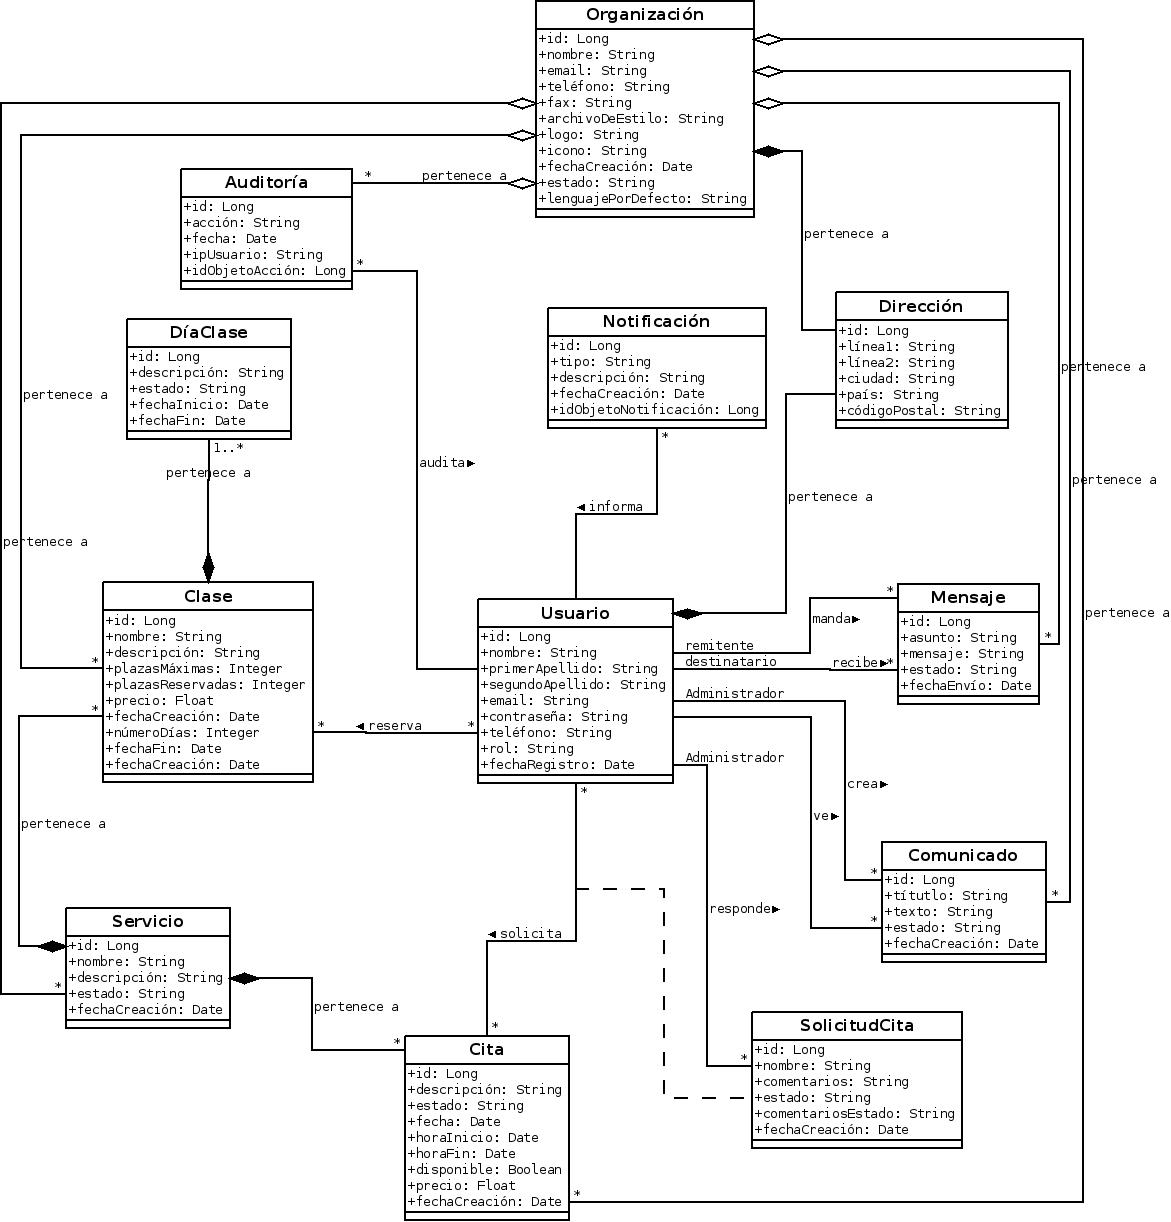
\includegraphics[scale=.35]{img/modelo-conceptual.jpeg}
  \caption{Modelo Conceptual de Clases UML}
  \label{fig:modelo-conceptual}
\end{figure}


\section{Modelo de Casos de Uso}

A continuación se describirán los principales casos de uso que se llevarán a cabo en el sistema, correspondientes a los requisitos funcionales listados anteriormente en el apartado \ref{subsec:requisitosfuncionales}. Estos casos de uso se pueden emplear como mecanismo para representar las interacciones entre los actores y el sistema:


\begin{table}[H]
  \begin{center}
    \begin{tabularx}{16.4cm}{|l|X|}
      \hline
      \textbf{UC-01} & \textbf{Seleccionar idioma}\\
      \hline
      \textbf{Descripción} & Cambiar el idioma en el que se muestra la aplicación.\\
      \hline
      \textbf{Actores} & Usuario, administrador o superadministrador.\\
      \hline
      \textbf{Precondiciones} & Ninguna.\\
      \hline
      \textbf{Postcondiciones} & El idioma de la aplicación se establecerá al que el usuario seleccione. Se establecerá este lenguaje por defecto para el usuario.\\
      \hline
      \textbf{Escenario principal} & \smallskip 1. El usuario selecciona uno de los idiomas disponibles en la lista de selección del mismo, en cualquier pantalla de la aplicación.\\
      & 2. La aplicación se mostrará en el idioma seleccionado.\\
      & 3. El idioma se establece por defecto para el resto de veces que el usuario acceda a la aplicación.\\
      & \\
      \hline
      \textbf{Escenarios alternativos} & \\
      & \\
      \hline
    \end{tabularx}
    \caption{UC-01: Seleccionar idioma}
    \label{tab:CU-idioma}
  \end{center}
\end{table}


\begin{table}[H]
  \begin{center}
    \begin{tabularx}{16.4cm}{|l|X|}
      \hline
      \textbf{UC-02} & \textbf{Registro}\\
      \hline
      \textbf{Descripción} & Registro de usuario en el sistema.\\
      \hline
      \textbf{Actores} & Usuario.\\
      \hline
      \textbf{Precondiciones} & El usuario no puede haberse registrado previamente.\\
      \hline
      \textbf{Postcondiciones} & El usuario quedará registrado en el sistema y se mostrará la página de inicio del mismo.\\
      \hline
      \textbf{Escenario principal} & \smallskip 1. El sistema muestra la página de registro con los campos correspondientes.\\
      & 2. El usuario rellena al menos los campos obligatorios y marca la casilla de aceptación de términos y condiciones. \\
      & 3. Una vez aceptado los términos y condiciones, el sistema habilita el botón de registro. \\ 
      & 4. El usuario hace click en el botón de registro.\\
      & 5. El sistema valida los datos y registra al usuario en la base de datos.\\
      & 6. El sistema realiza el login del usuario y lo redirige automáticamente a la página de inicio de la aplicación.\\
      & \\
      \hline
      \textbf{Escenarios alternativos} & \smallskip 5.a. Los datos introducidos no son válidos:\\
      & \hspace{0.3cm} 5.a.1. El sistema muestra el mensaje de error correspondiente.\\
      & \hspace{0.3cm} 5.a.2. Vuelve al paso 2.\\
      & \\
      \hline
    \end{tabularx}
    \caption{UC-02: Gestión de usuarios: Registro}
    \label{tab:CU-registro}
  \end{center}
\end{table}


\begin{table}
  \begin{center}
    \begin{tabularx}{16.4cm}{|l|X|}
      \hline
      \textbf{UC-03} & \textbf{Login}\\
      \hline
      \textbf{Descripción} & Inicio de sesión del usuario en el sistema.\\
      \hline
      \textbf{Actores} & Usuario, administrador o superadministrador.\\
      \hline
      \textbf{Precondiciones} & Ninguna.\\
      \hline
      \textbf{Postcondiciones} & El usuario se identificará en el sistema y se mostrará la página de inicio.\\
      \hline
      \textbf{Escenario principal} & \smallskip 1. El sistema muestra la pantalla de inicio de sesión.\\
      & 2. El usuario introduce su correo electrónico y contraseña.\\
      & 3. El sistema valida los datos e inicia la sesión del usuario.\\
      & 4. El sistema muestra la página de inicio con el menú principal.\\
      & \\
      \hline
      \textbf{Escenarios alternativos} & \smallskip 3.a. Los datos introducidos no son válidos:\\
      & \hspace{0.3cm} 3.a.1. El sistema muestra el mensaje de error correspondiente.\\
      & \hspace{0.3cm} 3.a.2. Vuelve al paso 2.\\
      & \\
      \hline
    \end{tabularx}
    \caption{UC-03: Gestión de usuarios: Login}
    \label{tab:CU-login}
  \end{center}
\end{table}


\begin{table}
  \begin{center}
    \begin{tabularx}{16.4cm}{|l|X|}
      \hline
      \textbf{UC-05} & \textbf{Restablecer contraseña}\\
      \hline
      \textbf{Descripción} & Restablecer la contraseña del usuario si esta ha sido olvidada.\\
      \hline
      \textbf{Actores} & Usuario, administrador o superadministrador.\\
      \hline
      \textbf{Precondiciones} & El usuario debe estar registrado en el sistema y su correo electrónico estar operativo.\\
      \hline
      \textbf{Postcondiciones} & El usuario establecerá una nueva contraseña para su login.\\
      \hline
      \textbf{Escenario principal} & \smallskip 1. El sistema muestra la pantalla de restablecer contraseña. \\
      & 2. El usuario introduce la dirección de correo electrónico que usó para su registro.\\
      & 3. El sistema valida la dirección y envía un correo con el enlace para restablecer la contraseña.\\
      & 4. El usuario accede al enlace recibido en el email.\\
      & 5. El usuario introduce su nueva contraseña y la repite por seguridad.\\
      & 6. El sistema valida los datos y la nueva contraseña para el usuario queda registrada en la base de datos.\\
      & \\
      \hline
      \textbf{Escenarios alternativos} & \smallskip  3.a. La dirección de correo introducida no es válida:\\
      & \hspace{0.3cm} 3.a.1. El sistema muestra el mensaje de error correspondiente.\\
      & \hspace{0.3cm} 3.a.2. Vuelve al paso 2.\\
      & 4.a. El correo electrónico no ha sido recibido:\\
      & \hspace{0.3cm} 4.a.1. Vuelve al paso 1.\\
      & 4.b. El enlace no es válido o ha expirado:\\
      & \hspace{0.3cm} 4.b.1. Vuelve al paso 1.\\
      & 6.a. Las contraseñas introducidas no son válidas:\\
      & \hspace{0.3cm} 6.a.1. El sistema muestra el mensaje de error correspondiente.\\
      & \hspace{0.3cm} 6.a.2. Vuelve al paso 5.\\
      & \\
      \hline
    \end{tabularx}
    \caption{UC-05: Gestión de usuarios: Recuperar contraseña}
    \label{tab:CU-restablecer-contrasena}
  \end{center}
\end{table}


\begin{table}[H]
  \begin{center}
    \begin{tabularx}{16.4cm}{|l|X|}
      \hline
      \textbf{UC-04} & \textbf{Cerrar sesión}\\
      \hline
      \textbf{Descripción} & Cerrar la sesión del usuario en el sistema.\\
      \hline
      \textbf{Actores} & Usuario, administrador o superadministrador.\\
      \hline
      \textbf{Precondiciones} & Debe ser un usuario previamente identificado.\\
      \hline
      \textbf{Postcondiciones} & Se terminará la sesión del usuario.\\
      \hline
      \textbf{Escenario principal} & \smallskip 1. El usuario hará click en la opción para salir del sistema desde cualquier pantalla de la aplicación.\\
      & 2. El sistema cerrará la sesión, quedando esta inhabilitada.\\
      & \\
      \hline
      \textbf{Escenarios alternativos} & \smallskip 1.a. El usuario hace click en salir del sistema a través del menú de opciones.\\
      & \\
      \hline
    \end{tabularx}
    \caption{UC-04: Gestión de usuarios: Cerrar sesión}
    \label{tab:CU-cerrar-sesion}
  \end{center}
\end{table}


\begin{table}
  \begin{center}
    \begin{tabularx}{16.4cm}{|l|X|}
      \hline
      \textbf{UC-06} & \textbf{Cambiar contraseña}\\
      \hline
      \textbf{Descripción} & Establecer una nueva contraseña para el usuario.\\
      \hline
      \textbf{Actores} & Usuario, administrador o superadministrador.\\
      \hline
      \textbf{Precondiciones} & El usuario debe haberse identificado previamente.\\
      \hline
      \textbf{Postcondiciones} & El usuario establecerá una nueva contraseña para su login.\\
      \hline
      \textbf{Escenario principal} & \smallskip 1. El sistema muestra la pantalla donde ingresar los datos para la nueva contraseña.\\
      & 2. El usuario introduce los datos pedidos.\\
      & 3. El sistema valida los datos y la nueva contraseña para el usuario queda registrada en la base de datos.\\
      & \\
      \hline
      \textbf{Escenarios alternativos} & \smallskip 3.a. Los datos introducidos no son válidos:\\
      & \hspace{0.3cm} 3.a.1. El sistema muestra el mensaje de error correspondiente.\\
      & \hspace{0.3cm} 3.a.2. Vuelve al paso 2.\\
      & \\
      \hline
    \end{tabularx}
    \caption{UC-06: Gestión de usuarios: Cambiar contraseña}
    \label{tab:CU-cambiar-contrasena}
  \end{center}
\end{table}


\begin{table}
  \begin{center}
    \begin{tabularx}{16.4cm}{|l|X|}
      \hline
      \textbf{UC-07} & \textbf{Editar perfil}\\
      \hline
      \textbf{Descripción} & Modificación de los datos del usuario.\\
      \hline
      \textbf{Actores} & Usuario, administrador o superadministrador..\\
      \hline
      \textbf{Precondiciones} & Debe ser un usuario previamente identificado en el sistema.\\
      \hline
      \textbf{Postcondiciones} & El usuario podrá modificar sus datos, excepto el email.\\
      \hline
      \textbf{Escenario principal} & \smallskip 1. El usuario navega hasta su perfil.\\
      & 2. El usuario hace click en la opción de editar. \\
      & 3. El sistema muestra los datos del perfil en campos editables.\\
      & 4. El usuario modifica o rellena los datos correspondientes.\\
      & 5. El sistema modifica los datos y muestra el mensaje del proceso completado.\\ 
      & \\
      \hline
      \textbf{Escenarios alternativos} & \smallskip 5.a. Los datos introducidos no son válidos:\\
      & \hspace{0.3cm} 5.a.1. El sistema muestra el mensaje de error correspondiente.\\
      & \hspace{0.3cm} 5.a.2. Vuelve al paso 4.\\
      & \\
      \hline
    \end{tabularx}
    \caption{UC-07: Gestión de usuarios: Editar perfil}
    \label{tab:CU-editar-perfil}
  \end{center}
\end{table}


\begin{table}
  \begin{center}
    \begin{tabularx}{16.4cm}{|l|X|}
      \hline
      \textbf{UC-08} & \textbf{Leer el correo interno}\\
      \hline
      \textbf{Descripción} & Leer alguno de los correos recibidos o enviados.\\
      \hline
      \textbf{Actores} & Usuario, administrador o superadministrador.\\
      \hline
      \textbf{Precondiciones} & El usuario debe haberse identificado previamente.\\
      \hline
      \textbf{Postcondiciones} & El sistema mostrará el mensaje seleccionado.\\
      \hline
      \textbf{Escenario principal} & \smallskip 1. El usuario navega hasta la página deseada donde se encuentra el correo a leer, ya sea recibido o enviado.\\
      & 2. El usuario hace click en el asunto del mensaje en cuestión.\\
      & 3. El sistema muestra el mensaje y sus datos correspondientes. Si el mensaje no había sido previamente abierto, se marcará como mensaje leído.\\
      & \\
      \hline
      \textbf{Escenarios alternativos} & \\
      & \\
      \hline
    \end{tabularx}
    \caption{UC-08: Gestión de servicios: Leer correo interno}
    \label{tab:CU-leer-correo}
  \end{center}
\end{table}


\begin{table}
  \begin{center}
    \begin{tabularx}{16.4cm}{|l|X|}
      \hline
      \textbf{UC-09} & \textbf{Mandar un correo}\\
      \hline
      \textbf{Descripción} & Mandar un correo interno a otro usuario de la aplicación.\\
      \hline
      \textbf{Actores} & Usuario, administrador o superadministrador.\\
      \hline
      \textbf{Precondiciones} & El usuario debe haberse identificado previamente.\\
      \hline
      \textbf{Postcondiciones} & Se mandará el mensaje redactado al usuario seleccionado.\\
      \hline
      \textbf{Escenario principal} & \smallskip 1. El sistema muestra la página para redactar un nuevo email.\\
      & 2. El usuario selecciona destinatario e introduce asunto y el mensaje a mandar.\\
      & 3. El sistema valida los datos y manda el correo a la persona seleccionada.\\
      & \\
      \hline
      \textbf{Escenarios alternativos} & \smallskip 3.a. Los datos introducidos no son válidos:\\
      & \hspace{0.3cm} 3.a.1. El sistema muestra el mensaje de error correspondiente.\\
      & \hspace{0.3cm} 3.a.2. Vuelve al paso 2.\\
      & \\
      \hline
    \end{tabularx}
    \caption{UC-09: Gestión de servicios: Mandar un correo}
    \label{tab:CU-mandar-correo}
  \end{center}
\end{table}


\begin{table}
  \begin{center}
    \begin{tabularx}{16.4cm}{|l|X|}
      \hline
      \textbf{UC-10} & \textbf{Notificaciones}\\
      \hline
      \textbf{Descripción} & Registro de notificaciones destinadas al usuario.\\
      \hline
      \textbf{Actores} & Usuario, administrador o superadministrador.\\
      \hline
      \textbf{Precondiciones} & Debe ser un usuario previamente identificado.\\
      \hline
      \textbf{Postcondiciones} & El sistema mostrará las notificaciones que se han generado para el usuario en las fechas indicadas.\\
      \hline
      \textbf{Escenario principal} & \smallskip 1. El sistema mostrará la página correspondiente al histórico de notificaciones.\\
      & 2. El usuario seleccionará el periodo en el que desea ver las notificaciones y el tipo de notificación si lo desea.\\
      & 3. El sistema muestra las notificaciones correspondientes.\\
      & \\
      \hline
      \textbf{Escenarios alternativos} & \\
      & \\
      \hline
    \end{tabularx}
    \caption{UC-10: Notificaciones}
    \label{tab:CU-notificaciones}
  \end{center}
\end{table}


\begin{table}[H]
  \begin{center}
    \begin{tabularx}{16.4cm}{|l|X|}
      \hline
      \textbf{UC-11} & \textbf{Reservar plaza en una clase}\\
      \hline
      \textbf{Descripción} & El usuario podrá reservar una plaza en una clase.\\
      \hline
      \textbf{Actores} & Usuario, administrador o superadministrador.\\
      \hline
      \textbf{Precondiciones} & El usuario debe haberse identificado previamente y debe haber alguna plaza libre en la clase.\\
      \hline
      \textbf{Postcondiciones} & El usuario tendrá una plaza reservada en una clase.\\
      \hline
      \textbf{Escenario principal} & \smallskip 1. El sistema muestra las clases disponibles con su información principal.\\
      & 2. El usuario hace clic en ver la información de la clase.\\
      & 3. El sistema muestra la página con los detalles de la clase.\\
      & 2. El usuario hace clic en la opción de reservar plaza.\\
      & 3. El sistema realiza la reserva y muestra el mensaje.\\
      & \\
      \hline
      \textbf{Escenarios alternativos} & \smallskip 2.a. La clase a solicitar no dispone de plazas libres.\\
      & \hspace{0.3cm} 2.a.1. El icono para solicitar plaza no se mostrará. \\
      & \\
      \hline
    \end{tabularx}
    \caption{UC-11: Gestión de servicios: Reservar plaza en una clase}
    \label{tab:CU-reservar-clase}
  \end{center}
\end{table}


\begin{table}
  \begin{center}
    \begin{tabularx}{16.4cm}{|l|X|}
      \hline
      \textbf{UC-12} & \textbf{Cancelación de reserva de una clase}\\
      \hline
      \textbf{Descripción} & El usuario cancelará la reserva de una clase, quedando así su plaza libre.\\
      \hline
      \textbf{Actores} & Usuario, administrador o superadministrador.\\
      \hline
      \textbf{Precondiciones} & El usuario debe haberse identificado previamente.\\
      \hline
      \textbf{Postcondiciones} & El usuario se dará de baja en una clase, quedando su plaza libre.\\
      \hline
      \textbf{Escenario principal} & \smallskip 1. El sistema mostrará las clases disponibles.\\
      & 2. El usuario hace clic en ver la información de la clase.\\
      & 3. El sistema muestra la información de la clase.\\
      & 4. El usuario hará click en la opción correspondiente para darse de baja de esa clase.\\
      & 5. El sistema dará de baja al usuario, quedando así su plaza libre en la clase. \\
      & \\
      \hline
      \textbf{Escenarios alternativos} & \\ 
      & \\
      \hline
    \end{tabularx}
    \caption{UC-12: Gestión de servicios: Cancelación de reserva de una clase}
    \label{tab:CU-cancelar-reserva-clase}
  \end{center}
\end{table}


\begin{table}
  \begin{center}
    \begin{tabularx}{16.4cm}{|l|X|}
      \hline
      \textbf{UC-13} & \textbf{Solicitar cita}\\
      \hline
      \textbf{Descripción} & El usuario podrá solicitar cita de un determinado servicio a la hora seleccionada.\\
      \hline
      \textbf{Actores} & Usuario y administrador o superadministrador.\\
      \hline
      \textbf{Precondiciones} & El usuario y administrador deben haberse identificado previamente.\\
      \hline
      \textbf{Postcondiciones} & Se le asignará la cita seleccionada al usuario.\\
      \hline
      \textbf{Escenario principal} & \smallskip 1. El sistema muestra las citas disponibles.\\
      & 2. El usuario selecciona la cita y envía la solicitud.\\
      & 3. El sistema marca la cita como pendiente y no estará disponible para el resto de usuarios. \\
      & 4. El sistema hace llegar la solicitud a los administradores.\\
      & 5. El administrador acepta la solicitud del usuario.\\
      & 6. El sistema registra la cita y manda una notificación de aceptación al usuario.\\
      & \\
      \hline
      \textbf{Escenarios alternativos} & \smallskip 3.a. El usuario es administrador o superadministrador:\\
      & \hspace{0.3cm} 3.a.1. El sistema marca la cita como aceptada y no estará disponible para el resto de usuarios. \\
      & \hspace{0.3cm} 3.a.2. El escenario acabaría en este punto.\\
      & \smallskip 5.a. El administrador declina la solicitud de cita del usuario:\\
      & \hspace{0.3cm} 5.a.1. El sistema envía una notificación al usuario.\\
      & \hspace{0.3cm} 5.a.2. Vuelve al punto 1.\\
      & \\
      \hline
    \end{tabularx}
    \caption{UC-13: Gestión de servicios: Solicitar cita}
    \label{tab:CU-solicitar-cita}
  \end{center}
\end{table}


\begin{table}[H]
  \begin{center}
    \begin{tabularx}{16.4cm}{|l|X|}
      \hline
      \textbf{UC-14} & \textbf{Responder a solicitud de cita}\\
      \hline
      \textbf{Descripción} & Respuesta de una solicitud de cita por parte del administrador o superadministrador. \\
      \hline
      \textbf{Actores} & Administrador o superadministrador.\\
      \hline
      \textbf{Precondiciones} & El administrador debe haberse identificado previamente.\\
      \hline
      \textbf{Postcondiciones} & La solicitud de cita del usuario quedará respondida.\\
      \hline
      \textbf{Escenario principal} & \smallskip 1. El sistema muestra el listado de citas.\\
      & 2. El administrador selecciona la cita que desea responder.\\
      & 3. El sistema muestra la información de la cita y opciones disponibles.\\
      & 4. El administrador selecciona la opción correspondiente (aceptar o rechazar la solicitud).\\
      & 5. El sistema registra la respuesta, y realiza los cambios oportunos en la cita, y notifica al usuario.\\
      & \\
      \hline
      \textbf{Escenarios alternativos} & \\
      & \\
      \hline
    \end{tabularx}
    \caption{UC-14: Gestión de servicios: Responder a solicitud de cita}
    \label{tab:CU-responder-solicitud-cita}
  \end{center}
\end{table}


\begin{table}
  \begin{center}
    \begin{tabularx}{16.4cm}{|l|X|}
      \hline
      \textbf{UC-15} & \textbf{Cancelar cita}\\
      \hline
      \textbf{Descripción} & Cancelación de una cita o solicitud de cita por parte del propio usuario. \\
      \hline
      \textbf{Actores} & Usuario, administrador o superadministrador..\\
      \hline
      \textbf{Precondiciones} & El usuario debe haberse identificado previamente.\\
      \hline
      \textbf{Postcondiciones} & La cita o solicitud de cita del usuario quedará cancelada.\\
      \hline
      \textbf{Escenario principal} & \smallskip 1. El sistema muestra el listado de citas.\\
      & 2. El usuario selecciona la cita que desea cancelar.\\
      & 3. El sistema muestra la información de la cita y opciones disponibles.\\
      & 4. El usuario selecciona cancelar la cita.\\
      & 5. El sistema cancela la cita dejándola libre nuevamente, y notifica a los administradores.\\
      & \\
      \hline
      \textbf{Escenarios alternativos} & \\
      & \\
      \hline
    \end{tabularx}
    \caption{UC-15: Gestión de servicios: Cancelar cita}
    \label{tab:CU-cancelar-cita}
  \end{center}
\end{table}


\begin{table}
  \begin{center}
    \begin{tabularx}{16.4cm}{|l|X|}
      \hline
      \textbf{UC-16} & \textbf{Cancelar cita de un usuario}\\
      \hline
      \textbf{Descripción} & Cancelación de una cita por parte del administrador. \\
      \hline
      \textbf{Actores} & Administrador o superadministrador..\\
      \hline
      \textbf{Precondiciones} & El usuario debe haberse identificado previamente como administrador.\\
      \hline
      \textbf{Postcondiciones} & La cita del usuario quedará cancelada por parte del administrador.\\
      \hline
      \textbf{Escenario principal} & \smallskip 1. El sistema muestra el listado de citas.\\
      & 2. El administrador selecciona la cita que desea cancelar.\\
      & 3. El sistema muestra la información de la cita y opciones disponibles.\\
      & 4. El administrador selecciona cancelar la cita.\\
      & 5. El sistema cancela la cita dejándola libre nuevamente y notifica al usuario.\\
      & \\
      \hline
      \textbf{Escenarios alternativos} & \\
      & \\
      \hline
    \end{tabularx}
    \caption{UC-16: Gestión de servicios: Cancelar cita de un usuario}
    \label{tab:CU-cancelar-cita-admin}
  \end{center}
\end{table}


\begin{table}
  \begin{center}
    \begin{tabularx}{16.4cm}{|l|X|}
      \hline
      \textbf{UC-17} & \textbf{Calendario de actividades}\\
      \hline
      \textbf{Descripción} & El usuario dispondrá de un calendario donde ver todas las clases y citas. \\
      \hline
      \textbf{Actores} & Usuario, administrador o superadministrador..\\
      \hline
      \textbf{Precondiciones} & El usuario debe haberse identificado previamente.\\
      \hline
      \textbf{Postcondiciones} & El sistema mostrará el calendario con las clases y citas del usuario.\\
      \hline
      \textbf{Escenario principal} & \smallskip 1. El usuario navegará hasta la página correspondiente del calendario.\\
      & 2. El sistema mostrará el calendario con los datos de actividades y citas de todos los servicios, distinguiendo por colores las pasadas, reservadas, disponibles o no disponibles.\\
      & \\
      \hline
      \textbf{Escenarios alternativos} & \\
      & \\
      \hline
    \end{tabularx}
    \caption{UC-17: Gestión de servicios: Calendario de actividades}
    \label{tab:CU-calendario}
  \end{center}
\end{table}


\begin{table}
  \begin{center}
    \begin{tabularx}{16.4cm}{|l|X|}
      \hline
      \textbf{UC-18} & \textbf{Consultar mis reservas}\\
      \hline
      \textbf{Descripción} & El usuario, administrador o superadministrador podrá ver la lista de sus clases y citas reservadas o pendientes. \\
      \hline
      \textbf{Actores} & Usuario, administrador o superadministrador. \\
      \hline
      \textbf{Precondiciones} & El usuario debe haberse identificado previamente.\\
      \hline
      \textbf{Postcondiciones} & El sistema mostrará el todas las clases y citas del usuario.\\
      \hline
      \textbf{Escenario principal} & \smallskip 1. El usuario navegará hasta la página correspondiente de reservas realizadas.\\
      & 2. El sistema mostrará la lista de clases y citas de todos los servicios que el usuario haya reservado.\\
      & \\
      \hline
      \textbf{Escenarios alternativos} & \\
      & \\
      \hline
    \end{tabularx}
    \caption{UC-18: Gestión de servicios: Consultar mis reservas}
    \label{tab:CU-reservas}
  \end{center}
\end{table}


\begin{table}
  \begin{center}
    \begin{tabularx}{16.4cm}{|l|X|}
      \hline
      \textbf{UC-19} & \textbf{Auditoría}\\
      \hline
      \textbf{Descripción} & Registro de operaciones llevadas a cabo en el sistema por el usuario.\\
      \hline
      \textbf{Actores} & Usuario.\\
      \hline
      \textbf{Precondiciones} & Debe ser un usuario previamente identificado.\\
      \hline
      \textbf{Postcondiciones} & El sistema mostrará las acciones llevadas a cabo por el usuario en las fechas indicadas.\\
      \hline
      \textbf{Escenario principal} & \smallskip 1. El sistema mostrará la página correspondiente al histórico de acciones.\\
      & 2. El usuario seleccionará el periodo del que desea ver las acciones llevadas a cabo y el tipo de acción si lo desea.\\
      & 3. El sistema muestra las acciones correspondientes.\\
      & \\
      \hline
      \textbf{Escenarios alternativos} & \\
      & \\
      \hline
    \end{tabularx}
    \caption{UC-19: Auditoría}
    \label{tab:CU-auditorias}
  \end{center}
\end{table}


\begin{table}
  \begin{center}
    \begin{tabularx}{16.4cm}{|l|X|}
      \hline
      \textbf{UC-20} & \textbf{Auditoría para administradores}\\
      \hline
      \textbf{Descripción} & Registro de operaciones llevadas a cabo en el sistema por el administrador o los usuarios.\\
      \hline
      \textbf{Actores} & Administrador o superadministrador.\\
      \hline
      \textbf{Precondiciones} & Debe ser un usuario previamente identificado como administrador o superadministrador.\\
      \hline
      \textbf{Postcondiciones} & El sistema mostrará las acciones llevadas a cabo por el el propio administrador o un usuario seleccionado en las fechas indicadas.\\
      \hline
      \textbf{Escenario principal} & \smallskip 1. El sistema mostrará la página correspondiente al histórico de acciones.\\
      & 2. El administrador seleccionará el periodo del que desea ver las acciones llevadas a cabo, así como el usuario y el tipo de acción si lo desea.\\
      & 3. El sistema muestra las acciones correspondientes.\\
      & \\
      \hline
      \textbf{Escenarios alternativos} & \\
      & \\
      \hline
    \end{tabularx}
    \caption{UC-20: Auditoría para administradores}
    \label{tab:CU-auditorias-admin}
  \end{center}
\end{table}


\begin{table}
  \begin{center}
    \begin{tabularx}{16.4cm}{|l|X|}
      \hline
      \textbf{UC-21} & \textbf{Activar o suspender usuario}\\
      \hline
      \textbf{Descripción} & Activar o suspender a un usuario específico.\\
      \hline
      \textbf{Actores} & Administrador o superadministrador.\\
      \hline
      \textbf{Precondiciones} & Debe ser un usuario previamente identificado como administrador o superadministrador.\\
      \hline
      \textbf{Postcondiciones} & El administrador podrá suspender o activar el usuario seleccionado.\\
      \hline
      \textbf{Escenario principal} & \smallskip 1. El sistema muestra el listado de usuarios del sistema.\\
      & 2. El administrador navega por la lista y selecciona la acción correspondiente en la casilla del usuario en cuestión.\\
      & 3. El sistema ejecuta la acción seleccionada (activar/suspender).\\
      & \\
      \hline
      \textbf{Escenarios alternativos} & \\
      & \\
      \hline
    \end{tabularx}
    \caption{UC-21: Gestión de usuarios: Activar o suspender}
    \label{tab:CU-activar-suspender-usuario}
  \end{center}
\end{table}


\begin{table}[H]
  \begin{center}
    \begin{tabularx}{16.4cm}{|l|X|}
      \hline
      \textbf{UC-22} & \textbf{Ver perfil}\\
      \hline
      \textbf{Descripción} & Los administrador podrán ver el perfil de los usuarios del sistema.\\
      \hline
      \textbf{Actores} & Administrador o superadministrador.\\
      \hline
      \textbf{Precondiciones} & Debe ser un usuario previamente identificado como administrador o superadministrador.\\
      \hline
      \textbf{Postcondiciones} & El administrador podrá ver el perfil del usuario seleccionado.\\
      \hline
      \textbf{Escenario principal} & \smallskip 1. El sistema muestra el listado de usuarios del sistema.\\
      & 2. El administrador navega por la lista y selecciona la acción del usuario en cuestión.\\
      & 3. El sistema redirecciona al administrador a la página del perfil del usuario.\\
      & \\
      \hline
      \textbf{Escenarios alternativos} & \\
      & \\
      \hline
    \end{tabularx}
    \caption{UC-22: Gestión de usuarios: Ver perfil}
    \label{tab:CU-ver-perfil-admin}
  \end{center}
\end{table}


\begin{table}
  \begin{center}
    \begin{tabularx}{16.4cm}{|l|X|}
      \hline
      \textbf{UC-23} & \textbf{Editar usuario}\\
      \hline
      \textbf{Descripción} & Modificación de los datos de usuarios por parte del administrador.\\
      \hline
      \textbf{Actores} & Administrador o superadministrador.\\
      \hline
      \textbf{Precondiciones} & Debe ser un usuario previamente identificado como administrador o superadministrador.\\
      \hline
      \textbf{Postcondiciones} & El administrador podrá modificar los datos del usuario seleccionado.\\
      \hline
      \textbf{Escenario principal} & \smallskip 1. El administrador se dirige al perfil del usuario deseado siguiendo los pasos de gestión de usuario detallados en el caso de uso anterior.\\
      & 2. El administrador hace click en la opción de modificar usuario. \\
      & 3. El sistema muestra los datos del usuario en campos editables.\\
      & 4. El administrador modifica o rellena los datos correspondientes.\\
      & 5. El sistema modifica los datos y notifica al usuario de los cambios realizados.\\ 
      & \\
      \hline
      \textbf{Escenarios alternativos} & \smallskip 5.a. Los datos introducidos no son válidos:\\
      & \hspace{0.3cm} 5.a.1. El sistema muestra el mensaje de error correspondiente.\\
      & \hspace{0.3cm} 5.a.2. Vuelve al paso 4.\\
      & \\
      \hline
    \end{tabularx}
    \caption{UC-23: Gestión de usuarios: Editar usuario}
    \label{tab:CU-editar-usuario-admin}
  \end{center}
\end{table}


\begin{table}
  \begin{center}
    \begin{tabularx}{16.4cm}{|l|X|}
      \hline
      \textbf{UC-24} & \textbf{Ver administrador}\\
      \hline
      \textbf{Descripción} & Ver perfil de administradores. \\
      \hline
      \textbf{Actores} & Administrador o superadministrador.\\
      \hline
      \textbf{Precondiciones} & Debe ser un usuario previamente identificado como administrador o superadministrador.\\
      \hline
      \textbf{Postcondiciones} & El administrador podrá ver los datos de otro administrador.\\
      \hline
      \textbf{Escenario principal} & \smallskip 1. El sistema muestra el listado de administradores del sistema.\\
      & 2. El administrador navega por la lista y selecciona la acción correspondiente en la casilla del administrador en cuestión.\\
      & 3. El sistema redirecciona al administrador a la página correspondiente al perfil del usuario.\\
      & \\
      \hline
      \textbf{Escenarios alternativos} & \\
      & \\
      \hline
    \end{tabularx}
    \caption{UC-24: Gestión de administradores: Ver perfil de administradores}
    \label{tab:CU-ver-perfil-de-admin}
  \end{center}
\end{table}


\begin{table}
  \begin{center}
    \begin{tabularx}{16.4cm}{|l|X|}
      \hline
      \textbf{UC-25} & \textbf{Activar o suspender administrador}\\
      \hline
      \textbf{Descripción} & Activar o suspender administrador por parte del superadministrador. \\
      \hline
      \textbf{Actores} & Superadministrador.\\
      \hline
      \textbf{Precondiciones} & Debe ser un usuario previamente identificado como superadministrador.\\
      \hline
      \textbf{Postcondiciones} & El superadministrador podrá activar/suspender al administrador seleccionado.\\
      \hline
      \textbf{Escenario principal} & \smallskip 1. El sistema muestra el listado de administradores del sistema.\\
      & 2. El superadministrador navega por la lista y selecciona la acción correspondiente en la casilla del administrador en cuestión.\\
      & 3. El sistema ejecuta la acción (activar/suspender) y refleja el nuevo estado del administrador en la lista. \\
      & \\
      \hline
      \textbf{Escenarios alternativos} & \\
      & \\
      \hline
    \end{tabularx}
    \caption{UC-25: Gestión de administradores: Activar o suspender administrador}
    \label{tab:CU-activar-suspender-admin}
  \end{center}
\end{table}


\begin{table}[H]
  \begin{center}
    \begin{tabularx}{16.4cm}{|l|X|}
      \hline
      \textbf{UC-26} & \textbf{Editar administrador}\\
      \hline
      \textbf{Descripción} & Modificación de los datos de administradores.\\
      \hline
      \textbf{Actores} & Superadministrador.\\
      \hline
      \textbf{Precondiciones} & Debe ser un usuario previamente identificado como superadministrador.\\
      \hline
      \textbf{Postcondiciones} & El superadministrador podrá modificar los datos del administrador seleccionado.\\
      \hline
      \textbf{Escenario principal} & \smallskip 1. El superadministrador se dirige al perfil del usuario deseado siguiendo los pasos de gestión de administrador detallados en el caso de uso correspondiente.\\
      & 2. El superadministrador hace click en la opción de editar. \\
      & 3. El sistema muestra los datos del administrador en campos editables.\\
      & 4. El superadministrador modifica o rellena los datos correspondientes.\\
      & 5. El sistema modifica los datos y notifica al administrador de los cambios realizados.\\ 
      & \\
      \hline
      \textbf{Escenarios alternativos} & \smallskip 5.a. Los datos introducidos no son válidos:\\
      & \hspace{0.3cm} 5.a.1. El sistema muestra el mensaje de error correspondiente.\\
      & \hspace{0.3cm} 5.a.2. Vuelve al paso 4.\\
      & \\
      \hline
    \end{tabularx}
    \caption{UC-26: Gestión de administradores: Editar administrador}
    \label{tab:CU-editar-admin}
  \end{center}
\end{table}


\begin{table}
  \begin{center}
    \begin{tabularx}{16.4cm}{|l|X|}
      \hline
      \textbf{UC-27} & \textbf{Alta de servicio}\\
      \hline
      \textbf{Descripción} & Añadir un servicio nuevo al sistema.\\
      \hline
      \textbf{Actores} & Administrador o superadministrador.\\
      \hline
      \textbf{Precondiciones} & Debe ser un usuario previamente identificado como administrador o superadministrador.\\
      \hline
      \textbf{Postcondiciones} & Se añadirá un nuevo servicio al sistema.\\
      \hline
      \textbf{Escenario principal} & \smallskip 1. El sistema muestra la lista de servicios actuales.\\
      & 2. El administrador hace click en la opción de añadir un nuevo servicio.\\
      & 3. El sistema muestra una ventana con los datos necesarios para la creación del servicio.\\
      & 4. El administrador introduce los datos necesarios.\\
      & 5. El sistema valida los datos y registra el nuevo servicio, quedando reflejado en la lista.\\
      & \\
      \hline
      \textbf{Escenarios alternativos} & \smallskip 5.a. Los datos introducidos no son válidos:\\
      & \hspace{0.3cm} 5.a.1. El sistema muestra el mensaje de error correspondiente.\\
      & \hspace{0.3cm} 5.a.2. Vuelve al paso 4.\\
      & \\
      \hline
    \end{tabularx}
    \caption{UC-27: Gestión de servicios: Alta de servicio}
    \label{tab:CU-alta-servicio}
  \end{center}
\end{table}




\begin{table}
  \begin{center}
    \begin{tabularx}{16.4cm}{|l|X|}
      \hline
      \textbf{UC-29} & \textbf{Editar servicio}\\
      \hline
      \textbf{Descripción} & Editar uno de los servicios del sistema.\\
      \hline
      \textbf{Actores} & Administrador o superadministrador.\\
      \hline
      \textbf{Precondiciones} & Debe ser un usuario previamente identificado como administrador o superadministrador.\\
      \hline
      \textbf{Postcondiciones} & El administrador editará los datos de unos de los servicios existentes en el sistema.\\
      \hline
      \textbf{Escenario principal} & \smallskip 1. El sistema muestra la lista de servicios actuales.\\
      & 2. El administrador hace click en la opción de editar de la casilla del servicio deseado.\\
      & 3. El sistema muestra una ventana editable con los datos actuales del servicio.\\
      & 4. El administrador edita los datos deseados.\\
      & 5. El sistema valida los datos y registra los cambios, quedando reflejados en la lista de servicios.\\
      & \\
      \hline
      \textbf{Escenarios alternativos} & \smallskip 5.a. Los datos introducidos no son válidos:\\
      & \hspace{0.3cm} 5.a.1. El sistema muestra el mensaje de error correspondiente.\\
      & \hspace{0.3cm} 5.a.2. Vuelve al paso 4.\\
      & \\
      \hline
    \end{tabularx}
    \caption{UC-29: Gestión de servicios: Editar servicio}
    \label{tab:CU-editar-servicio}
  \end{center}
\end{table}


\begin{table}
  \begin{center}
    \begin{tabularx}{16.4cm}{|l|X|}
      \hline
      \textbf{UC-30} & \textbf{Alta de clase}\\
      \hline
      \textbf{Descripción} & Añadir una clase nueva al sistema. A partir de este momento, los usuarios podrán reservar plaza en esta actividad.\\
      \hline
      \textbf{Actores} & Administrador o superadministrador.\\
      \hline
      \textbf{Precondiciones} & Debe ser un usuario previamente identificado como administrador o superadministrador.\\
      \hline
      \textbf{Postcondiciones} & Se añadirá una nueva clase del servicio seleccionado al sistema.\\
      \hline
      \textbf{Escenario principal} & \smallskip 1. El sistema muestra la lista de clases actuales.\\
      & 2. El administrador hace click en la opción de añadir una nueva clase.\\
      & 3. El sistema muestra una nueva página con los datos necesarios para la creación de la clase.\\
      & 4. El administrador introduce los datos necesarios.\\
      & 5. El sistema valida los datos y registra la clase.\\
      & \\
      \hline
      \textbf{Escenarios alternativos} & \smallskip 5.a. Los datos introducidos no son válidos:\\
      & \hspace{0.3cm} 5.a.1. El sistema muestra el mensaje de error correspondiente.\\
      & \hspace{0.3cm} 5.a.2. Vuelve al paso 4.\\
      & \\
      \hline
    \end{tabularx}
    \caption{UC-30: Gestión de servicios: Alta de clase}
    \label{tab:CU-alta-clase}
  \end{center}
\end{table}


\begin{table}
  \begin{center}
    \begin{tabularx}{16.4cm}{|l|X|}
      \hline
      \textbf{UC-31} & \textbf{Activar o suspender clase}\\
      \hline
      \textbf{Descripción} & Suspender o activar uno de las clases de un determinado servicio del sistema.\\
      \hline
      \textbf{Actores} & Administrador o superadministrador.\\
      \hline
      \textbf{Precondiciones} & Debe ser un usuario previamente identificado como administrador o superadministrador.\\
      \hline
      \textbf{Postcondiciones} & El administrador activará o suspenderá una de las clase existentes en el sistema.\\
      \hline
      \textbf{Escenario principal} & \smallskip 1. El sistema muestra la lista de clases actuales.\\
      & 2. El administrador hace click en la opción deseada (suspender/activar) de la casilla de la clase específica.\\
      & 3. El sistema suspende/activa la clase y notifica a los usuarios que estén haciendo uso de la misma sobre la acción.\\
      & \\
      \hline
      \textbf{Escenarios alternativos} & \smallskip \\
      & \\
      \hline
    \end{tabularx}
    \caption{UC-31: Gestión de servicios: Activar o suspender clase}
    \label{tab:CU-activar-suspender-clase}
  \end{center}
\end{table}


\begin{table}
  \begin{center}
    \begin{tabularx}{16.4cm}{|l|X|}
      \hline
      \textbf{UC-32} & \textbf{Editar clase}\\
      \hline
      \textbf{Descripción} & Editar uno de las clases del sistema.\\
      \hline
      \textbf{Actores} & Administrador o superadministrador.\\
      \hline
      \textbf{Precondiciones} & Debe ser un usuario previamente identificado como administrador o superadministrador.\\
      \hline
      \textbf{Postcondiciones} & El administrador editará los datos de una de las clase existentes en el sistema.\\
      \hline
      \textbf{Escenario principal} & \smallskip 1. El sistema muestra la lista de clases actuales.\\
      & 2. El administrador hace click en la opción de editar de la casilla de la clase deseada.\\
      & 3. El sistema muestra la página de edición de la clase con los datos actuales de la misma.\\
      & 4. El administrador edita los datos deseados.\\
      & 5. El sistema valida los datos y registra los cambios.\\
      & \\
      \hline
      \textbf{Escenarios alternativos} & \smallskip 5.a. Los datos introducidos no son válidos:\\
      & \hspace{0.3cm} 5.a.1. El sistema muestra el mensaje de error correspondiente.\\
      & \hspace{0.3cm} 5.a.2. Vuelve al paso 4.\\
      & \\
      \hline
    \end{tabularx}
    \caption{UC-32: Gestión de servicios: Editar clase}
    \label{tab:CU-editar-clase}
  \end{center}
\end{table}


\begin{table}
  \begin{center}
    \begin{tabularx}{16.4cm}{|l|X|}
      \hline
      \textbf{UC-33} & \textbf{Alta de cita}\\
      \hline
      \textbf{Descripción} & Añadir una cita al sistema para un determinado servicio.\\
      \hline
      \textbf{Actores} & Administrador o superadministrador.\\
      \hline
      \textbf{Precondiciones} & Debe ser un usuario previamente identificado como administrador o superadministrador.\\
      \hline
      \textbf{Postcondiciones} & Se añadirá al sistema una nueva cita del servicio seleccionado.\\
      \hline
      \textbf{Escenario principal} & \smallskip 1. El sistema muestra la lista de citas actuales.\\
      & 2. El administrador hace click en la opción de añadir una nueva cita.\\
      & 3. El sistema navega hacia la página de creación de una cita nueva.\\
      & 4. El administrador introduce los datos necesarios.\\
      & 5. El sistema valida los datos y registra la nueva cita, quedando disponible para su solicitud.\\
      & \\
      \hline
      \textbf{Escenarios alternativos} & \smallskip 5.a. Los datos introducidos no son válidos:\\
      & \hspace{0.3cm} 5.a.1. El sistema muestra el mensaje de error correspondiente.\\
      & \hspace{0.3cm} 5.a.2. Vuelve al paso 4.\\
      & \\
      \hline
    \end{tabularx}
    \caption{UC-33: Gestión de servicios: Alta de cita}
    \label{tab:CU-alta-cita}
  \end{center}
\end{table}


\begin{table}[H]
  \begin{center}
    \begin{tabularx}{16.4cm}{|l|X|}
      \hline
      \textbf{UC-28} & \textbf{Activar o suspender servicio}\\
      \hline
      \textbf{Descripción} & Activar o suspender uno de los servicios del sistema.\\
      \hline
      \textbf{Actores} & Administrador o superadministrador.\\
      \hline
      \textbf{Precondiciones} & Debe ser un usuario previamente identificado como administrador o superadministrador.\\
      \hline
      \textbf{Postcondiciones} & El administrador activará o suspenderá unos de los servicios existentes en el sistema.\\
      \hline
      \textbf{Escenario principal} & \smallskip 1. El sistema muestra la lista de servicios actuales.\\
      & 2. El administrador hace click en la opción deseada (suspender/activar) de la casilla del servicio específico.\\
      & 3. El sistema suspende/activa el servicio.\\
      & \\
      \hline
      \textbf{Escenarios alternativos} & \smallskip 3.a. Hay clases o citas pertenecientes al servicio a suspender.\\
      & \hspace{0.3cm} 3.a.1. El sistema muestra el mensaje de error correspondiente.\\
      & \hspace{0.3cm} 3.a.2. Vuelve al paso 2.\\      
      & \\
      \hline
    \end{tabularx}
    \caption{UC-28: Gestión de servicios: Activar o suspender servicio}
    \label{tab:CU-activar-suspender-servicio}
  \end{center}
\end{table}


\begin{table}
  \begin{center}
    \begin{tabularx}{16.4cm}{|l|X|}
      \hline
      \textbf{UC-34} & \textbf{Activar o suspender cita}\\
      \hline
      \textbf{Descripción} & Activar o suspender una de las citas de un determinado servicio del sistema.\\
      \hline
      \textbf{Actores} & Administrador o superadministrador.\\
      \hline
      \textbf{Precondiciones} & Debe ser un usuario previamente identificado como administrador o superadministrador.\\
      \hline
      \textbf{Postcondiciones} & El administrador activará o suspenderá una cita existente en el sistema.\\
      \hline
      \textbf{Escenario principal} & \smallskip 1. El sistema muestra la lista de citas actuales.\\
      & 2. El administrador hace click en la opción deseada (suspender/activar) de la cita específica.\\
      & 3. El sistema suspende/activa la cita, quedando esta inhabilitada/habilitada.\\
      & 4. En caso de ser una cita con usuario asignado, se le notificará el cambio al mismo.\\
      & \\
      \hline
      \textbf{Escenarios alternativos} & \smallskip \\
      & \\
      \hline
    \end{tabularx}
    \caption{UC-34: Gestión de servicios: Activar o suspender cita}
    \label{tab:CU-activar-suspender-cita}
  \end{center}
\end{table}


\begin{table}[H]
  \begin{center}
    \begin{tabularx}{16.4cm}{|l|X|}
      \hline
      \textbf{UC-35} & \textbf{Editar cita}\\
      \hline
      \textbf{Descripción} & Editar una cita del sistema.\\
      \hline
      \textbf{Actores} & Administrador o superadministrador.\\
      \hline
      \textbf{Precondiciones} & Debe ser un usuario previamente identificado como administrador o superadministrador.\\
      \hline
      \textbf{Postcondiciones} & El administrador editará los datos de una cita existente en el sistema.\\
      \hline
      \textbf{Escenario principal} & \smallskip 1. El sistema muestra la lista de citas actuales.\\
      & 2. El administrador hace click en la opción de editar en la cita deseada.\\
      & 3. El sistema navega hacia la página de edición de la cita seleccionada.\\
      & 4. El administrador edita los datos deseados.\\
      & 5. El sistema valida los datos y registra los cambios.\\
      & 6. En caso de ser una cita con usuario asignado, se le notificará el cambio al mismo.\\
      & \\
      \hline
      \textbf{Escenarios alternativos} & \smallskip 5.a. Los datos introducidos no son válidos:\\
      & \hspace{0.3cm} 5.a.1. El sistema muestra el mensaje de error correspondiente.\\
      & \hspace{0.3cm} 5.a.2. Vuelve al paso 4.\\
      & \\
      \hline
    \end{tabularx}
    \caption{UC-35: Gestión de servicios: Editar cita}
    \label{tab:CU-editar-cita}
  \end{center}
\end{table}


\begin{table}
  \begin{center}
    \begin{tabularx}{16.4cm}{|l|X|}
      \hline
      \textbf{UC-36} & \textbf{Subir archivo}\\
      \hline
      \textbf{Descripción} & Subir un archivo específico destinado a uno o varios usuarios, como entrenamientos personales, dietas, etc. \\
      \hline
      \textbf{Actores} & Administrador o superadministrador.\\
      \hline
      \textbf{Precondiciones} & Debe ser un usuario previamente identificado como administrador o superadministrador.\\
      \hline
      \textbf{Postcondiciones} & El administrador podrá subir un archivo especificando a qué usuario o usuarios va destinado el mismo, pero que este/estos puedan descargarlo.\\
      \hline
      \textbf{Escenario principal} & \smallskip 1. El sistema muestra la lista de documentos actuales.\\
      & 2. El administrador hace click en la opción de añadir un nuevo archivo.\\
      & 3. El sistema navega hacia la página de subida de archivos.\\
      & 4. El administrador introduce los datos necesarios, junto a los usuarios a los que van destinados el archivo, y selecciona el documento a subir de su dispositivo.\\
      & 5. El sistema valida los datos y aloja el archivo, quedando disponible para su descarga por los usuarios especificados.\\
      & \\
      \hline
      \textbf{Escenarios alternativos} & \\
      & \\
      \hline
    \end{tabularx}
    \caption{UC-36: Gestión de servicios: Subir archivo}
    \label{tab:CU-subir-archivo}
  \end{center}
\end{table}


\begin{table}
  \begin{center}
    \begin{tabularx}{16.4cm}{|l|X|}
      \hline
      \textbf{UC-38} & \textbf{Editar archivo}\\
      \hline
      \textbf{Descripción} & Editar los datos un archivo específico subido por un administrador, como entrenamientos personales, dietas, etc. \\
      \hline
      \textbf{Actores} & Administrador o superadministrador.\\
      \hline
      \textbf{Precondiciones} & Debe ser un usuario previamente identificado como administrador.\\
      & Debe haber algún documento subido.\\
      \hline
      \textbf{Postcondiciones} & El administrador podrá editar un archivo previamente subido.\\
      \hline
      \textbf{Escenario principal} & \smallskip 1. El sistema muestra el listado de archivos subidos.\\
      & 2. El administrador hace click en la opción de editar en el archivo deseado.\\
      & 3. El sistema navega hacia la página de edición del archivo seleccionado.\\
      & 4. El administrador edita los datos deseados.\\
      & 5. El sistema valida los datos y registra los cambios.\\
      & 6. En caso de ser una archivo con usuario/s asignado/s, se le/s notificará la edición del documento.\\
      & \\
      \hline
      \textbf{Escenarios alternativos} & \\
      & \\
      \hline
    \end{tabularx}
    \caption{UC-38: Gestión de servicios: Editar archivo}
    \label{tab:CU-editar-archivo}
  \end{center}
\end{table}


\begin{table}
  \begin{center}
    \begin{tabularx}{16.4cm}{|l|X|}
      \hline
      \textbf{UC-39} & \textbf{Eliminar archivo}\\
      \hline
      \textbf{Descripción} & Eliminar un archivo específico subido por un administrador, como entrenamientos personales, dietas, etc. \\
      \hline
      \textbf{Actores} & Administrador o superadministrador.\\
      \hline
      \textbf{Precondiciones} & Debe ser un usuario previamente identificado como administrador.\\
      & Debe haber algún documento subido.\\
      \hline
      \textbf{Postcondiciones} & El administrador podrá eliminar un archivo previamente subido.\\
      \hline
      \textbf{Escenario principal} & \smallskip 1. El sistema muestra el listado de archivos subidos.\\
      & 2. El administrador hace click en la opción de eliminar en el archivo deseado.\\
      & 3. El sistema elimina el documento.\\
      & 4. En caso de ser una archivo con usuario/s asignado/s, se le/s notificará la eliminación del documento.\\
      & \\
      \hline
      \textbf{Escenarios alternativos} & \\
      & \\
      \hline
    \end{tabularx}
    \caption{UC-39: Gestión de servicios: Eliminar archivo}
    \label{tab:CU-eliminar-archivo}
  \end{center}
\end{table}


\begin{table}[H]
  \begin{center}
    \begin{tabularx}{16.4cm}{|l|X|}
      \hline
      \textbf{UC-37} & \textbf{Descargar archivo}\\
      \hline
      \textbf{Descripción} & Descargar un archivo específico subido por un administrador, como entrenamientos personales, dietas, etc. \\
      \hline
      \textbf{Actores} & Usuario, administrador o superadministrador.\\
      \hline
      \textbf{Precondiciones} & Debe ser un usuario previamente identificado.\\
      & Debe haber algún documento subido destinado al usuario.\\
      \hline
      \textbf{Postcondiciones} & El usuario podrá descargar un archivo previamente subido por un administrador y destinado al mismo.\\
      \hline
      \textbf{Escenario principal} & \smallskip 1. El sistema muestra el listado de archivos disponibles para el usuario.\\
      & 2. El usuario selecciona el documento a descargar.\\
      & 3. El sistema realiza la descarga del mismo al dispositivo del usuario.\\
      & \\
      \hline
      \textbf{Escenarios alternativos} & \\
      & \\
      \hline
    \end{tabularx}
    \caption{UC-37: Gestión de servicios: Descargar archivo}
    \label{tab:CU-descargar-archivo}
  \end{center}
\end{table}


\begin{table}
  \begin{center}
    \begin{tabularx}{16.4cm}{|l|X|}
      \hline
      \textbf{UC-40} & \textbf{Nuevo comunicado}\\
      \hline
      \textbf{Descripción} & Los administradores podrán añadir comunicados o noticias que aparecerán en la página de inicio de los usuarios. \\
      \hline
      \textbf{Actores} & Administrador o superadministrador.\\
      \hline
      \textbf{Precondiciones} & El usuario debe haberse identificado previamente como administrador o superadministrador..\\
      \hline
      \textbf{Postcondiciones} & El administrador creará comunicados que serán visualizados por los usuarios al identificarse en el sistema. \\
      \hline
      \textbf{Escenario principal} & \smallskip 1. El sistema mostrará la página correspondiente al listado de comunicados existentes.\\
      & 2. El administrador selecciona la opción de crear un nuevo comunicado. \\
      & 3. El sistema muestra una nueva página con los datos necesarios para la creación del comunicado.\\
      & 4. El administrador introduce todos los datos.\\
      & 5. El sistema valida los datos y registra el comunicado, quedando visible para los usuarios.\\
      & \\
      \hline
      \textbf{Escenarios alternativos} & \\
      & \\
      \hline
    \end{tabularx}
    \caption{UC-40: Nuevo cominucado}
    \label{tab:CU-nuevo-comunicado}
  \end{center}
\end{table}


\begin{table}
  \begin{center}
    \begin{tabularx}{16.4cm}{|l|X|}
      \hline
      \textbf{UC-41} & \textbf{Activar o suspender comunicado}\\
      \hline
      \textbf{Descripción} & Activar o suspender uno de los comunicados del sistema.\\
      \hline
      \textbf{Actores} & Administrador o superadministrador.\\
      \hline
      \textbf{Precondiciones} & Debe ser un usuario previamente identificado como administrador o superadministrador.\\
      \hline
      \textbf{Postcondiciones} & El administrador activará o suspenderá una cita existente en el sistema.\\
      \hline
      \textbf{Escenario principal} & \smallskip 1. El sistema muestra la lista de comunicados actuales.\\
      & 2. El administrador hace click en la opción deseada (suspender/activar) del comunicado específico.\\
      & 3. El sistema suspende/activa el comunicado, quedando este inhabilitado/habilitado.\\
      & \\
      \hline
      \textbf{Escenarios alternativos} & \smallskip \\
      & \\
      \hline
    \end{tabularx}
    \caption{UC-41: Activar o suspender comunicado}
    \label{tab:CU-activar-suspender-comunicado}
  \end{center}
\end{table}


\begin{table}
  \begin{center}
    \begin{tabularx}{16.4cm}{|l|X|}
      \hline
      \textbf{UC-42} & \textbf{Editar comunicado}\\
      \hline
      \textbf{Descripción} & Editar un comunicado del sistema.\\
      \hline
      \textbf{Actores} & Administrador o superadministrador.\\
      \hline
      \textbf{Precondiciones} & Debe ser un usuario previamente identificado como administrador o superadministrador.\\
      \hline
      \textbf{Postcondiciones} & El administrador editará los datos de un comunicado existente en el sistema.\\
      \hline
      \textbf{Escenario principal} & \smallskip 1. El sistema muestra la lista de comunicados actuales.\\
      & 2. El administrador hace click en la opción de editar en el comunicado deseado.\\
      & 3. El sistema navega hacia la página de edición del comunicado seleccionada.\\
      & 4. El administrador edita los datos deseados.\\
      & 5. El sistema valida los datos y registra los cambios.\\
      & \\
      \hline
      \textbf{Escenarios alternativos} & \smallskip 5.a. Los datos introducidos no son válidos:\\
      & \hspace{0.3cm} 5.a.1. El sistema muestra el mensaje de error correspondiente.\\
      & \hspace{0.3cm} 5.a.2. Vuelve al paso 4.\\
      & \\
      \hline
    \end{tabularx}
    \caption{UC-42: Editar comunicado}
    \label{tab:CU-editar-comunicado}
  \end{center}
\end{table}



\subsection{Actores} 

Los actores que intervienen en el sistema son: 

\begin{itemize}
\item \textbf{Usuario:} Es el usuario final del sistema. En este caso, un usuario de CoreSport, el centro de mejora de la salud y el rendimiento.
\item \textbf{Administrador:} El administrador posee permisos extras, como gestión de servicios, clases, citas, etc. Personificándolo, se trataría de los socios del centro junto con la persona encargada de la recepción del mismo, que gestionará el sistema junto a los dueños.
\item \textbf{Superadministrador:} El superadministrador tendrá todos los permisos del administrador añadiendo algunos extras, como la posibilidad de ver las distintas organizaciones que usan el sistema, si en un futuro se añaden nuevas. En principio, sería el alumno desarrollador del proyecto.
\end {itemize}



\section{Modelo de Comportamiento}
A continuación se describirá el modelo de comportamiento del sistema. Para ello, partir de los casos de uso redactados anteriormente, se realizarán los diagramas de secuencias correspondientes, donde se reflejarán las operaciones o servicios del sistema, detallándose los contratos de las mismas.

\textbf{\textit{Nota:}} Todos los diagramas de secuencias realizados por el usuario son extrapolables a administrador y superadministrador. Asimismo, los realizados por los administradores podrían también generalizarse para superadministradores. 


\vspace{10mm} %10mm vertical space

\begin{figure}[H]
\centering
  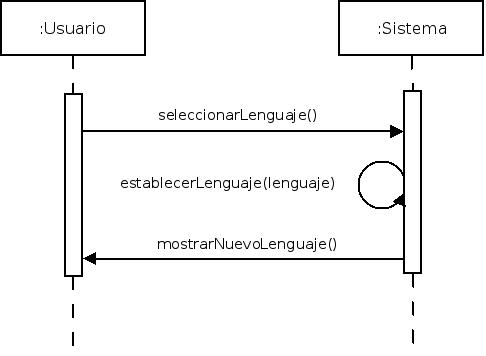
\includegraphics[scale=.55]{img/secuencias/seleccionar-idioma.jpeg}
  \caption{Diagrama de secuencia: Seleccionar lenguage}
  \label{fig:secuencia-seleccionar-lenguaje}
\end{figure}


\textbf{Contrato de operación: seleccionarLenguaje()}
\begin{itemize}
\item \textbf{Referencias cruzadas:} UC-01 (Cuadro \ref{tab:CU-idioma}).
\item \textbf{Responsabilidades:} Seleccionar un nuevo lenguaje a establecer.
\item \textbf{Precondiciones:} Ninguna
\item \textbf{Postcondiciones:}
 \begin{itemize}
\item Se selecciona un nuevo lenguaje, que el sistema utilizará para la interfaz del programa.
\end {itemize}
\end {itemize}

\textbf{Contrato de operación: establecerLenguaje(lenguaje)}
\begin{itemize}
\item \textbf{Referencias cruzadas:} UC-01 (Cuadro \ref{tab:CU-idioma}).
\item \textbf{Responsabilidades:} Establecer un nuevo lenguaje para mostrar la interfaz. Si el usuario está registrado, se establecerá como su lenguaje por defecto.
\item \textbf{Precondiciones:} 
 \begin{itemize}
\item Se ha seleccionado un lenguaje.
\end {itemize}
\item \textbf{Postcondiciones:} 
 \begin{itemize}
\item Establecer el lenguaje recibido como lenguaje para la interfaz.
\item Establecer el lenguaje por defecto para el usuario en caso de haberse identificado.
\end {itemize}
\end {itemize}


\textbf{Contrato de operación: mostrarNuevoLenguaje()}
\begin{itemize}
\item \textbf{Referencias cruzadas:} UC-01 (Cuadro \ref{tab:CU-idioma}).
\item \textbf{Responsabilidades:} Mostrar la interfaz con el nuevo lenguaje establecido.
\item \textbf{Precondiciones:} 
 \begin{itemize}
\item Se ha seleccionado y establecido un lenguaje.
\end {itemize}
\item \textbf{Postcondiciones:} 
 \begin{itemize}
\item La interfaz se muestra en el idioma seleccionado.
\end {itemize}
\end {itemize}

\vspace{10mm}

\begin{figure}[H]
\centering
  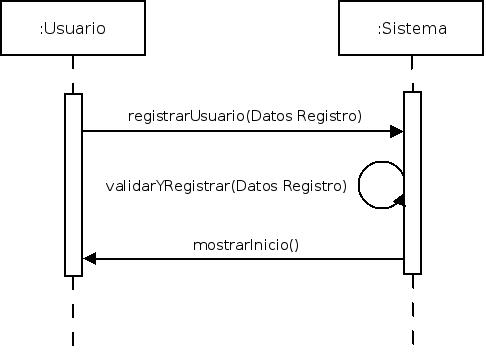
\includegraphics[scale=.55]{img/secuencias/gestion-usuarios-registro.jpeg}
  \caption{Diagrama de secuencia: Gestión de usuarios: Registro de nuevo usuario}
  \label{fig:secuencia-gestion-usuarios-registro}
\end{figure}


\textbf{Contrato de operación: registrarUsuario(Datos Registro)}
\begin{itemize}
\item \textbf{Referencias cruzadas:} UC-02 (Cuadro \ref{tab:CU-registro}).
\item \textbf{Responsabilidades:} Se mandarán los datos de registro de un nuevo usuario al sistema.
\item \textbf{Precondiciones:} Ninguna.
\item \textbf{Postcondiciones:} 
 \begin{itemize}
\item Se mandan los datos pedidos para registrar a un nuevo usuario al sistema.
\end {itemize}
\end {itemize}


\textbf{Contrato de operación: validarYRegistrar(Datos Registro)}
\begin{itemize}
\item \textbf{Referencias cruzadas:} UC-02 (Cuadro \ref{tab:CU-registro}).
\item \textbf{Responsabilidades:} Se validarán los datos recibidos y se realizará el registro del nuevo cliente.
\item \textbf{Precondiciones:} 
 \begin{itemize}
\item El usuario ha de haber enviado el formulario de registro con sus datos.
\end {itemize}
\item \textbf{Postcondiciones:} 
 \begin{itemize}
\item Se valida que los datos recibidos incluyen, al menos, todos los obligatorios.
\item Validación del email a registrar. No puede coincidir con el de algún usuario existente.
\item Registro de un nuevo usuario en el sistema.
\item Se realizará un inicio de sesión del nuevo usuario.
\end {itemize}
\end {itemize}

\textbf{Contrato de operación: mostrarInicio()}
\begin{itemize}
\item \textbf{Referencias cruzadas:} UC-02 (Cuadro \ref{tab:CU-registro}).
\item \textbf{Responsabilidades:} Se navegará hasta la página de inicio de la aplicación web.
\item \textbf{Precondiciones:} 
 \begin{itemize}
\item El usuario ha sido registrado correctamente.
\item El sistema ha iniciado sesión con los datos del usuario.
\end {itemize}
\item \textbf{Postcondiciones:} 
 \begin{itemize}
\item Se muestra la pantalla de inicio del sistema, con los datos del usuario.
\end {itemize}
\end {itemize}

\vspace{10mm}

\begin{figure}[H]
\centering
  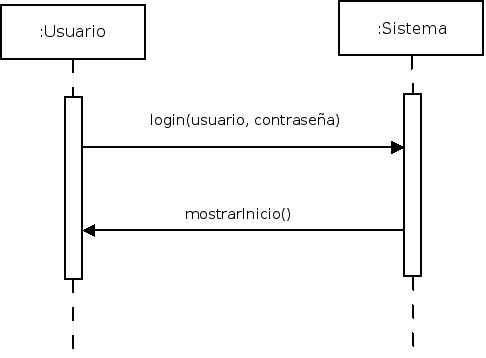
\includegraphics[scale=.55]{img/secuencias/gestion-usuarios-login.jpeg}
  \caption{Diagrama de secuencia: Iniciar sesión}
  \label{fig:secuencia-gestion-usuarios-login}
\end{figure}


\textbf{Contrato de operación: login(usuario, contraseña)}
\begin{itemize}
\item \textbf{Referencias cruzadas:} UC-03 (Cuadro \ref{tab:CU-login}).
\item \textbf{Responsabilidades:} Realizar el login del usuario en el sistema.
\item \textbf{Precondiciones:} 
 \begin{itemize}
\item El usuario no ha iniciado sesión previamente.
\end {itemize}
\item \textbf{Postcondiciones:} 
 \begin{itemize}
\item El sistema habrá comprobado que los datos de accesos son correctos.
\item Se realiza el inicio de la sesión del usuario, quedando este identificado.
\end {itemize}
\end {itemize}

\textbf{Contrato de operación: mostrarInicio()}
\begin{itemize}
\item \textbf{Referencias cruzadas:} UC-03 (Cuadro \ref{tab:CU-login}).
\item \textbf{Responsabilidades:} Se navegará hasta la página de inicio de la aplicación web.
\item \textbf{Precondiciones:} 
 \begin{itemize}
\item El usuario ha sido registrado correctamente.
\item El sistema ha iniciado sesión con los datos del usuario.
\end {itemize}
\item \textbf{Postcondiciones:} 
 \begin{itemize}
\item Se muestra la pantalla de inicio del sistema, con los datos del usuario.
\end {itemize}
\end {itemize}


\vspace{10mm}

\begin{figure}[H]
\centering
  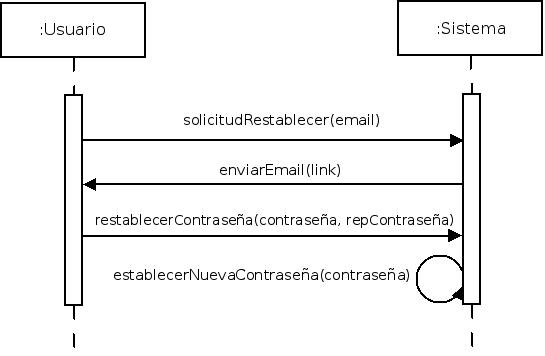
\includegraphics[scale=.55]{img/secuencias/gestion-usuarios-restablecer-contrasena.jpeg}
  \caption{Diagrama de secuencia: Restablecer contraseña}
  \label{fig:secuencia-gestion-usuarios-restablecer-contrasena}
\end{figure}


\textbf{Contrato de operación: solicitudRestablecer(email)}
\begin{itemize}
\item \textbf{Referencias cruzadas:} UC-05 (Cuadro \ref{tab:CU-restablecer-contrasena}).
\item \textbf{Responsabilidades:} Se solicitará al sistema restablecer la contraseña de un usuario que no ha iniciado sesión.
\item \textbf{Precondiciones:} 
 \begin{itemize}
\item El usuario no ha iniciado sesión previamente.
\end {itemize}
\item \textbf{Postcondiciones:} 
 \begin{itemize}
\item Se manda una solicitud de restablecer contraseña al sistema.
\end {itemize}
\end {itemize}

\textbf{Contrato de operación: enviarEmail(link)}
\begin{itemize}
\item \textbf{Referencias cruzadas:} UC-05 (Cuadro \ref{tab:CU-restablecer-contrasena}).
\item \textbf{Responsabilidades:} Se enviará un email al usuario con el enlace para establecer una nueva contraseña.
\item \textbf{Precondiciones:} 
 \begin{itemize}
\item El usuario debe estar registrado en el sistema.
\end {itemize}
\item \textbf{Postcondiciones:} 
 \begin{itemize}
\item Se comprobará que el email pertenece a un usuario registrado.
\item Se envía un email a su correo con el enlace correspondiente para establecer la nueva contraseña.
\end {itemize}
\end {itemize}

\textbf{Contrato de operación: restablecerContraseña(contraseña, repContraseña)}
\begin{itemize}
\item \textbf{Referencias cruzadas:} UC-05 (Cuadro \ref{tab:CU-restablecer-contrasena}).
\item \textbf{Responsabilidades:} Se mandará al sistema una nueva contraseña para el usuario.
\item \textbf{Precondiciones:} Ninguna.
\item \textbf{Postcondiciones:} 
 \begin{itemize}
\item El sistema comprobará que las contraseñas introducidas coinciden.
\end {itemize}
\end {itemize}

\textbf{Contrato de operación: establecerNuevaContraseña(contraseña)}
\begin{itemize}
\item \textbf{Referencias cruzadas:} UC-05 (Cuadro \ref{tab:CU-restablecer-contrasena}).
\item \textbf{Responsabilidades:} Se establecerá una nueva contraseña para el usuario.
\item \textbf{Precondiciones:} 
 \begin{itemize}
\item Se ha introducido la contraseña a establecer como nueva.
\end {itemize}
\item \textbf{Postcondiciones:} 
 \begin{itemize}
\item Se establece la contraseña introducida en la cuenta del usuario.
\item Se inicia sesión con los datos del usuario. 
\end {itemize}
\end {itemize}


\vspace{10mm}

\begin{figure}[H]
\centering
  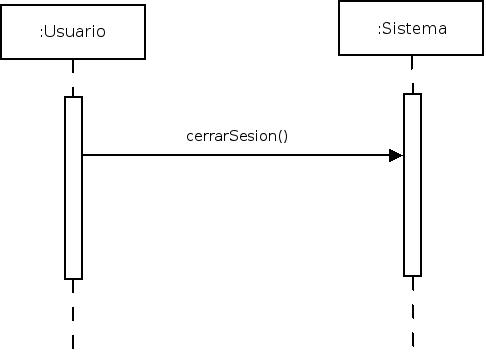
\includegraphics[scale=.55]{img/secuencias/gestion-usuarios-cerrar-sesion.jpeg}
  \caption{Diagrama de secuencia: Cerrar sesión}
  \label{fig:secuencia-gestion-usuarios-cerrar-sesion}
\end{figure}

\textbf{Contrato de operación: cerrarSesion()}
\begin{itemize}
\item \textbf{Referencias cruzadas:} UC-04 (Cuadro \ref{tab:CU-cerrar-sesion}).
\item \textbf{Responsabilidades:} Se cerrará sesión del usuario actualmente identificado.
\item \textbf{Precondiciones:} 
 \begin{itemize}
\item El usuario se ha identificado en el sistema previamente.
\end {itemize}
\item \textbf{Postcondiciones:} 
 \begin{itemize}
\item El sistema terminará la sesión del usuario.
\item La vista actual será redirigida a la página de login.
\end {itemize}
\end {itemize}


\vspace{10mm}

\begin{figure}[H]
\centering
  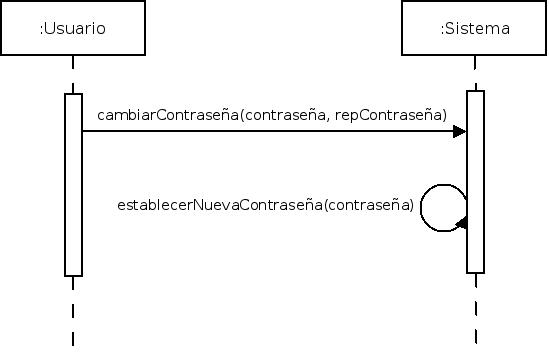
\includegraphics[scale=.55]{img/secuencias/gestion-usuarios-cambiar-contrasena.jpeg}
  \caption{Diagrama de secuencia: Cambiar contraseña}
  \label{fig:secuencia-gestion-usuarios-cambiar-contrasena}
\end{figure}

\textbf{Contrato de operación: cambiarContraseña(contraseña, repContraseña)}
\begin{itemize}
\item \textbf{Referencias cruzadas:} UC-06 (Cuadro \ref{tab:CU-cambiar-contrasena}).
\item \textbf{Responsabilidades:} Se mandará al sistema una nueva contraseña para el usuario.
\item \textbf{Precondiciones:} 
 \begin{itemize}
\item El usuario se ha identificado en el sistema previamente.
\end {itemize}
\item \textbf{Postcondiciones:} 
 \begin{itemize}
\item El sistema comprobará que las contraseñas introducidas coinciden.
\end {itemize}
\end {itemize}

\textbf{Contrato de operación: establecerNuevaContraseña(contraseña)}
\begin{itemize}
\item \textbf{Referencias cruzadas:} UC-06 (Cuadro \ref{tab:CU-cambiar-contrasena}).
\item \textbf{Responsabilidades:} Se establecerá una nueva contraseña para el usuario.
\item \textbf{Precondiciones:} 
 \begin{itemize}
\item Se ha introducido la contraseña a establecer como nueva.
\end {itemize}
\item \textbf{Postcondiciones:} 
 \begin{itemize}
\item Se establece la contraseña introducida en la cuenta del usuario.
\end {itemize}
\end {itemize}


\vspace{10mm}

\begin{figure}[H]
\centering
  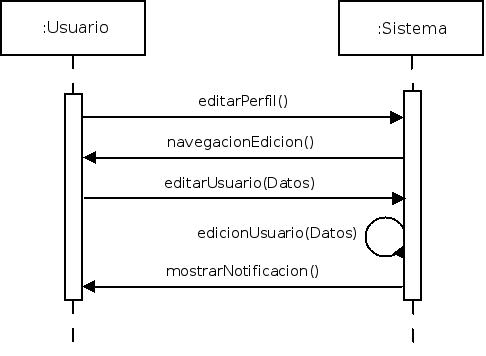
\includegraphics[scale=.55]{img/secuencias/gestion-usuarios-editar-perfil.jpeg}
  \caption{Diagrama de secuencia: Gestión de usuarios: Editar perfil}
  \label{fig:secuencia-gestion-usuarios-editar-perfil}
\end{figure}

\textbf{Contrato de operación: editarPerfil()}
\begin{itemize}
\item \textbf{Referencias cruzadas:} UC-07 (Cuadro \ref{tab:CU-editar-perfil}).
\item \textbf{Responsabilidades:} El usuario enviará al sistema la opción de editar su perfil.
\item \textbf{Precondiciones:} 
 \begin{itemize}
\item El usuario se ha identificado en el sistema previamente.
\item El usuario ha navegado hasta la pantalla de su perfil.
\end {itemize}
\item \textbf{Postcondiciones:} 
 \begin{itemize}
\item Se manda la solicitud de edición del perfil.
\end {itemize}
\end {itemize}

\textbf{Contrato de operación: navegacionEdicion()}
\begin{itemize}
\item \textbf{Referencias cruzadas:} UC-07 (Cuadro \ref{tab:CU-editar-perfil}).
\item \textbf{Responsabilidades:} El sistema mostrará la página correspondiente a la edición de los datos del perfil del usuario.
\item \textbf{Precondiciones:} 
 \begin{itemize}
\item Se ha realizado la acción correspondiente para activar la navegación.
\end {itemize}
\item \textbf{Postcondiciones:} 
 \begin{itemize}
\item Se mostrará la página de edición del perfil del usuario.
\end {itemize}
\end {itemize}

\textbf{Contrato de operación: editarUsuario(Datos)}
\begin{itemize}
\item \textbf{Referencias cruzadas:} UC-07 (Cuadro \ref{tab:CU-editar-perfil}).
\item \textbf{Responsabilidades:} Se mandará al sistema los datos del usuario para que este sea editado.
\item \textbf{Precondiciones:} 
 \begin{itemize}
\item El usuario se ha identificado en el sistema previamente.
\end {itemize}
\item \textbf{Postcondiciones:} 
 \begin{itemize}
\item Se envía el formulario de datos del perfil al sistema.
\end {itemize}
\end {itemize}

\textbf{Contrato de operación: edicionUsuario(Datos)}
\begin{itemize}
\item \textbf{Referencias cruzadas:} UC-07 (Cuadro \ref{tab:CU-editar-perfil}).
\item \textbf{Responsabilidades:} Se realizará la edición de los datos del usuario, guardándolos en el sistema.
\item \textbf{Precondiciones:} 
 \begin{itemize}
\item Se ha enviado el formulario con los datos a editar.
\end {itemize}
\item \textbf{Postcondiciones:} 
 \begin{itemize}
\item El sistema guarda los datos recibidos del usuario en la base de datos.
\end {itemize}
\end {itemize}

\textbf{Contrato de operación: mostrarNotificacion()}
\begin{itemize}
\item \textbf{Referencias cruzadas:} UC-07 (Cuadro \ref{tab:CU-editar-perfil}).
\item \textbf{Responsabilidades:} Se mostrará un mensaje de acción por pantalla.
\item \textbf{Precondiciones:} 
 \begin{itemize}
\item Se ha realizado la acción correspondiente para activar el mensaje.
\end {itemize}
\item \textbf{Postcondiciones:} 
 \begin{itemize}
\item Se muestra el mensaje correspondiente a la acción en la pantalla, a modo de notificación para el usuario. Este puede ser confirmación de la acción o algún tipo de error en la ejecución de la misma.
\end {itemize}
\end {itemize}


\vspace{10mm}

\begin{figure}[H]
\centering
  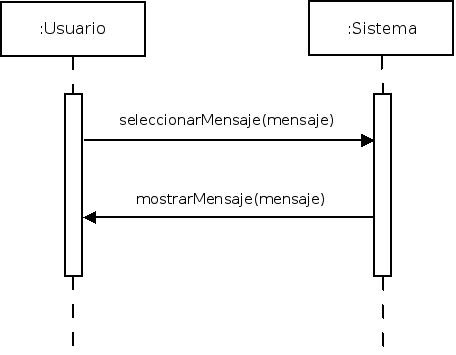
\includegraphics[scale=.55]{img/secuencias/gestion-servicios-leer-correo.jpeg}
  \caption{Diagrama de secuencia: Leer correo interno}
  \label{fig:secuencia-gestion-servicios-leer-correo}
\end{figure}

\textbf{Contrato de operación: seleccionarMensaje(mensaje)}
\begin{itemize}
\item \textbf{Referencias cruzadas:} UC-08 (Cuadro \ref{tab:CU-leer-correo}).
\item \textbf{Responsabilidades:} Se seleccionará el mensaje a mostrar.
\item \textbf{Precondiciones:} 
 \begin{itemize}
\item El usuario se ha identificado en el sistema previamente.
\end {itemize}
\item \textbf{Postcondiciones:} 
 \begin{itemize}
\item El sistema recibirá el mensaje concreto a mostrar.
\end {itemize}
\end {itemize}

\textbf{Contrato de operación: mostrarMensaje(mensaje)}
\begin{itemize}
\item \textbf{Referencias cruzadas:} UC-08 (Cuadro \ref{tab:CU-leer-correo}).
\item \textbf{Responsabilidades:} Se mostrará el mensaje seleccionado al usuario.
\item \textbf{Precondiciones:} 
 \begin{itemize}
\item El mensaje habrá sido seleccionado por el usuario previamente.
\end {itemize}
\item \textbf{Postcondiciones:} 
 \begin{itemize}
\item El sistema muestra la página de visualización de mensajes con los datos detallados del mismo.
\end {itemize}
\end {itemize}


\vspace{10mm}

\begin{figure}[H]
\centering
  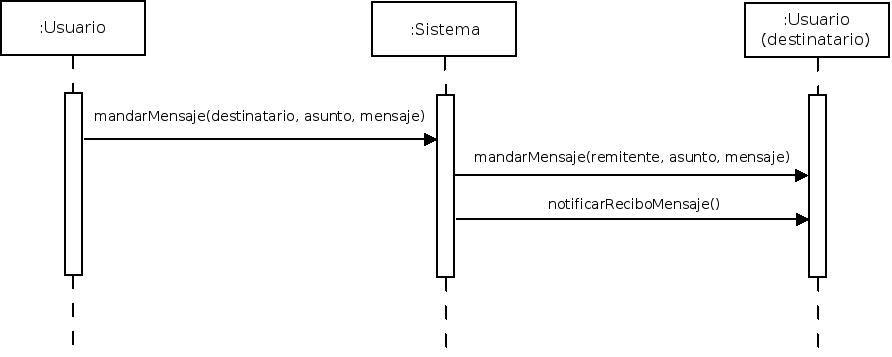
\includegraphics[scale=.45]{img/secuencias/gestion-servicios-mandar-correo.jpeg}
  \caption{Diagrama de secuencia: Mandar correo interno}
  \label{fig:secuencia-gestion-servicios-mandar-correo}
\end{figure}

\textbf{Contrato de operación: mandarMensaje(destinatario, asunto, mensaje)}
\begin{itemize}
\item \textbf{Referencias cruzadas:} UC-09 (Cuadro \ref{tab:CU-mandar-correo}).
\item \textbf{Responsabilidades:} Se mandará al sistema el mensaje que se desea enviar, junto al asunto y el destinatario.
\item \textbf{Precondiciones:} 
 \begin{itemize}
\item El usuario se ha identificado en el sistema previamente.
\end {itemize}
\item \textbf{Postcondiciones:} 
 \begin{itemize}
\item El sistema recibirá los datos del mensaje: El cuerpo (mensaje en sí), asunto y destinatario).
\end {itemize}
\end {itemize}

\textbf{Contrato de operación: mandarMensaje(remitente, asunto, mensaje)}
\begin{itemize}
\item \textbf{Referencias cruzadas:} UC-09 (Cuadro \ref{tab:CU-mandar-correo}).
\item \textbf{Responsabilidades:} El sistema mandará el mensaje recibido a su destinatario.
\item \textbf{Precondiciones:} 
 \begin{itemize}
\item Se ha recibido el mensaje por parte del remitente.
\end {itemize}
\item \textbf{Postcondiciones:} 
 \begin{itemize}
\item El sistema manda al destinatario el mensaje recibido.
\end {itemize}
\end {itemize}

\textbf{Contrato de operación: notificarReciboMensaje()}
\begin{itemize}
\item \textbf{Referencias cruzadas:} UC-09 (Cuadro \ref{tab:CU-mandar-correo}).
\item \textbf{Responsabilidades:} Notificar al destinatario del mensaje que ha recibido un correo interno.
\item \textbf{Precondiciones:} 
 \begin{itemize}
\item El usuario ha mandado un correo al usuario.
\end {itemize}
\item \textbf{Postcondiciones:} 
 \begin{itemize}
\item Se creará una nueva notificación de recibo de mensaje para el destinatario.
\end {itemize}
\end {itemize}


\vspace{10mm}

\begin{figure}[H]
\centering
  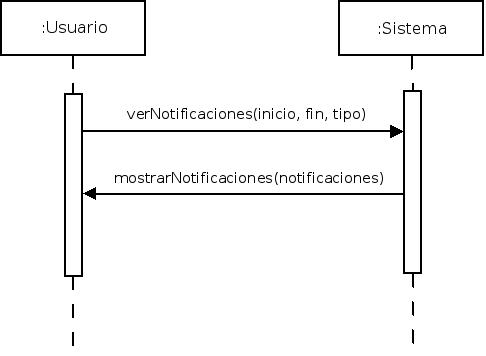
\includegraphics[scale=.50]{img/secuencias/notificaciones.jpeg}
  \caption{Diagrama de secuencia: Notificaciones}
  \label{fig:secuencia-notificaciones}
\end{figure}

\textbf{Contrato de operación: verNotificaciones(inicio, fin, tipo)}
\begin{itemize}
\item \textbf{Referencias cruzadas:} UC-10 (Cuadro \ref{tab:CU-notificaciones}).
\item \textbf{Responsabilidades:} Solicitar las notificaciones destinadas al usuario en unas determinadas fechas.
\item \textbf{Precondiciones:} 
 \begin{itemize}
\item El usuario se ha identificado en el sistema previamente.
\end {itemize}
\item \textbf{Postcondiciones:} 
 \begin{itemize}
\item Se envía al sistema el formulario con las fechas de inicio y fin elegidas para ver las notificaciones del usuario en el sistema. Se podrá mandar el tipo de notificación específica a mostrar.
\end {itemize}
\end {itemize}

\textbf{Contrato de operación: mostrarNotificaciones(notificaciones)}
\begin{itemize}
\item \textbf{Referencias cruzadas:} UC-10 (Cuadro \ref{tab:CU-notificaciones}).
\item \textbf{Responsabilidades:} Mostrar las notificaciones destinadas al usuario.
\item \textbf{Precondiciones:} 
 \begin{itemize}
\item El usuario ha solicitado ver sus notificaciones.
\end {itemize}
\item \textbf{Postcondiciones:} 
 \begin{itemize}
\item Se muestra el listado de notificaciones para el usuario entre las fechas seleccionadas.
\end {itemize}
\end {itemize}


\vspace{10mm}

\begin{figure}[H]
\centering
  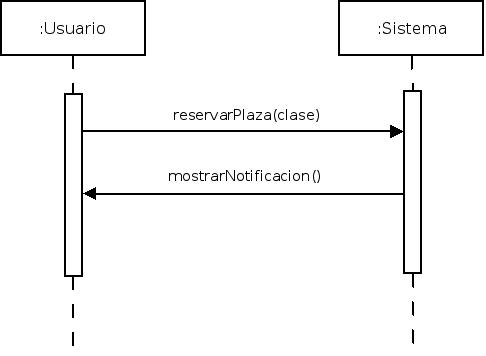
\includegraphics[scale=.55]{img/secuencias/gestion-servicios-reservar-clase.jpeg}
  \caption{Diagrama de secuencia: Gestión de servicios: Reservar plaza en una clase}
  \label{fig:secuencia-gestion-servicios-reservar-clase}
\end{figure}

\textbf{Contrato de operación: reservarPlaza(clase)}
\begin{itemize}
\item \textbf{Referencias cruzadas:} UC-11 (Cuadro \ref{tab:CU-reservar-clase}).
\item \textbf{Responsabilidades:} Se reservará una plaza de la clase seleccionada al usuario.
\item \textbf{Precondiciones:} 
 \begin{itemize}
\item El usuario se ha identificado en el sistema previamente.
\item Ha de haber al menos una plaza libre en la clase.
\item El usuario no posee plaza en la clase seleccionada.
\end {itemize}
\item \textbf{Postcondiciones:} 
 \begin{itemize}
\item Se reservará una plaza de la clase seleccionada al usuario.
\item Se reduce la plaza reservada de las totales disponibles de la clase.
\end {itemize}
\end {itemize}

\textbf{Contrato de operación: mostrarNotificacion()}
\begin{itemize}
\item \textbf{Referencias cruzadas:} UC-11 (Cuadro \ref{tab:CU-reservar-clase}).
\item \textbf{Responsabilidades:} Se mostrará un mensaje de acción por pantalla.
\item \textbf{Precondiciones:} 
 \begin{itemize}
\item Se ha realizado la acción correspondiente para activar el mensaje.
\end {itemize}
\item \textbf{Postcondiciones:} 
 \begin{itemize}
\item Se muestra el mensaje correspondiente a la acción en la pantalla, a modo de notificación para el usuario. Este puede ser confirmación de la acción o algún tipo de error en la ejecución de la misma.
\end {itemize}
\end {itemize}


\vspace{10mm}

\begin{figure}[H]
\centering
  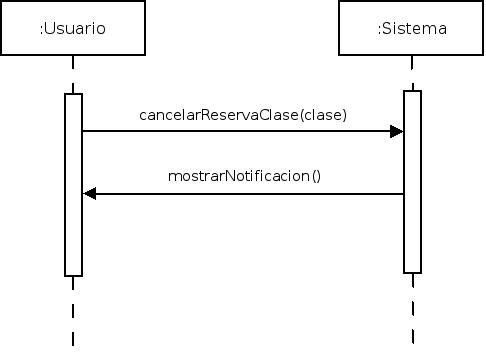
\includegraphics[scale=.55]{img/secuencias/gestion-servicios-cancelar-reserva-clase.jpeg}
  \caption{Diagrama de secuencia: Gestión de servicios: Cancelación de reserva de una clase}
  \label{fig:secuencia-gestion-servicios-cancelar-reserva-clase}
\end{figure}

\textbf{Contrato de operación: cancelarReservaClase(clase)}
\begin{itemize}
\item \textbf{Referencias cruzadas:} UC-12 (Cuadro \ref{tab:CU-cancelar-reserva-clase}).
\item \textbf{Responsabilidades:} Se cancelará la reserva del usuario previamente realizada de una clase específica.
\item \textbf{Precondiciones:} 
 \begin{itemize}
\item El usuario se ha identificado en el sistema previamente.
\item La clase ha sido reservada previamente.
\end {itemize}
\item \textbf{Postcondiciones:} 
 \begin{itemize}
\item Se cancela la reserva de la plaza del usuario en la clase específica.
\item Las plazas disponibles de la clase en concreto se incrementan en uno.
\end {itemize}
\end {itemize}

\textbf{Contrato de operación: mostrarNotificacion()}
\begin{itemize}
\item \textbf{Referencias cruzadas:} UC-12 (Cuadro \ref{tab:CU-cancelar-reserva-clase}).
\item \textbf{Responsabilidades:} Se mostrará un mensaje de acción por pantalla.
\item \textbf{Precondiciones:} 
 \begin{itemize}
\item Se ha realizado la acción correspondiente para activar el mensaje.
\end {itemize}
\item \textbf{Postcondiciones:} 
 \begin{itemize}
\item Se muestra el mensaje correspondiente a la acción en la pantalla, a modo de notificación para el usuario. Este puede ser confirmación de la acción o algún tipo de error en la ejecución de la misma.
\end {itemize}
\end {itemize}


\vspace{10mm}

\begin{figure}[H]
\centering
  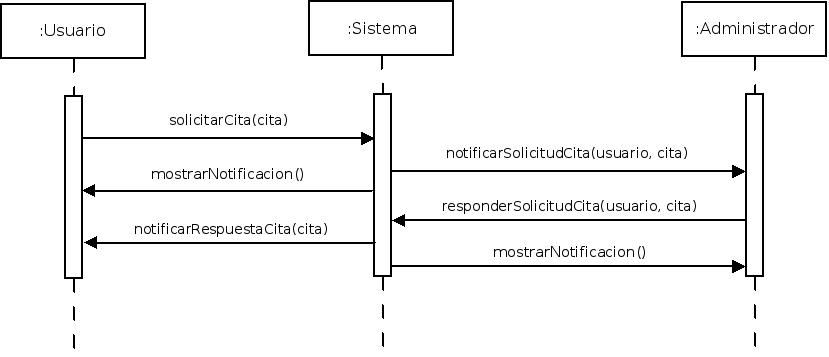
\includegraphics[scale=.45]{img/secuencias/gestion-servicios-solicitar-responder-cita.jpeg}
  \caption{Diagrama de secuencia:: Gestión de servicios: Solicitud de cita y respuesta}
  \label{fig:secuencia-gestion-servicios-solicitar-responder-cita.jpeg}
\end{figure}

\textbf{Contrato de operación: solicitarCita(cita)}
\begin{itemize}
\item \textbf{Referencias cruzadas:} UC-13 (Cuadro \ref{tab:CU-solicitar-cita}), UC-14 (Cuadro \ref{tab:CU-responder-solicitud-cita}).
\item \textbf{Responsabilidades:} Se enviará una solicitud de la cita seleccionada a los administradores.
\item \textbf{Precondiciones:} 
 \begin{itemize}
\item El usuario se ha identificado en el sistema previamente.
\item La cita debe estar disponible para su solicitud.
\end {itemize}
\item \textbf{Postcondiciones:} 
 \begin{itemize}
\item Se enviará una solicitud de la cita seleccionada a los administradores.
\item Se establece la cita como no disponible hasta que se resuelva la solicitud.
\end {itemize}
\end {itemize}

\textbf{Contrato de operación: notificarSolicitudCita(usuario, cita)}
\begin{itemize}
\item \textbf{Referencias cruzadas:} UC-13 (Cuadro \ref{tab:CU-solicitar-cita}), UC-14 (Cuadro \ref{tab:CU-responder-solicitud-cita}).
\item \textbf{Responsabilidades:} Mandar una notificación de solicitud de cita de un determinado usuario a los administradores.
\item \textbf{Precondiciones:} 
 \begin{itemize}
\item Se ha recibido una solicitud de cita en el sistema.
\end {itemize}
\item \textbf{Postcondiciones:} 
 \begin{itemize}
\item Se creará una nueva notificación de solicitud de cita para los administradores.
\end {itemize}
\end {itemize}

\textbf{Contrato de operación: mostrarNotificacion()}
\begin{itemize}
\item \textbf{Referencias cruzadas:} UC-13 (Cuadro \ref{tab:CU-solicitar-cita}), UC-14 (Cuadro \ref{tab:CU-responder-solicitud-cita}).
\item \textbf{Responsabilidades:} Se mostrará un mensaje de acción por pantalla.
\item \textbf{Precondiciones:} 
 \begin{itemize}
\item Se ha realizado la acción correspondiente para activar el mensaje.
\end {itemize}
\item \textbf{Postcondiciones:} 
 \begin{itemize}
\item Se muestra el mensaje correspondiente a la acción en la pantalla, a modo de notificación para el usuario. Este puede ser confirmación de la acción o algún tipo de error en la ejecución de la misma.
\end {itemize}
\end {itemize}

\textbf{Contrato de operación: responderSolicitudCita(usuario, cita)}
\begin{itemize}
\item \textbf{Referencias cruzadas:} UC-13 (Cuadro \ref{tab:CU-solicitar-cita}), UC-14 (Cuadro \ref{tab:CU-responder-solicitud-cita}).
\item \textbf{Responsabilidades:} Responder a la solicitud de cita recibida por parte de un usuario específico.
\item \textbf{Precondiciones:} 
 \begin{itemize}
\item El administrador se ha identificado en el sistema previamente.
\item Se ha recibido una solicitud de cita por parte de un determinado usuario.
\end {itemize}
\item \textbf{Postcondiciones:} 
 \begin{itemize}
\item Se envía la respuesta de la solicitud al sistema.
\item Dependiendo de la respuesta (declinada o aceptada), se establece la disponibilidad de la cita (disponible o no disponible).
\end {itemize}
\end {itemize}

\textbf{Contrato de operación: notificarRespuestaCita(cita)}
\begin{itemize}
\item \textbf{Referencias cruzadas:} UC-13 (Cuadro \ref{tab:CU-solicitar-cita}), UC-14 (Cuadro \ref{tab:CU-responder-solicitud-cita}).
\item \textbf{Responsabilidades:} Mandar una notificación de respuesta de la solicitud de cita al usuario.
\item \textbf{Precondiciones:} 
 \begin{itemize}
\item Se ha recibido una respuesta de la solicitud de cita por parte de los administradores.
\end {itemize}
\item \textbf{Postcondiciones:} 
 \begin{itemize}
\item Se creará una nueva notificación de repuesta de solicitud de cita para el usuario.
\end {itemize}
\end {itemize}


\vspace{10mm}

\begin{figure}[H]
\centering
  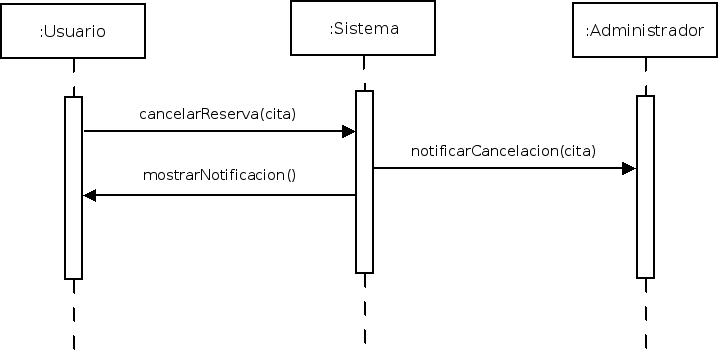
\includegraphics[scale=.50]{img/secuencias/gestion-servicios-cancelar-cita-por-parte-de-usuario.jpeg}
  \caption{Diagrama de secuencia: Gestión de servicios: Cancelar Cita}
  \label{fig:secuencia-gestion-servicios-cancelar-cita-por-parte-de-usuario}
\end{figure}

\textbf{Contrato de operación: cancelarReserva(cita)}
\begin{itemize}
\item \textbf{Referencias cruzadas:} UC-15 (Cuadro \ref{tab:CU-cancelar-cita}).
\item \textbf{Responsabilidades:} Se cancelará la cita o solicitud de cita del usuario, notificando a los administradores.
\item \textbf{Precondiciones:} 
 \begin{itemize}
\item El usuario se ha identificado en el sistema previamente.
\item El usuario ha solicitado la cita.
\end {itemize}
\item \textbf{Postcondiciones:} 
 \begin{itemize}
\item Se cancela la reserva o solicitud de la cita seleccionada.
\end {itemize}
\end {itemize}

\textbf{Contrato de operación: notificarCancelacion(cita)}
\begin{itemize}
\item \textbf{Referencias cruzadas:} UC-15 (Cuadro \ref{tab:CU-cancelar-cita}).
\item \textbf{Responsabilidades:} Mandar una notificación de cancelación de la reserva o solicitud de cita a los administradores.
\item \textbf{Precondiciones:} 
 \begin{itemize}
\item Se ha cancelado una solicitud o reserva de cita.
\end {itemize}
\item \textbf{Postcondiciones:} 
 \begin{itemize}
\item Se creará una nueva notificación de cancelación de reserva o solicitud de cita para los administradores.
\end {itemize}
\end {itemize}

\textbf{Contrato de operación: mostrarNotificacion()}
\begin{itemize}
\item \textbf{Referencias cruzadas:} UC-15 (Cuadro \ref{tab:CU-cancelar-cita}).
\item \textbf{Responsabilidades:} Se mostrará un mensaje de acción por pantalla.
\item \textbf{Precondiciones:} 
 \begin{itemize}
\item Se ha realizado la acción correspondiente para activar el mensaje.
\end {itemize}
\item \textbf{Postcondiciones:} 
 \begin{itemize}
\item Se muestra el mensaje correspondiente a la acción en la pantalla, a modo de notificación para el usuario. Este puede ser confirmación de la acción o algún tipo de error en la ejecución de la misma.
\end {itemize}
\end {itemize}


\vspace{10mm}

\begin{figure}[H]
\centering
  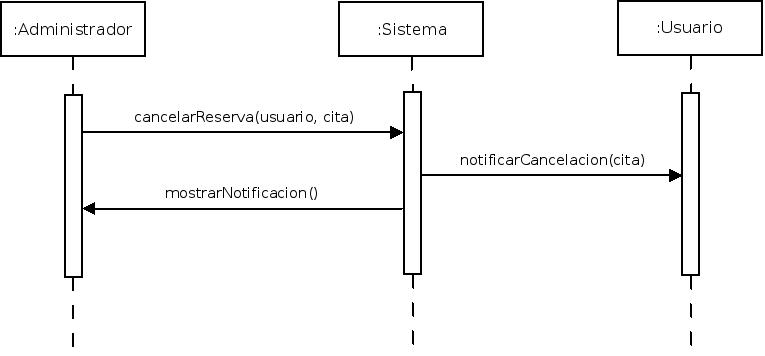
\includegraphics[scale=.50]{img/secuencias/gestion-servicios-cancelar-cita-por-parte-de-admin.jpeg}
  \caption{Diagrama de secuencia: Gestión de servicios: Cancelar cita (Administrador)}
  \label{fig:secuencia-gestion-servicios-cancelar-cita-por-parte-de-admin}
\end{figure}

\textbf{Contrato de operación: cancelarReserva(cita)}
\begin{itemize}
\item \textbf{Referencias cruzadas:} UC-16 (Cuadro \ref{tab:CU-cancelar-cita-admin}).
\item \textbf{Responsabilidades:} Un administrador cancelará la cita o solicitud de cita del usuario, notificando al mismo.
\item \textbf{Precondiciones:} 
 \begin{itemize}
\item El administrador se ha identificado en el sistema previamente.
\item El usuario ha solicitado la cita.
\end {itemize}
\item \textbf{Postcondiciones:} 
 \begin{itemize}
\item Se cancela la reserva o solicitud de la cita seleccionada.
\end {itemize}
\end {itemize}

\textbf{Contrato de operación: notificarCancelacion(cita)}
\begin{itemize}
\item \textbf{Referencias cruzadas:} UC-16 (Cuadro \ref{tab:CU-cancelar-cita-admin}).
\item \textbf{Responsabilidades:} Mandar una notificación de cancelación de la reserva o solicitud de cita al usuario.
\item \textbf{Precondiciones:} 
 \begin{itemize}
\item Se ha cancelado una solicitud o reserva de cita.
\end {itemize}
\item \textbf{Postcondiciones:} 
 \begin{itemize}
\item Se creará una nueva notificación de cancelación de reserva o solicitud de cita para el usuario.
\end {itemize}
\end {itemize}

\textbf{Contrato de operación: mostrarNotificacion()}
\begin{itemize}
\item \textbf{Referencias cruzadas:} UC-16 (Cuadro \ref{tab:CU-cancelar-cita-admin}).
\item \textbf{Responsabilidades:} Se mostrará un mensaje de acción por pantalla.
\item \textbf{Precondiciones:} 
 \begin{itemize}
\item Se ha realizado la acción correspondiente para activar el mensaje.
\end {itemize}
\item \textbf{Postcondiciones:} 
 \begin{itemize}
\item Se muestra el mensaje correspondiente a la acción en la pantalla, a modo de notificación para el administrador. Este puede ser confirmación de la acción o algún tipo de error en la ejecución de la misma.
\end {itemize}
\end {itemize}


\vspace{10mm}

\begin{figure}[H]
\centering
  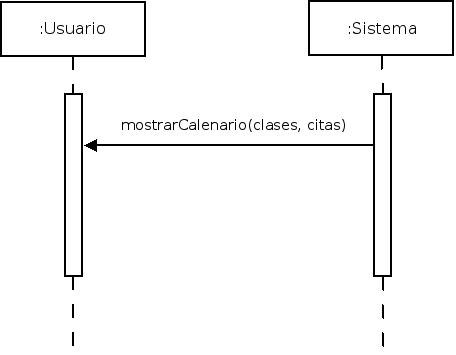
\includegraphics[scale=.55]{img/secuencias/gestion-servicios-calendario.jpeg}
  \caption{Diagrama de secuencia: Gestión de servicios: Calendario de actividades}
  \label{fig:secuencia-gestion-servicios-calendario}
\end{figure}

\textbf{Contrato de operación: mostrarCalendario(clases, citas)}
\begin{itemize}
\item \textbf{Referencias cruzadas:} UC-17 (Cuadro \ref{tab:CU-calendario}).
\item \textbf{Responsabilidades:} Mostrar el calendario mensual con las clases y citas disponibles en el sistema. Se distinguirá el estado de las mismas por su color de fondo o borde, para diferenciar entre clases o citas pasadas, disponibles, reservadas por el usuario...
\item \textbf{Precondiciones:} 
 \begin{itemize}
\item El usuario se ha identificado en el sistema previamente.
\item El usuario ha accedido a la página de visualización del calendario.
\end {itemize}
\item \textbf{Postcondiciones:} 
 \begin{itemize}
\item El sistema muestra el calendario con todas las citas y clases disponibles, distinguiendo su estado por colores. 
\end {itemize}
\end {itemize}


\vspace{10mm}

\begin{figure}[H]
\centering
  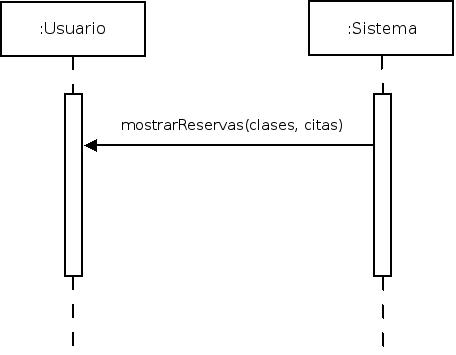
\includegraphics[scale=.55]{img/secuencias/gestion-servicios-reservas.jpeg}
  \caption{Diagrama de secuencia: Gestión de servicios: Consultar reservas}
  \label{fig:secuencia-gestion-servicios-reservas}
\end{figure}

\textbf{Contrato de operación: mostrarReservas(citas, clases)}
\begin{itemize}
\item \textbf{Referencias cruzadas:} UC-18 (Cuadro \ref{tab:CU-reservas}).
\item \textbf{Responsabilidades:} Se mostrará una lista de las citas y reservas del usuario, tanto pasadas como actuales.
\item \textbf{Precondiciones:} 
 \begin{itemize}
\item El usuario se ha identificado en el sistema previamente.
\item El usuario ha navegado hasta la página de vista de reservas.
\end {itemize}
\item \textbf{Postcondiciones:} 
 \begin{itemize}
\item Se listarán todas las citas y clases que el usuario haya reservado, distinguiendo entre pasadas y actuales.
\end {itemize}
\end {itemize}


\vspace{10mm}

\begin{figure}[H]
\centering
  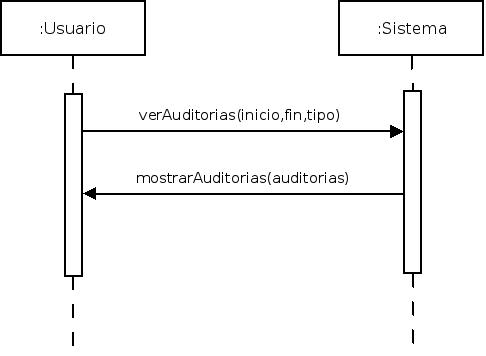
\includegraphics[scale=.55]{img/secuencias/auditorias.jpeg}
  \caption{Diagrama de secuencia: Auditorías}
  \label{fig:secuencia-auditorias}
\end{figure}

\textbf{Contrato de operación: verAuditorias(inicio, fin, tipo)}
\begin{itemize}
\item \textbf{Referencias cruzadas:} UC-19 (Cuadro \ref{tab:CU-auditorias}).
\item \textbf{Responsabilidades:} Solicitar las acciones llevadas a cabo por el usuario en unas determinadas fechas.
\item \textbf{Precondiciones:} 
 \begin{itemize}
\item El usuario se ha identificado en el sistema previamente.
\end {itemize}
\item \textbf{Postcondiciones:} 
 \begin{itemize}
\item Se envía al sistema el formulario con las fechas de inicio y fin elegidas para ver las acciones del usuario en el sistema. Se podrá mandar el tipo de acción específica a mostrar.
\end {itemize}
\end {itemize}

\textbf{Contrato de operación: mostrarAuditorias(auditorias)}
\begin{itemize}
\item \textbf{Referencias cruzadas:} UC-19 (Cuadro \ref{tab:CU-auditorias}).
\item \textbf{Responsabilidades:} Mostrar las acciones llevadas a cabo por el usuario en el sistema.
\item \textbf{Precondiciones:} 
 \begin{itemize}
\item El usuario ha solicitado ver sus auditorías.
\end {itemize}
\item \textbf{Postcondiciones:} 
 \begin{itemize}
\item Se muestra el listado de acciones realizadas entre las fechas seleccionadas.
\end {itemize}
\end {itemize}


\vspace{10mm}

\begin{figure}[H]
\centering
  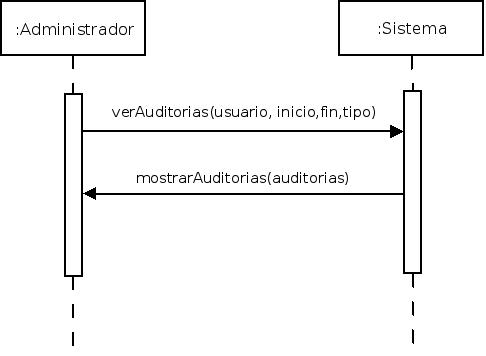
\includegraphics[scale=.55]{img/secuencias/auditorias-administrador.jpeg}
  \caption{Diagrama de secuencia: Auditorías de Administradores}
  \label{fig:secuencia-auditorias-administrador}
\end{figure}

\textbf{Contrato de operación: verAuditorias(usuario, inicio, fin, tipo)}
\begin{itemize}
\item \textbf{Referencias cruzadas:} UC-20 (Cuadro \ref{tab:CU-auditorias-admin}).
\item \textbf{Responsabilidades:} Solicitar las acciones llevadas a cabo por el usuario seleccionado en unas determinadas fechas.
\item \textbf{Precondiciones:} 
 \begin{itemize}
\item El administrador se ha identificado en el sistema previamente.
\end {itemize}
\item \textbf{Postcondiciones:} 
 \begin{itemize}
\item Se envía al sistema el formulario con el usuario específico y las fechas de inicio y fin elegidas para ver las acciones del usuario en el sistema. Se podrá mandar el tipo de acción específica a mostrar.
\end {itemize}
\end {itemize}

\textbf{Contrato de operación: mostrarAuditorias(auditorias)}
\begin{itemize}
\item \textbf{Referencias cruzadas:} UC-20 (Cuadro \ref{tab:CU-auditorias-admin}).
\item \textbf{Responsabilidades:} Mostrar las acciones llevadas a cabo por el usuario seleccionado en el sistema.
\item \textbf{Precondiciones:} 
 \begin{itemize}
\item El administrador ha solicitado ver las auditorías seleccionadas.
\end {itemize}
\item \textbf{Postcondiciones:} 
 \begin{itemize}
\item Se muestra el listado de acciones realizadas entre las fechas seleccionadas para el usuario especificado.
\end {itemize}
\end {itemize}

\vspace{10mm}

\begin{figure}[H]
\centering
  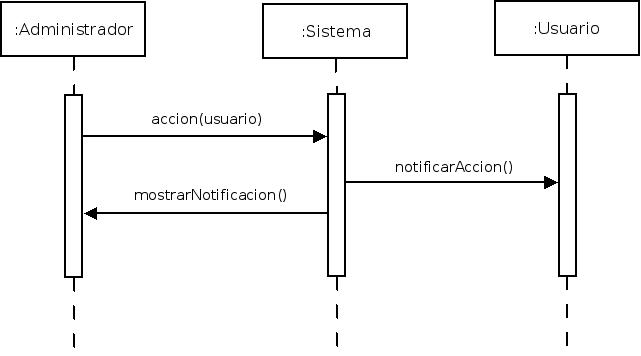
\includegraphics[scale=.50]{img/secuencias/gestion-usuarios-activar-suspender.jpeg}
  \caption{Diagrama de secuencia: Gestión de usuarios: Activar/Suspender}
  \label{fig:secuencia-gestion-usuarios-activar-suspender}
\end{figure}

\textbf{Contrato de operación: accion(usuario)}
\begin{itemize}
\item \textbf{Referencias cruzadas:} UC-21 (Cuadro \ref{tab:CU-activar-suspender-usuario}).
\item \textbf{Responsabilidades:} El administrador podrá activar o suspender al usuario seleccionado.
\item \textbf{Precondiciones:} 
 \begin{itemize}
\item El administrador se ha identificado en el sistema previamente.
\item El usuario seleccionado debe estar activo para ser suspendido o viceversa.
\end {itemize}
\item \textbf{Postcondiciones:} 
 \begin{itemize}
\item Se realizará la acción seleccionada por el administrador \textit{(activar, suspender)} referente a un usuario específico.
\end {itemize}
\end {itemize}

\textbf{Contrato de operación: notificarAccion()}
\begin{itemize}
\item \textbf{Referencias cruzadas:} UC-21 (Cuadro \ref{tab:CU-activar-suspender-usuario}).
\item \textbf{Responsabilidades:} Mandar una notificación de suspensión/activación de la cuenta al usuario.
\item \textbf{Precondiciones:} 
 \begin{itemize}
\item Se ha suspendido/activado la cuenta de un usuario.
\end {itemize}
\item \textbf{Postcondiciones:} 
 \begin{itemize}
\item Se creará una nueva notificación de activación o suspensión de cuenta para el usuario seleccionado.
\end {itemize}
\end {itemize}

\textbf{Contrato de operación: mostrarNotificacion()}
\begin{itemize}
\item \textbf{Referencias cruzadas:} UC-21 (Cuadro \ref{tab:CU-activar-suspender-usuario}).
\item \textbf{Responsabilidades:} Se mostrará un mensaje de acción por pantalla.
\item \textbf{Precondiciones:} 
 \begin{itemize}
\item Se ha realizado la acción correspondiente para activar el mensaje.
\end {itemize}
\item \textbf{Postcondiciones:} 
 \begin{itemize}
\item Se muestra el mensaje correspondiente a la acción en la pantalla, a modo de notificación para el administrador. Este puede ser confirmación de la acción o algún tipo de error en la ejecución de la misma.
\end {itemize}
\end {itemize}


\vspace{10mm}

\begin{figure}[H]
\centering
  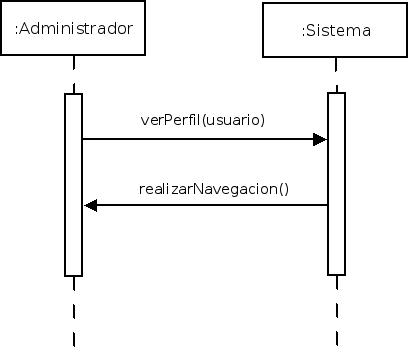
\includegraphics[scale=.55]{img/secuencias/gestion-usuarios-ver-perfil.jpeg}
  \caption{Diagrama de secuencia: Gestión de usuarios: Ver perfil (Administrador)}
  \label{fig:secuencia-gestion-usuarios-ver-perfil}
\end{figure}

\textbf{Contrato de operación: verPerfil(usuario)}
\begin{itemize}
\item \textbf{Referencias cruzadas:} UC-22 (Cuadro \ref{tab:CU-ver-perfil-admin}).
\item \textbf{Responsabilidades:} El administrador podrá ver el perfil del usuario seleccionado.
\item \textbf{Precondiciones:} 
 \begin{itemize}
\item El administrador se ha identificado en el sistema previamente.
\end {itemize}
\item \textbf{Postcondiciones:} 
 \begin{itemize}
\item Se navegará a la página correspondiente para ver los detalles del perfil de un usuario específico.
\end {itemize}
\end {itemize}

\textbf{Contrato de operación: realizarNavegacion()}
\begin{itemize}
\item \textbf{Referencias cruzadas:} UC-22 (Cuadro \ref{tab:CU-ver-perfil-admin}).
\item \textbf{Responsabilidades:} El sistema mostrará la página correspondiente al perfil del usuario.
\item \textbf{Precondiciones:} 
 \begin{itemize}
\item Se ha realizado la acción correspondiente para activar la navegación.
\end {itemize}
\item \textbf{Postcondiciones:} 
 \begin{itemize}
\item Se mostrará la página del perfil de usuario al administrador.
\end {itemize}
\end {itemize}


\vspace{10mm}

\begin{figure}[H]
\centering
  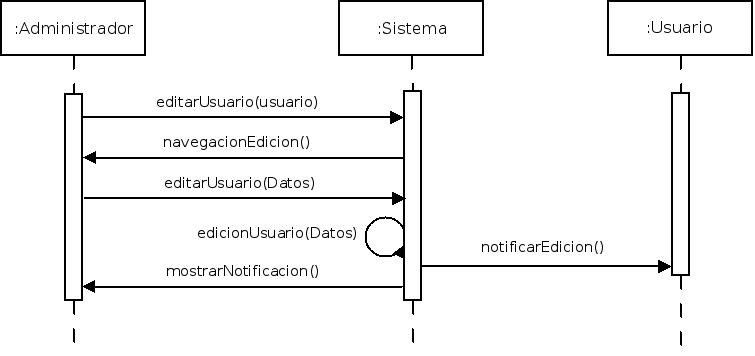
\includegraphics[scale=.50]{img/secuencias/gestion-usuarios-editar-usuario-administrador.jpeg}
  \caption{Diagrama de secuencia: Gestión de usuarios: Editar usuario (Administrador)}
  \label{fig:secuencia-gestion-usuarios-editar-usuario-administrador}
\end{figure}

\textbf{Contrato de operación: editarUsuario(usuario)}
\begin{itemize}
\item \textbf{Referencias cruzadas:} UC-23 (Cuadro \ref{tab:CU-editar-usuario-admin}).
\item \textbf{Responsabilidades:} Se informará al sistema de la acción de edición de un usuario específico.
\item \textbf{Precondiciones:} 
 \begin{itemize}
\item El administrador se ha identificado en el sistema previamente.
\end {itemize}
\item \textbf{Postcondiciones:} 
 \begin{itemize}
\item Se manda la solicitud de edición del usuario seleccionado.
\end {itemize}
\end {itemize}

\textbf{Contrato de operación: navegacionEdicion()}
\begin{itemize}
\item \textbf{Referencias cruzadas:} UC-23 (Cuadro \ref{tab:CU-editar-usuario-admin}).
\item \textbf{Responsabilidades:} El sistema mostrará la página correspondiente a la edición de los datos del usuario.
\item \textbf{Precondiciones:} 
 \begin{itemize}
\item Se ha realizado la acción correspondiente para activar la navegación.
\end {itemize}
\item \textbf{Postcondiciones:} 
 \begin{itemize}
\item Se mostrará la página de edición del perfil del usuario seleccionado.
\end {itemize}
\end {itemize}

\textbf{Contrato de operación: editarUsuario(Datos)}
\begin{itemize}
\item \textbf{Referencias cruzadas:} UC-23 (Cuadro \ref{tab:CU-editar-usuario-admin}).
\item \textbf{Responsabilidades:} Se mandará al sistema los datos del usuario para que este sea editado.
\item \textbf{Precondiciones:} 
 \begin{itemize}
\item El administrador se ha identificado en el sistema previamente.
\end {itemize}
\item \textbf{Postcondiciones:} 
 \begin{itemize}
\item Se envía el formulario de datos del cliente a editar al sistema.
\end {itemize}
\end {itemize}

\textbf{Contrato de operación: edicionUsuario(Datos)}
\begin{itemize}
\item \textbf{Referencias cruzadas:} UC-23 (Cuadro \ref{tab:CU-editar-usuario-admin}).
\item \textbf{Responsabilidades:} Se realizará la edición de los datos del usuario, guardándolos en el sistema.
\item \textbf{Precondiciones:} 
 \begin{itemize}
\item Se ha enviado el formulario con los datos a editar.
\end {itemize}
\item \textbf{Postcondiciones:} 
 \begin{itemize}
\item El sistema guarda los datos recibidos para el usuario específico en la base de datos.
\end {itemize}
\end {itemize}

\textbf{Contrato de operación: notificarEdicion()}
\begin{itemize}
\item \textbf{Referencias cruzadas:} UC-23 (Cuadro \ref{tab:CU-editar-usuario-admin}).
\item \textbf{Responsabilidades:} Mandar una notificación de edición del perfil por parte del administrador al usuario.
\item \textbf{Precondiciones:} 
 \begin{itemize}
\item Se ha editado los datos del usuario por parte del administrador.
\end {itemize}
\item \textbf{Postcondiciones:} 
 \begin{itemize}
\item Se creará una nueva notificación de edición del perfil para el usuario seleccionado, indicando quién lo ha modificado.
\end {itemize}
\end {itemize}

\textbf{Contrato de operación: mostrarNotificacion()}
\begin{itemize}
\item \textbf{Referencias cruzadas:} UC-23 (Cuadro \ref{tab:CU-editar-usuario-admin}).
\item \textbf{Responsabilidades:} Se mostrará un mensaje de acción por pantalla.
\item \textbf{Precondiciones:} 
 \begin{itemize}
\item Se ha realizado la acción correspondiente para activar el mensaje.
\end {itemize}
\item \textbf{Postcondiciones:} 
 \begin{itemize}
\item Se muestra el mensaje correspondiente a la acción en la pantalla, a modo de notificación para el administrador. Este puede ser confirmación de la acción o algún tipo de error en la ejecución de la misma.
\end {itemize}
\end {itemize}


\vspace{10mm}

\begin{figure}[H]
\centering
  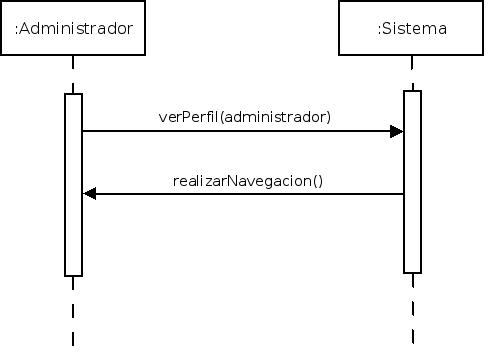
\includegraphics[scale=.55]{img/secuencias/gestion-administradores-ver-perfil.jpeg}
  \caption{Diagrama de secuencia: Gestión de administradores: Ver perfil de administrador}
  \label{fig:secuencia-gestion-administradores-ver-perfil}
\end{figure}

\textbf{Contrato de operación: verPerfil(administrador)}
\begin{itemize}
\item \textbf{Referencias cruzadas:} UC-24 (Cuadro \ref{tab:CU-ver-perfil-de-admin}).
\item \textbf{Responsabilidades:} El administrador podrá ver el perfil de otro administrador seleccionado.
\item \textbf{Precondiciones:} 
 \begin{itemize}
\item El administrador se ha identificado en el sistema previamente.
\end {itemize}
\item \textbf{Postcondiciones:} 
 \begin{itemize}
\item Se navegará a la página del perfil del administrador seleccionado para ver sus detalles en el sistema.
\end {itemize}
\end {itemize}

\textbf{Contrato de operación: realizarNavegacion()}
\begin{itemize}
\item \textbf{Referencias cruzadas:} UC-24 (Cuadro \ref{tab:CU-ver-perfil-de-admin}).
\item \textbf{Responsabilidades:} El sistema mostrará la página correspondiente a la opción seleccionada para realizar la acción (ver administrador o mandar un mensaje al administrador).
\item \textbf{Precondiciones:} 
 \begin{itemize}
\item Se ha realizado la acción correspondiente para activar la navegación.
\end {itemize}
\item \textbf{Postcondiciones:} 
 \begin{itemize}
\item Se mostrará la página correspondiente a la opción seleccionada por el administrador para realizar la acción \textit{(ver perfil de administrador o mandar un correo al administrador)}.
\end {itemize}
\end {itemize}

\vspace{10mm}

\begin{figure}[H]
\centering
  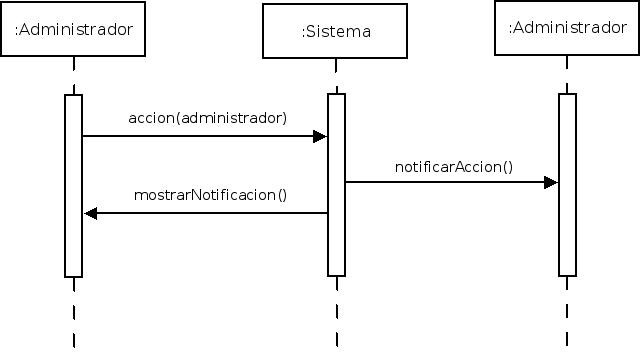
\includegraphics[scale=.50]{img/secuencias/gestion-administradores-activar-suspender.jpeg}
  \caption{Diagrama de secuencia: Gestión de administradores: Activar/Suspender administrador}
  \label{fig:secuencia-gestion-administradores-activar-suspender}
\end{figure}

\textbf{Contrato de operación: accion(administrador)}
\begin{itemize}
\item \textbf{Referencias cruzadas:} UC-25 (Cuadro \ref{tab:CU-activar-suspender-admin}).
\item \textbf{Responsabilidades:} El administrador podrá activar o suspender a otro administrador seleccionado.
\item \textbf{Precondiciones:} 
 \begin{itemize}
\item El administrador se ha identificado en el sistema previamente.
\item El administrador seleccionado debe estar activo para ser suspendido o viceversa.
\end {itemize}
\item \textbf{Postcondiciones:} 
 \begin{itemize}
\item Se realizará la acción seleccionada por el administrador \textit{(activar, suspender)} referente a otro administrador específico.
\end {itemize}
\end {itemize}

\textbf{Contrato de operación: notificarAccion()}
\begin{itemize}
\item \textbf{Referencias cruzadas:} UC-25 (Cuadro \ref{tab:CU-activar-suspender-admin}).
\item \textbf{Responsabilidades:} Mandar una notificación de suspensión/activación de la cuenta al administrador.
\item \textbf{Precondiciones:} 
 \begin{itemize}
\item Se ha suspendido/activado la cuenta de un administrador.
\end {itemize}
\item \textbf{Postcondiciones:} 
 \begin{itemize}
\item Se creará una nueva notificación de activación o suspensión de cuenta para el administrador seleccionado.
\end {itemize}
\end {itemize}

\textbf{Contrato de operación: mostrarNotificacion()}
\begin{itemize}
\item \textbf{Referencias cruzadas:} UC-25 (Cuadro \ref{tab:CU-activar-suspender-admin}).
\item \textbf{Responsabilidades:} Se mostrará un mensaje de acción por pantalla.
\item \textbf{Precondiciones:} 
 \begin{itemize}
\item Se ha realizado la acción correspondiente para activar el mensaje.
\end {itemize}
\item \textbf{Postcondiciones:} 
 \begin{itemize}
\item Se muestra el mensaje correspondiente a la acción en la pantalla, a modo de notificación para el administrador. Este puede ser confirmación de la acción o algún tipo de error en la ejecución de la misma.
\end {itemize}
\end {itemize}


\vspace{10mm}

\begin{figure}[H]
\centering
  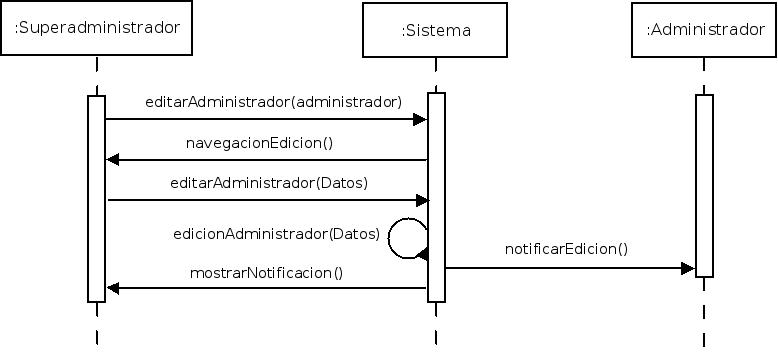
\includegraphics[scale=.50]{img/secuencias/gestion-administradores-editar-administrador.jpeg}
  \caption{Diagrama de secuencia: Gestión de administradores: Editar administrador}
  \label{fig:secuencia-gestion-administradores-editar-administrador}
\end{figure}

\textbf{Contrato de operación: editarAdministrador(administrador)}
\begin{itemize}
\item \textbf{Referencias cruzadas:} UC-26 (Cuadro \ref{tab:CU-editar-admin}).
\item \textbf{Responsabilidades:} Se informará al sistema de la acción de edición de un administrador específico por parte del superadministrador.
\item \textbf{Precondiciones:} 
 \begin{itemize}
\item El superadministrador se ha identificado en el sistema previamente.
\end {itemize}
\item \textbf{Postcondiciones:} 
 \begin{itemize}
\item Se manda la solicitud de edición del administrador seleccionado.
\end {itemize}
\end {itemize}

\textbf{Contrato de operación: navegacionEdicion()}
\begin{itemize}
\item \textbf{Referencias cruzadas:} UC-26 (Cuadro \ref{tab:CU-editar-admin}).
\item \textbf{Responsabilidades:} El sistema mostrará la página correspondiente a la edición de los datos del administrador.
\item \textbf{Precondiciones:} 
 \begin{itemize}
\item Se ha realizado la acción correspondiente para activar la navegación.
\end {itemize}
\item \textbf{Postcondiciones:} 
 \begin{itemize}
\item Se mostrará la página de edición del perfil del administrador seleccionado.
\end {itemize}
\end {itemize}

\textbf{Contrato de operación: editarAdministrador(Datos)}
\begin{itemize}
\item \textbf{Referencias cruzadas:} UC-26 (Cuadro \ref{tab:CU-editar-admin}).
\item \textbf{Responsabilidades:} Se mandará al sistema los datos del administrador para que este sea editado.
\item \textbf{Precondiciones:} 
 \begin{itemize}
\item El superadministrador se ha identificado en el sistema previamente.
\end {itemize}
\item \textbf{Postcondiciones:} 
 \begin{itemize}
\item Se envía el formulario de datos del administrador a editar al sistema.
\end {itemize}
\end {itemize}

\textbf{Contrato de operación: edicionAdministrador(Datos)}
\begin{itemize}
\item \textbf{Referencias cruzadas:} UC-26 (Cuadro \ref{tab:CU-editar-admin}).
\item \textbf{Responsabilidades:} Se realizará la edición de los datos del administrador, guardándolos en el sistema.
\item \textbf{Precondiciones:} 
 \begin{itemize}
\item Se ha enviado el formulario con los datos a editar.
\end {itemize}
\item \textbf{Postcondiciones:} 
 \begin{itemize}
\item El sistema guarda los datos recibidos para el administrador específico en la base de datos.
\end {itemize}
\end {itemize}

\textbf{Contrato de operación: notificarEdicion()}
\begin{itemize}
\item \textbf{Referencias cruzadas:} UC-26 (Cuadro \ref{tab:CU-editar-admin}).
\item \textbf{Responsabilidades:} Mandar una notificación de edición del perfil por parte del superadministrador al administrador.
\item \textbf{Precondiciones:} 
 \begin{itemize}
\item Se ha editado los datos del administrador por parte del superadministrador.
\end {itemize}
\item \textbf{Postcondiciones:} 
 \begin{itemize}
\item Se creará una nueva notificación de edición del perfil para el administrador seleccionado, indicando quién lo ha modificado.
\end {itemize}
\end {itemize}

\textbf{Contrato de operación: mostrarNotificacion()}
\begin{itemize}
\item \textbf{Referencias cruzadas:} UC-26 (Cuadro \ref{tab:CU-editar-admin}).
\item \textbf{Responsabilidades:} Se mostrará un mensaje de acción por pantalla.
\item \textbf{Precondiciones:} 
 \begin{itemize}
\item Se ha realizado la acción correspondiente para activar el mensaje.
\end {itemize}
\item \textbf{Postcondiciones:} 
 \begin{itemize}
\item Se muestra el mensaje correspondiente a la acción en la pantalla, a modo de notificación para el superadministrador. Este puede ser confirmación de la acción o algún tipo de error en la ejecución de la misma.
\end {itemize}
\end {itemize}


\vspace{10mm}

\begin{figure}[H]
\centering
  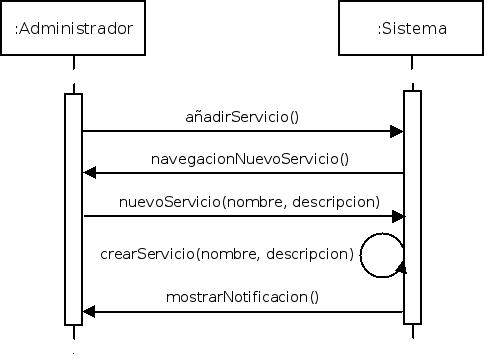
\includegraphics[scale=.55]{img/secuencias/gestion-servicios-alta-servicio.jpeg}
  \caption{Diagrama de secuencia: Gestión de servicios: Alta servicio}
  \label{fig:secuencia-gestion-servicios-alta-servicio}
\end{figure}

\textbf{Contrato de operación: añadirServicio()}
\begin{itemize}
\item \textbf{Referencias cruzadas:} UC-27 (Cuadro \ref{tab:CU-alta-servicio}).
\item \textbf{Responsabilidades:} Solicitar al sistema crear un nuevo servicio.
\item \textbf{Precondiciones:} 
 \begin{itemize}
\item El administrador se ha identificado en el sistema previamente.
\end {itemize}
\item \textbf{Postcondiciones:} 
 \begin{itemize}
\item Se enviará al sistema la solicitud de crear un nuevo servicio por parte del administrador.
\end {itemize}
\end {itemize}
\end{figure}

\textbf{Contrato de operación: navegacionNuevoServicio()}
\begin{itemize}
\item \textbf{Referencias cruzadas:} UC-27 (Cuadro \ref{tab:CU-alta-servicio}).
\item \textbf{Responsabilidades:} El sistema mostrará la ventana correspondiente a la creación de un nuevo servicio.
\item \textbf{Precondiciones:} 
 \begin{itemize}
\item Se ha realizado la acción correspondiente para activar la navegación.
\end {itemize}
\item \textbf{Postcondiciones:} 
 \begin{itemize}
\item Se mostrará la ventana de creación de un servicio nuevo en la interfaz del administrador.
\end {itemize}
\end {itemize}

\textbf{Contrato de operación: nuevoServicio(nombre, descripcion)}
\begin{itemize}
\item \textbf{Referencias cruzadas:} UC-27 (Cuadro \ref{tab:CU-alta-servicio}).
\item \textbf{Responsabilidades:} Se mandará al sistema los datos necesarios para la creación de un nuevo servicio.
\item \textbf{Precondiciones:} 
 \begin{itemize}
\item El administrador se ha identificado en el sistema previamente.
\end {itemize}
\item \textbf{Postcondiciones:} 
 \begin{itemize}
\item Se envía al sistema el nombre y la descripción del servicio a añadir.
\end {itemize}
\end {itemize}
\end{figure}

\textbf{Contrato de operación: crearServicio(nombre, descripcion)}
\begin{itemize}
\item \textbf{Referencias cruzadas:} UC-27 (Cuadro \ref{tab:CU-alta-servicio}).
\item \textbf{Responsabilidades:} Creación de un nuevo servicio con los datos recibidos.
\item \textbf{Precondiciones:} 
 \begin{itemize}
\item Se han recibido los datos de creación de un nuevo servicio.
\end {itemize}
\item \textbf{Postcondiciones:} 
 \begin{itemize}
 \item Se comprueban que el nombre del servicio es único.
\item Se crea un nuevo servicio y se introducen los datos en la base de datos.
\end {itemize}
\end {itemize}

\textbf{Contrato de operación: mostrarNotificacion()}
\begin{itemize}
\item \textbf{Referencias cruzadas:} UC-27 (Cuadro \ref{tab:CU-alta-servicio}).
\item \textbf{Responsabilidades:} Se mostrará un mensaje de acción por pantalla.
\item \textbf{Precondiciones:} 
 \begin{itemize}
\item Se ha realizado la acción correspondiente para activar el mensaje.
\end {itemize}
\item \textbf{Postcondiciones:} 
 \begin{itemize}
\item Se muestra el mensaje correspondiente a la acción en la pantalla, a modo de notificación para el administrador. Este puede ser confirmación de la acción o algún tipo de error en la ejecución de la misma.
\end {itemize}
\end {itemize}


\vspace{10mm}

\begin{figure}[H]
\centering
  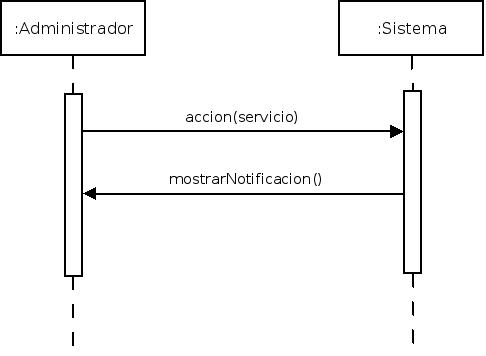
\includegraphics[scale=.55]{img/secuencias/gestion-servicios-suspender-activar-servicio.jpeg}
  \caption{Diagrama de secuencia: Gestión de servicios: Activar/Suspender servicio}
  \label{fig:secuencia-gestion-servicios-suspender-activar-servicio}
\end{figure}

\textbf{Contrato de operación: accion(servicio)}
\begin{itemize}
\item \textbf{Referencias cruzadas:} UC-28 (Cuadro \ref{tab:CU-activar-suspender-servicio}).
\item \textbf{Responsabilidades:} El administrador podrá activar o suspender el servicio seleccionado.
\item \textbf{Precondiciones:} 
 \begin{itemize}
\item El administrador se ha identificado en el sistema previamente.
\item El servicio seleccionado debe estar activo para ser suspendido o viceversa.
\end {itemize}
\item \textbf{Postcondiciones:} 
 \begin{itemize}
\item Se realizará la acción seleccionada por el administrador \textit{(activar, suspender)} referente a un servicio específico.
\end {itemize}
\end {itemize}

\textbf{Contrato de operación: mostrarNotificacion()}
\begin{itemize}
\item \textbf{Referencias cruzadas:} UC-28 (Cuadro \ref{tab:CU-activar-suspender-servicio}).
\item \textbf{Responsabilidades:} Se mostrará un mensaje de acción por pantalla.
\item \textbf{Precondiciones:} 
 \begin{itemize}
\item Se ha realizado la acción correspondiente para activar el mensaje.
\end {itemize}
\item \textbf{Postcondiciones:} 
 \begin{itemize}
\item Se muestra el mensaje correspondiente a la acción en la pantalla, a modo de notificación para el administrador. Este puede ser confirmación de la acción o algún tipo de error en la ejecución de la misma.
\end {itemize}
\end {itemize}


\vspace{10mm}

\begin{figure}[H]
\centering
  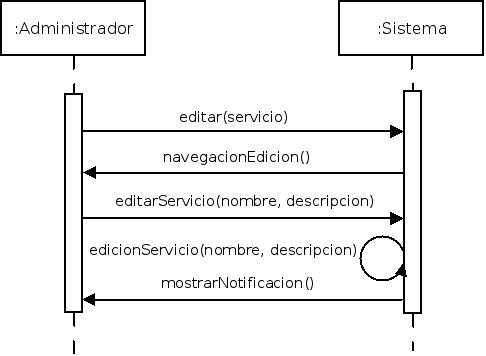
\includegraphics[scale=.55]{img/secuencias/gestion-servicios-editar-servicio.jpeg}
  \caption{Diagrama de secuencia: Gestión de servicios: Editar servicio}
  \label{fig:secuencia-gestion-servicios-editar-servicio}
\end{figure}

\textbf{Contrato de operación: editar(servicio)}
\begin{itemize}
\item \textbf{Referencias cruzadas:} UC-29 (Cuadro \ref{tab:CU-editar-servicio}).
\item \textbf{Responsabilidades:} Se solicitará al sistema la edición de un servicio específico por parte del administrador.
\item \textbf{Precondiciones:} 
 \begin{itemize}
\item El administrador se ha identificado en el sistema previamente.
\end {itemize}
\item \textbf{Postcondiciones:} 
 \begin{itemize}
\item Se manda la solicitud de edición del servicio seleccionado.
\end {itemize}
\end {itemize}

\textbf{Contrato de operación: navegacionEdicion()}
\begin{itemize}
\item \textbf{Referencias cruzadas:} UC-29 (Cuadro \ref{tab:CU-editar-servicio}).
\item \textbf{Responsabilidades:} El sistema mostrará la página correspondiente a la edición del servicio.
\item \textbf{Precondiciones:} 
 \begin{itemize}
\item Se ha realizado la acción correspondiente para activar la navegación.
\end {itemize}
\item \textbf{Postcondiciones:} 
 \begin{itemize}
\item Se mostrará la ventana de edición del servicio seleccionado.
\end {itemize}
\end {itemize}

\textbf{Contrato de operación: editarServicio(nombre, descripcion)}
\begin{itemize}
\item \textbf{Referencias cruzadas:} UC-29 (Cuadro \ref{tab:CU-editar-servicio}).
\item \textbf{Responsabilidades:} Se mandará al sistema los datos del servicio para que este sea editado.
\item \textbf{Precondiciones:} 
 \begin{itemize}
\item El administrador se ha identificado en el sistema previamente.
\end {itemize}
\item \textbf{Postcondiciones:} 
 \begin{itemize}
\item Se envía el nombre y la descripción del servicio a editar al sistema.
\end {itemize}
\end {itemize}

\textbf{Contrato de operación: edicionServicio(nombre, descripcion)}
\begin{itemize}
\item \textbf{Referencias cruzadas:} UC-29 (Cuadro \ref{tab:CU-editar-servicio}).
\item \textbf{Responsabilidades:} Se realizará la edición de los datos del servicio, guardándolos en el sistema.
\item \textbf{Precondiciones:} 
 \begin{itemize}
\item Se ha enviado el formulario con los datos a editar.
\end {itemize}
\item \textbf{Postcondiciones:} 
 \begin{itemize}
 \item Se comprueba que el nombre del servicio sea único.
\item El sistema guarda los datos recibidos para el servicio específico en la base de datos.
\end {itemize}
\end {itemize}

\textbf{Contrato de operación: mostrarNotificacion()}
\begin{itemize}
\item \textbf{Referencias cruzadas:} UC-29 (Cuadro \ref{tab:CU-editar-servicio}).
\item \textbf{Responsabilidades:} Se mostrará un mensaje de acción por pantalla.
\item \textbf{Precondiciones:} 
 \begin{itemize}
\item Se ha realizado la acción correspondiente para activar el mensaje.
\end {itemize}
\item \textbf{Postcondiciones:} 
 \begin{itemize}
\item Se muestra el mensaje correspondiente a la acción en la pantalla, a modo de notificación para el administrador. Este puede ser confirmación de la acción o algún tipo de error en la ejecución de la misma.
\end {itemize}
\end {itemize}


\vspace{10mm}

\begin{figure}[H]
\centering
  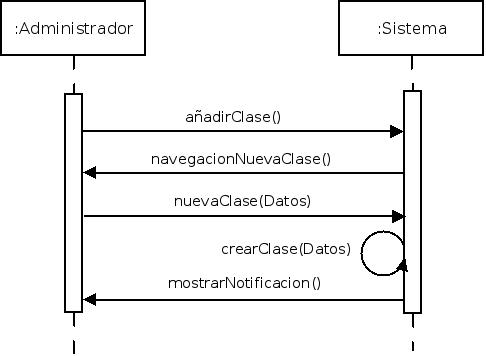
\includegraphics[scale=.55]{img/secuencias/gestion-servicios-alta-clase.jpeg}
  \caption{Diagrama de secuencia: Gestión de servicios: Alta clase}
  \label{fig:secuencia-gestion-servicios-alta-clase}
\end{figure}

\textbf{Contrato de operación: añadirClase()}
\begin{itemize}
\item \textbf{Referencias cruzadas:} UC-30 (Cuadro \ref{tab:CU-alta-clase}).
\item \textbf{Responsabilidades:} Solicitar al sistema crear una nueva clase.
\item \textbf{Precondiciones:} 
 \begin{itemize}
\item El administrador se ha identificado en el sistema previamente.
\end {itemize}
\item \textbf{Postcondiciones:} 
 \begin{itemize}
\item Se enviará al sistema la solicitud de crear una nueva clase por parte del administrador.
\end {itemize}
\end {itemize}
\end{figure}

\textbf{Contrato de operación: navegacionNuevaClase()}
\begin{itemize}
\item \textbf{Referencias cruzadas:} UC-30 (Cuadro \ref{tab:CU-alta-clase}).
\item \textbf{Responsabilidades:} El sistema navegará a la página correspondiente a la creación de una nueva clase.
\item \textbf{Precondiciones:} 
 \begin{itemize}
\item Se ha realizado la acción correspondiente para activar la navegación.
\end {itemize}
\item \textbf{Postcondiciones:} 
 \begin{itemize}
\item Se navegará a la página de creación de una clase nueva en la interfaz del administrador.
\end {itemize}
\end {itemize}

\textbf{Contrato de operación: nuevaClase(Datos)}
\begin{itemize}
\item \textbf{Referencias cruzadas:} UC-30 (Cuadro \ref{tab:CU-alta-clase}).
\item \textbf{Responsabilidades:} Se mandará al sistema los datos necesarios para la creación de una nueva clase.
\item \textbf{Precondiciones:} 
 \begin{itemize}
\item El administrador se ha identificado en el sistema previamente.
\end {itemize}
\item \textbf{Postcondiciones:} 
 \begin{itemize}
\item Se envía al sistema los datos de la clase a añadir.
\end {itemize}
\end {itemize}
\end{figure}

\textbf{Contrato de operación: crearClase(Datos)}
\begin{itemize}
\item \textbf{Referencias cruzadas:} UC-30 (Cuadro \ref{tab:CU-alta-clase}).
\item \textbf{Responsabilidades:} Creación de una nueva clase con los datos recibidos.
\item \textbf{Precondiciones:} 
 \begin{itemize}
\item Se han recibido los datos de creación de una nueva clase.
\end {itemize}
\item \textbf{Postcondiciones:} 
 \begin{itemize}
 \item Se comprueban que los datos recibidos son correctos.
\item Se crea una nueva clase y se introducen los datos en la base de datos.
\end {itemize}
\end {itemize}

\textbf{Contrato de operación: mostrarNotificacion()}
\begin{itemize}
\item \textbf{Referencias cruzadas:} UC-30 (Cuadro \ref{tab:CU-alta-clase}).
\item \textbf{Responsabilidades:} Se mostrará un mensaje de acción por pantalla.
\item \textbf{Precondiciones:} 
 \begin{itemize}
\item Se ha realizado la acción correspondiente para activar el mensaje.
\end {itemize}
\item \textbf{Postcondiciones:} 
 \begin{itemize}
\item Se muestra el mensaje correspondiente a la acción en la pantalla, a modo de notificación para el administrador. Este puede ser confirmación de la acción o algún tipo de error en la ejecución de la misma.
\end {itemize}
\end {itemize}


\vspace{10mm}

\begin{figure}[H]
\centering
  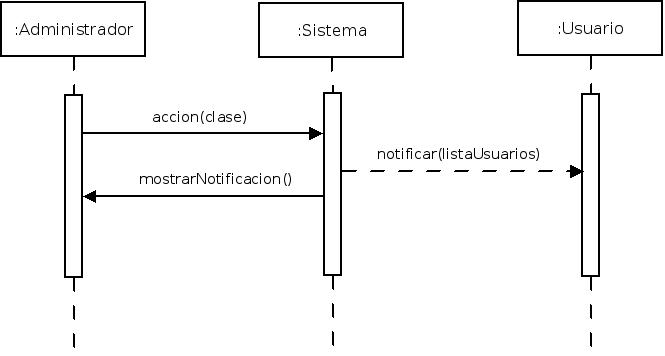
\includegraphics[scale=.55]{img/secuencias/gestion-servicios-suspender-activar-clase.jpeg}
  \caption{Diagrama de secuencia: Gestión de servicios: Activar/Suspender clase}
  \label{fig:secuencia-gestion-servicios-suspender-activar-clase}
\end{figure}

\textbf{Contrato de operación: accion(clase)}
\begin{itemize}
\item \textbf{Referencias cruzadas:} UC-31 (Cuadro \ref{tab:CU-activar-suspender-clase}).
\item \textbf{Responsabilidades:} El administrador podrá activar o suspender la clase seleccionada.
\item \textbf{Precondiciones:} 
 \begin{itemize}
\item El administrador se ha identificado en el sistema previamente.
\item La clase seleccionada debe estar activa para ser suspendida o viceversa.
\end {itemize}
\item \textbf{Postcondiciones:} 
 \begin{itemize}
\item Se realizará la acción seleccionada por el administrador \textit{(activar, suspender)} referente a una clase específica.
\end {itemize}
\end {itemize}

\textbf{Contrato de operación: notificar(listaUsuarios)}
\begin{itemize}
\item \textbf{Referencias cruzadas:} UC-31 (Cuadro \ref{tab:CU-activar-suspender-clase}).
\item \textbf{Responsabilidades:} Mandar una notificación de activación o suspensión de una clase específica por parte del administrador a todos los usuarios con reserva en la misma, en caso que existan.
\item \textbf{Precondiciones:} 
 \begin{itemize}
\item Se ha activado o suspendido una clase.
\end {itemize}
\item \textbf{Postcondiciones:} 
 \begin{itemize}
\item Se creará una nueva notificación de activación o suspensión de una determinada clase para cada uno de los usuarios con reserva en la misma.
\end {itemize}
\end {itemize}

\textbf{Contrato de operación: mostrarNotificacion()}
\begin{itemize}
\item \textbf{Referencias cruzadas:} UC-31 (Cuadro \ref{tab:CU-activar-suspender-clase}).
\item \textbf{Responsabilidades:} Se mostrará un mensaje de acción por pantalla.
\item \textbf{Precondiciones:} 
 \begin{itemize}
\item Se ha realizado la acción correspondiente para activar el mensaje.
\end {itemize}
\item \textbf{Postcondiciones:} 
 \begin{itemize}
\item Se muestra el mensaje correspondiente a la acción en la pantalla, a modo de notificación para el administrador. Este puede ser confirmación de la acción o algún tipo de error en la ejecución de la misma.
\end {itemize}
\end {itemize}


\vspace{10mm}

\begin{figure}[H]
\centering
  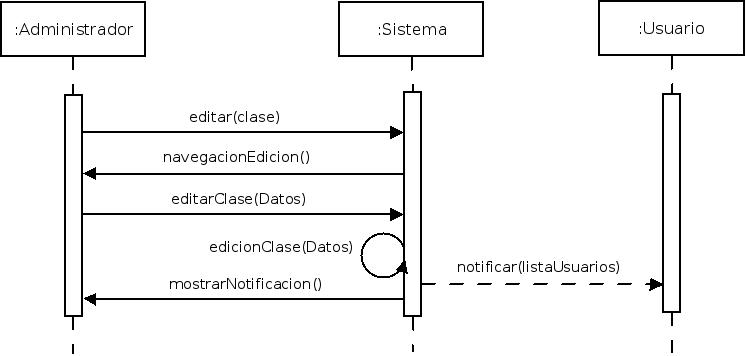
\includegraphics[scale=.50]{img/secuencias/gestion-servicios-editar-clase.jpeg}
  \caption{Diagrama de secuencia: Gestión de servicios: Editar clase}
  \label{fig:secuencia-editar-clase}
\end{figure}

\textbf{Contrato de operación: editar(clase)}
\begin{itemize}
\item \textbf{Referencias cruzadas:} UC-32 (Cuadro \ref{tab:CU-editar-clase}).
\item \textbf{Responsabilidades:} Se solicitará al sistema la edición de una clase específica por parte del administrador.
\item \textbf{Precondiciones:} 
 \begin{itemize}
\item El administrador se ha identificado en el sistema previamente.
\end {itemize}
\item \textbf{Postcondiciones:} 
 \begin{itemize}
\item Se manda la solicitud de edición de la clase seleccionada.
\end {itemize}
\end {itemize}

\textbf{Contrato de operación: navegacionEdicion()}
\begin{itemize}
\item \textbf{Referencias cruzadas:} UC-32 (Cuadro \ref{tab:CU-editar-clase}).
\item \textbf{Responsabilidades:} El sistema mostrará la página correspondiente a la edición de la clase.
\item \textbf{Precondiciones:} 
 \begin{itemize}
\item Se ha realizado la acción correspondiente para activar la navegación.
\end {itemize}
\item \textbf{Postcondiciones:} 
 \begin{itemize}
\item Se navegará a la página de edición de la clase seleccionada.
\end {itemize}
\end {itemize}

\textbf{Contrato de operación: editarClase(Datos)}
\begin{itemize}
\item \textbf{Referencias cruzadas:} UC-32 (Cuadro \ref{tab:CU-editar-clase}).
\item \textbf{Responsabilidades:} Se mandará al sistema los datos de la clase para que esta sea editada.
\item \textbf{Precondiciones:} 
 \begin{itemize}
\item El administrador se ha identificado en el sistema previamente.
\end {itemize}
\item \textbf{Postcondiciones:} 
 \begin{itemize}
\item Se envían todos los datos del formulario de edición de la clase al sistema.
\end {itemize}
\end {itemize}

\textbf{Contrato de operación: edicionClase(Datos)}
\begin{itemize}
\item \textbf{Referencias cruzadas:} UC-32 (Cuadro \ref{tab:CU-editar-clase}).
\item \textbf{Responsabilidades:} Se realizará la edición de los datos de la clase, guardándolos en el sistema.
\item \textbf{Precondiciones:} 
 \begin{itemize}
\item Se ha enviado el formulario con los datos a editar.
\end {itemize}
\item \textbf{Postcondiciones:} 
 \begin{itemize}
 \item Se comprueban que los datos recibidos son correctos.
\item El sistema guarda los datos recibidos para la clase específica en la base de datos.
\end {itemize}
\end {itemize}

\textbf{Contrato de operación: mostrarNotificacion()}
\begin{itemize}
\item \textbf{Referencias cruzadas:} UC-32 (Cuadro \ref{tab:CU-editar-clase}).
\item \textbf{Responsabilidades:} Se mostrará un mensaje de acción por pantalla.
\item \textbf{Precondiciones:} 
 \begin{itemize}
\item Se ha realizado la acción correspondiente para activar el mensaje.
\end {itemize}
\item \textbf{Postcondiciones:} 
 \begin{itemize}
\item Se muestra el mensaje correspondiente a la acción en la pantalla, a modo de notificación para el administrador. Este puede ser confirmación de la acción o algún tipo de error en la ejecución de la misma.
\end {itemize}
\end {itemize}


\vspace{10mm}

\begin{figure}[H]
\centering
  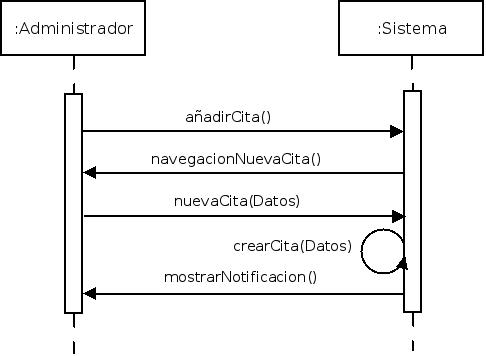
\includegraphics[scale=.55]{img/secuencias/gestion-servicios-alta-cita.jpeg}
  \caption{Diagrama de secuencia: Gestión de servicios: Alta cita}
  \label{fig:secuencia-gestion-servicios-alta-cita}
\end{figure}

\textbf{Contrato de operación: añadirCita()}
\begin{itemize}
\item \textbf{Referencias cruzadas:} UC-33 (Cuadro \ref{tab:CU-alta-cita}).
\item \textbf{Responsabilidades:} Solicitar al sistema crear una nueva cita.
\item \textbf{Precondiciones:} 
 \begin{itemize}
\item El administrador se ha identificado en el sistema previamente.
\end {itemize}
\item \textbf{Postcondiciones:} 
 \begin{itemize}
\item Se enviará al sistema la solicitud de crear una nueva cita por parte del administrador.
\end {itemize}
\end {itemize}
\end{figure}

\textbf{Contrato de operación: navegacionNuevaCita()}
\begin{itemize}
\item \textbf{Referencias cruzadas:} UC-33 (Cuadro \ref{tab:CU-alta-cita}).
\item \textbf{Responsabilidades:} El sistema navegará a la página correspondiente a la creación de una nueva cita.
\item \textbf{Precondiciones:} 
 \begin{itemize}
\item Se ha realizado la acción correspondiente para activar la navegación.
\end {itemize}
\item \textbf{Postcondiciones:} 
 \begin{itemize}
\item Se navegará a la página de creación de una cita nueva en la interfaz del administrador.
\end {itemize}
\end {itemize}

\textbf{Contrato de operación: nuevaCita(Datos)}
\begin{itemize}
\item \textbf{Referencias cruzadas:} UC-33 (Cuadro \ref{tab:CU-alta-cita}).
\item \textbf{Responsabilidades:} Se mandará al sistema los datos necesarios para la creación de una nueva cita.
\item \textbf{Precondiciones:} 
 \begin{itemize}
\item El administrador se ha identificado en el sistema previamente.
\end {itemize}
\item \textbf{Postcondiciones:} 
 \begin{itemize}
\item Se envía al sistema los datos de la cita a añadir.
\end {itemize}
\end {itemize}
\end{figure}

\textbf{Contrato de operación: crearCita(Datos)}
\begin{itemize}
\item \textbf{Referencias cruzadas:} UC-33 (Cuadro \ref{tab:CU-alta-cita}).
\item \textbf{Responsabilidades:} Creación de una nueva cita con los datos recibidos.
\item \textbf{Precondiciones:} 
 \begin{itemize}
\item Se han recibido los datos de creación de una nueva cita.
\end {itemize}
\item \textbf{Postcondiciones:} 
 \begin{itemize}
 \item Se comprueban que los datos recibidos son correctos.
\item Se crea una nueva cita y se introducen los datos en la base de datos.
\end {itemize}
\end {itemize}

\textbf{Contrato de operación: mostrarNotificacion()}
\begin{itemize}
\item \textbf{Referencias cruzadas:} UC-33 (Cuadro \ref{tab:CU-alta-cita}).
\item \textbf{Responsabilidades:} Se mostrará un mensaje de acción por pantalla.
\item \textbf{Precondiciones:} 
 \begin{itemize}
\item Se ha realizado la acción correspondiente para activar el mensaje.
\end {itemize}
\item \textbf{Postcondiciones:} 
 \begin{itemize}
\item Se muestra el mensaje correspondiente a la acción en la pantalla, a modo de notificación para el administrador. Este puede ser confirmación de la acción o algún tipo de error en la ejecución de la misma.
\end {itemize}
\end {itemize}


\vspace{10mm}

\begin{figure}[H]
\centering
  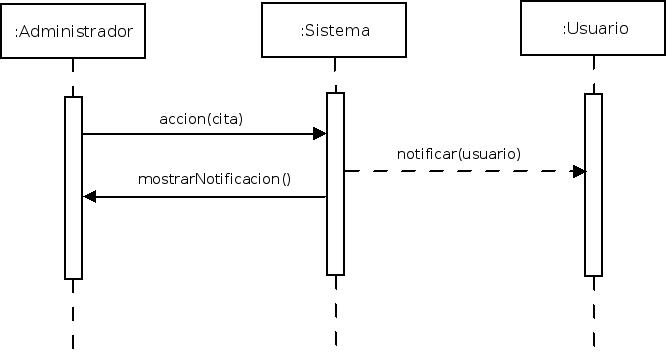
\includegraphics[scale=.55]{img/secuencias/gestion-servicios-suspender-activar-cita.jpeg}
  \caption{Diagrama de secuencia: Gestión de servicios: Activar/Suspender cita}
  \label{fig:secuencia-gestion-servicios-suspender-activar-cita}
\end{figure}

\textbf{Contrato de operación: accion(cita)}
\begin{itemize}
\item \textbf{Referencias cruzadas:} UC-34 (Cuadro \ref{tab:CU-activar-suspender-cita}).
\item \textbf{Responsabilidades:} El administrador podrá activar o suspender la cita seleccionada.
\item \textbf{Precondiciones:} 
 \begin{itemize}
\item El administrador se ha identificado en el sistema previamente.
\item La cita seleccionada debe estar activa para ser suspendida o viceversa.
\end {itemize}
\item \textbf{Postcondiciones:} 
 \begin{itemize}
\item Se realizará la acción seleccionada por el administrador \textit{(activar, suspender)} referente a una cita específica.
\end {itemize}
\end {itemize}

\textbf{Contrato de operación: notificar(listaUsuarios)}
\begin{itemize}
\item \textbf{Referencias cruzadas:} UC-34 (Cuadro \ref{tab:CU-activar-suspender-cita}).
\item \textbf{Responsabilidades:} Mandar una notificación de activación o suspensión de una cita específica por parte del administrador a todos los usuarios con reserva en la misma, en caso que existan.
\item \textbf{Precondiciones:} 
 \begin{itemize}
\item Se ha activado o suspendido una cita.
\end {itemize}
\item \textbf{Postcondiciones:} 
 \begin{itemize}
\item Se creará una nueva notificación de activación o suspensión de una determinada cita para cada uno de los usuarios con reserva en la misma.
\end {itemize}
\end {itemize}

\textbf{Contrato de operación: mostrarNotificacion()}
\begin{itemize}
\item \textbf{Referencias cruzadas:} UC-34 (Cuadro \ref{tab:CU-activar-suspender-cita}).
\item \textbf{Responsabilidades:} Se mostrará un mensaje de acción por pantalla.
\item \textbf{Precondiciones:} 
 \begin{itemize}
\item Se ha realizado la acción correspondiente para activar el mensaje.
\end {itemize}
\item \textbf{Postcondiciones:} 
 \begin{itemize}
\item Se muestra el mensaje correspondiente a la acción en la pantalla, a modo de notificación para el administrador. Este puede ser confirmación de la acción o algún tipo de error en la ejecución de la misma.
\end {itemize}
\end {itemize}


\vspace{10mm}

\begin{figure}[H]
\centering
  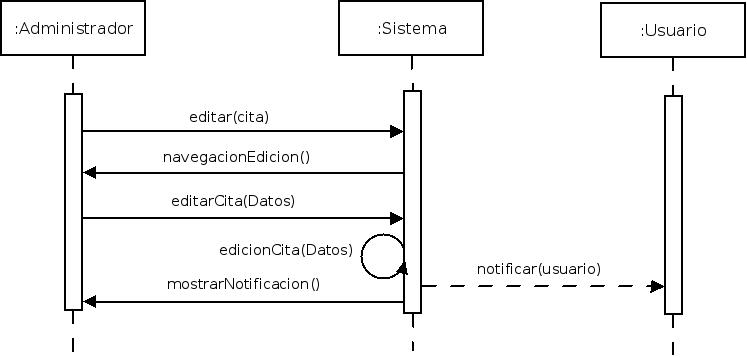
\includegraphics[scale=.50]{img/secuencias/gestion-servicios-editar-cita.jpeg}
  \caption{Diagrama de secuencia: Gestión de servicios: Editar cita}
  \label{fig:secuencia-gestion-servicios-editar-cita}
\end{figure}

\textbf{Contrato de operación: editar(cita)}
\begin{itemize}
\item \textbf{Referencias cruzadas:} UC-35 (Cuadro \ref{tab:CU-editar-cita}).
\item \textbf{Responsabilidades:} Se solicitará al sistema la edición de una cita específica por parte del administrador.
\item \textbf{Precondiciones:} 
 \begin{itemize}
\item El administrador se ha identificado en el sistema previamente.
\end {itemize}
\item \textbf{Postcondiciones:} 
 \begin{itemize}
\item Se manda la solicitud de edición de la cita seleccionada.
\end {itemize}
\end {itemize}

\textbf{Contrato de operación: navegacionEdicion()}
\begin{itemize}
\item \textbf{Referencias cruzadas:} UC-35 (Cuadro \ref{tab:CU-editar-cita}).
\item \textbf{Responsabilidades:} El sistema mostrará la página correspondiente a la edición de la cita.
\item \textbf{Precondiciones:} 
 \begin{itemize}
\item Se ha realizado la acción correspondiente para activar la navegación.
\end {itemize}
\item \textbf{Postcondiciones:} 
 \begin{itemize}
\item Se navegará a la página de edición de la cita seleccionada.
\end {itemize}
\end {itemize}

\textbf{Contrato de operación: editarCita(Datos)}
\begin{itemize}
\item \textbf{Referencias cruzadas:} UC-35 (Cuadro \ref{tab:CU-editar-cita}).
\item \textbf{Responsabilidades:} Se mandará al sistema los datos de la cita para que esta sea editada.
\item \textbf{Precondiciones:} 
 \begin{itemize}
\item El administrador se ha identificado en el sistema previamente.
\end {itemize}
\item \textbf{Postcondiciones:} 
 \begin{itemize}
\item Se envían todos los datos del formulario de edición de la cita al sistema.
\end {itemize}
\end {itemize}

\textbf{Contrato de operación: edicionCita(Datos)}
\begin{itemize}
\item \textbf{Referencias cruzadas:} UC-35 (Cuadro \ref{tab:CU-editar-cita}).
\item \textbf{Responsabilidades:} Se realizará la edición de los datos de la cita, guardándolos en el sistema.
\item \textbf{Precondiciones:} 
 \begin{itemize}
\item Se ha enviado el formulario con los datos a editar.
\end {itemize}
\item \textbf{Postcondiciones:} 
 \begin{itemize}
 \item Se comprueban que los datos recibidos son correctos.
\item El sistema guarda los datos recibidos para la cita específica en la base de datos.
\end {itemize}
\end {itemize}

\textbf{Contrato de operación: mostrarNotificacion()}
\begin{itemize}
\item \textbf{Referencias cruzadas:} UC-35 (Cuadro \ref{tab:CU-editar-cita}).
\item \textbf{Responsabilidades:} Se mostrará un mensaje de acción por pantalla.
\item \textbf{Precondiciones:} 
 \begin{itemize}
\item Se ha realizado la acción correspondiente para activar el mensaje.
\end {itemize}
\item \textbf{Postcondiciones:} 
 \begin{itemize}
\item Se muestra el mensaje correspondiente a la acción en la pantalla, a modo de notificación para el administrador. Este puede ser confirmación de la acción o algún tipo de error en la ejecución de la misma.
\end {itemize}
\end {itemize}


\vspace{10mm}

\begin{figure}[H]
\centering
  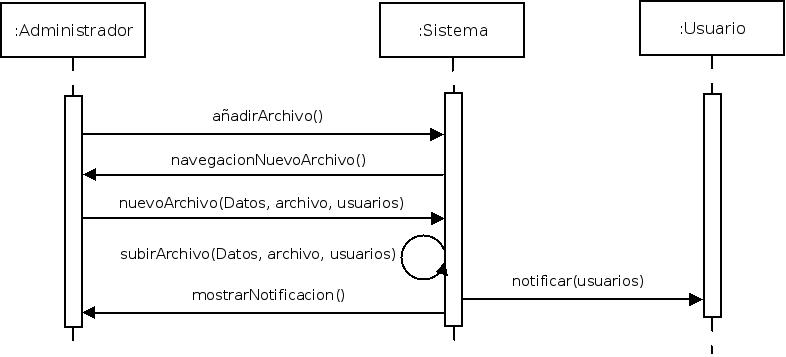
\includegraphics[scale=.50]{img/secuencias/gestion-servicios-subir-archivo.jpeg}
  \caption{Diagrama de secuencia: Gestión de servicios: Subir archivo}
  \label{fig:secuencia-gestion-servicios-subir-archivo}
\end{figure}

\textbf{Contrato de operación: añadirArchivo()}
\begin{itemize}
\item \textbf{Referencias cruzadas:} UC-36 (Cuadro \ref{tab:CU-subir-archivo}).
\item \textbf{Responsabilidades:} Solicitar al sistema subir un archivo.
\item \textbf{Precondiciones:} 
 \begin{itemize}
\item El administrador se ha identificado en el sistema previamente.
\end {itemize}
\item \textbf{Postcondiciones:} 
 \begin{itemize}
\item Se enviará al sistema la solicitud de subir un documento por parte del administrador.
\end {itemize}
\end {itemize}
\end{figure}

\textbf{Contrato de operación: navegacionNuevoArchivo()}
\begin{itemize}
\item \textbf{Referencias cruzadas:} UC-36 (Cuadro \ref{tab:CU-subir-archivo}).
\item \textbf{Responsabilidades:} El sistema mostrará la ventana correspondiente a la subida de un nuevo archivo.
\item \textbf{Precondiciones:} 
 \begin{itemize}
\item Se ha realizado la acción correspondiente para activar la navegación.
\end {itemize}
\item \textbf{Postcondiciones:} 
 \begin{itemize}
\item Se mostrará la ventana de subida de un nuevo archivo en la interfaz del administrador.
\end {itemize}
\end {itemize}

\textbf{Contrato de operación: nuevoArchivo(Datos, archivo, usuarios)}
\begin{itemize}
\item \textbf{Referencias cruzadas:} UC-36 (Cuadro \ref{tab:CU-subir-archivo}).
\item \textbf{Responsabilidades:} Se mandará al sistema los datos necesarios para subir el archivo.
\item \textbf{Precondiciones:} 
 \begin{itemize}
\item El administrador se ha identificado en el sistema previamente.
\end {itemize}
\item \textbf{Postcondiciones:} 
 \begin{itemize}
\item Se envía al sistema los datos del archivo a subir, el propio archivo y el usuario o lista de usuarios a los que el documento va destinado.
\end {itemize}
\end {itemize}
\end{figure}

\textbf{Contrato de operación: subirArchivo(Datos, archivo, usuarios)}
\begin{itemize}
\item \textbf{Referencias cruzadas:} UC-36 (Cuadro \ref{tab:CU-subir-archivo}).
\item \textbf{Responsabilidades:} Almacenamiento de una nuevo archivo, con los datos y archivo recibidos.
\item \textbf{Precondiciones:} 
 \begin{itemize}
\item Se han recibido los datos y el archivo para la creación de un documento nuevo.
\end {itemize}
\item \textbf{Postcondiciones:} 
 \begin{itemize}
 \item Se comprueban que los datos recibidos y el archivo son correctos.
\item Se crea y almacena un nuevo archivo y se introducen los datos en la base de datos.
\item Se especifica qué usuarios tienen acceso al archivo para su posterior consulta o descarga.
\end {itemize}
\end {itemize}

\textbf{Contrato de operación: notificar(usuarios)}
\begin{itemize}
\item \textbf{Referencias cruzadas:} UC-36 (Cuadro \ref{tab:CU-subir-archivo}).
\item \textbf{Responsabilidades:} Mandar una notificación de documento disponible a los usuarios especificados al subir el archivo, en caso que existan.
\item \textbf{Precondiciones:} 
 \begin{itemize}
\item Se ha subido al sistema un nuevo documento.
\end {itemize}
\item \textbf{Postcondiciones:} 
 \begin{itemize}
\item Se creará una nueva notificación de archivo subido disponible para cada uno de los usuarios especificados por el administrador en el proceso de subida.
\end {itemize}
\end {itemize}

\textbf{Contrato de operación: mostrarNotificacion()}
\begin{itemize}
\item \textbf{Referencias cruzadas:} UC-36 (Cuadro \ref{tab:CU-subir-archivo}).
\item \textbf{Responsabilidades:} Se mostrará un mensaje de acción por pantalla.
\item \textbf{Precondiciones:} 
 \begin{itemize}
\item Se ha realizado la acción correspondiente para activar el mensaje.
\end {itemize}
\item \textbf{Postcondiciones:} 
 \begin{itemize}
\item Se muestra el mensaje correspondiente a la acción en la pantalla, a modo de notificación para el administrador. Este puede ser confirmación de la acción o algún tipo de error en la ejecución de la misma.
\end {itemize}
\end {itemize}


\vspace{10mm}

\begin{figure}[H]
\centering
  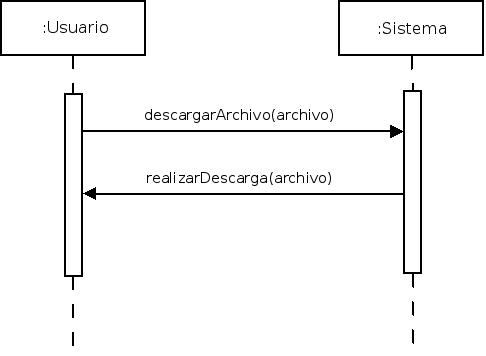
\includegraphics[scale=.55]{img/secuencias/gestion-servicios-descargar-archivo.jpeg}
  \caption{Diagrama de secuencia: Gestión de servicios: Descargar archivo}
  \label{fig:secuencia-gestion-servicios-descargar-archivo}
\end{figure}

\textbf{Contrato de operación: descargarArchivo(archivo)}
\begin{itemize}
\item \textbf{Referencias cruzadas:} UC-37 (Cuadro \ref{tab:CU-descargar-archivo}).
\item \textbf{Responsabilidades:} Solicitar al sistema la descarga del archivo seleccionado.
\item \textbf{Precondiciones:} 
 \begin{itemize}
\item El usuario se ha identificado en el sistema previamente.
\item Existen documentos subidos destinados al usuario.
\end {itemize}
\item \textbf{Postcondiciones:} 
 \begin{itemize}
\item El usuario manda al sistema la solicitud de descarga de un archivo específico.
\end {itemize}
\end {itemize}

\textbf{Contrato de operación: realizarDescarga(archivo)}
\begin{itemize}
\item \textbf{Referencias cruzadas:} UC-37 (Cuadro \ref{tab:CU-descargar-archivo}).
\item \textbf{Responsabilidades:} Realizar la descarga del documento seleccionado al dispositivo del usuario.
\item \textbf{Precondiciones:} 
 \begin{itemize}
\item El usuario ha solicitado la descarga de un archivo específico.
\end {itemize}
\item \textbf{Postcondiciones:} 
 \begin{itemize}
\item El documento seleccionado se descargará al dispositivo del usuario.
\end {itemize}
\end {itemize}


\vspace{10mm}

\begin{figure}[H]
\centering
  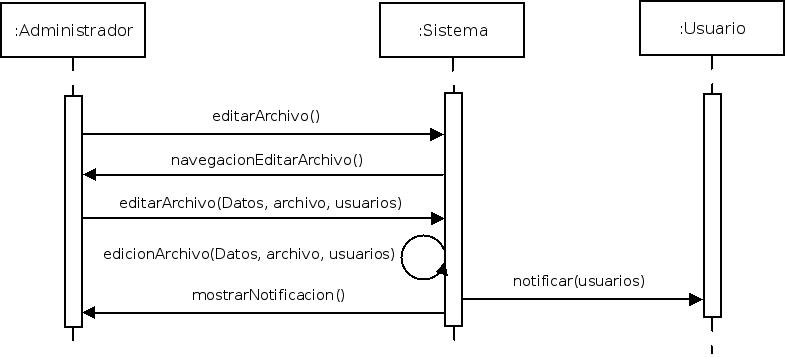
\includegraphics[scale=.50]{img/secuencias/gestion-servicios-editar-archivo.jpeg}
  \caption{Diagrama de secuencia: Gestión de servicios: Editar archivo}
  \label{fig:secuencia-gestion-servicios-editar-archivo}
\end{figure}

\textbf{Contrato de operación: editar(archivo)}
\begin{itemize}
\item \textbf{Referencias cruzadas:} UC-38 (Cuadro \ref{tab:CU-editar-archivo}).
\item \textbf{Responsabilidades:} Se solicitará al sistema la edición de un archivo específico por parte del administrador.
\item \textbf{Precondiciones:} 
 \begin{itemize}
\item El administrador se ha identificado en el sistema previamente.
\item Existen documentos subidos.
\end {itemize}
\item \textbf{Postcondiciones:} 
 \begin{itemize}
\item Se manda la solicitud de edición del archivo seleccionado.
\end {itemize}
\end {itemize}

\textbf{Contrato de operación: navegacionEdicion()}
\begin{itemize}
\item \textbf{Referencias cruzadas:} UC-38 (Cuadro \ref{tab:CU-editar-archivo}).
\item \textbf{Responsabilidades:} El sistema mostrará la página correspondiente a la edición del archivo.
\item \textbf{Precondiciones:} 
 \begin{itemize}
\item Se ha realizado la acción correspondiente para activar la navegación.
\end {itemize}
\item \textbf{Postcondiciones:} 
 \begin{itemize}
\item Se mostrará la ventana de edición del archivo seleccionado.
\end {itemize}
\end {itemize}

\textbf{Contrato de operación: editarArchivo(Datos, usuarios)}
\begin{itemize}
\item \textbf{Referencias cruzadas:} UC-38 (Cuadro \ref{tab:CU-editar-archivo}).
\item \textbf{Responsabilidades:} Se mandará al sistema los datos del archivo y usuarios a los que va destinado para que sea editado.
\item \textbf{Precondiciones:} 
 \begin{itemize}
\item El administrador se ha identificado en el sistema previamente.
\end {itemize}
\item \textbf{Postcondiciones:} 
 \begin{itemize}
\item Se envían todos los datos del formulario de edición del archivo al sistema.
\item Se especifican todos los usuarios que tendrán acceso al documento.
\end {itemize}
\end {itemize}

\textbf{Contrato de operación: edicionArchivo(Datos)}
\begin{itemize}
\item \textbf{Referencias cruzadas:} UC-38 (Cuadro \ref{tab:CU-editar-archivo}).
\item \textbf{Responsabilidades:} Se realizará la edición de los datos del archivo y la lista de usuarios con permiso para su acceso, guardándolos en el sistema.
\item \textbf{Precondiciones:} 
 \begin{itemize}
\item Se ha enviado el formulario con los datos a editar y la lista de usuarios a los que el documento va destinado.
\end {itemize}
\item \textbf{Postcondiciones:} 
 \begin{itemize}
 \item Se comprueban que los datos recibidos son correctos.
\item El sistema guarda los datos recibidos para el archivo específico en la base de datos.
\item El sistema da autorización a los usuarios especificados para que tengan acceso al archivo.
\end {itemize}
\end {itemize}

\textbf{Contrato de operación: notificar(usuarios)}
\begin{itemize}
\item \textbf{Referencias cruzadas:} UC-38 (Cuadro \ref{tab:CU-editar-archivo}).
\item \textbf{Responsabilidades:} Mandar una notificación de documento editado a los usuarios especificados con acceso al archivo, en caso que existan.
\item \textbf{Precondiciones:} 
 \begin{itemize}
\item Se ha editado un documento.
\end {itemize}
\item \textbf{Postcondiciones:} 
 \begin{itemize}
\item Se creará una nueva notificación de archivo editado disponible para cada uno de los usuarios especificados por el administrador en el proceso de edición.
\end {itemize}
\end {itemize}

\textbf{Contrato de operación: mostrarNotificacion()}
\begin{itemize}
\item \textbf{Referencias cruzadas:} UC-38 (Cuadro \ref{tab:CU-editar-archivo}).
\item \textbf{Responsabilidades:} Se mostrará un mensaje de acción por pantalla.
\item \textbf{Precondiciones:} 
 \begin{itemize}
\item Se ha realizado la acción correspondiente para activar el mensaje.
\end {itemize}
\item \textbf{Postcondiciones:} 
 \begin{itemize}
\item Se muestra el mensaje correspondiente a la acción en la pantalla, a modo de notificación para el administrador. Este puede ser confirmación de la acción o algún tipo de error en la ejecución de la misma.
\end {itemize}
\end {itemize}


\vspace{10mm}

\begin{figure}[H]
\centering
  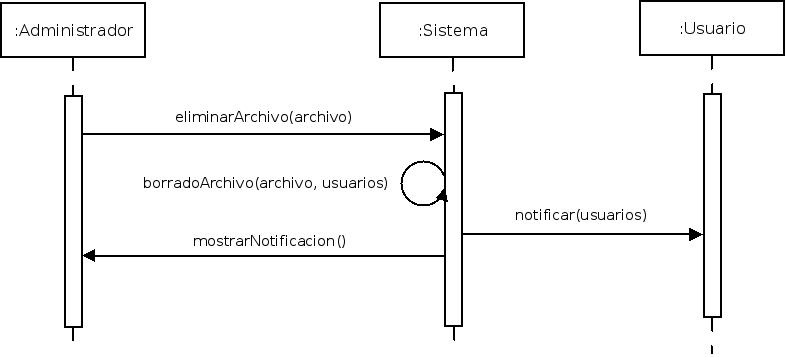
\includegraphics[scale=.50]{img/secuencias/gestion-servicios-eliminar-archivo.jpeg}
  \caption{Diagrama de secuencia: Gestión de servicios: Eliminar archivo}
  \label{fig:secuencia-gestion-servicios-eliminar-archivo}
\end{figure}

\textbf{Contrato de operación: eliminarArchivo(archivo)}
\begin{itemize}
\item \textbf{Referencias cruzadas:} UC-39 (Cuadro \ref{tab:CU-eliminar-archivo}).
\item \textbf{Responsabilidades:} Solicitar al sistema la eliminación del archivo seleccionado.
\item \textbf{Precondiciones:} 
 \begin{itemize}
\item El administrador se ha identificado en el sistema previamente.
\item Existen documentos subidos.
\end {itemize}
\item \textbf{Postcondiciones:} 
 \begin{itemize}
\item El usuario manda al sistema la solicitud de eliminación de un archivo específico.
\end {itemize}
\end {itemize}

\textbf{Contrato de operación: borradoArchivo(archivo)}
\begin{itemize}
\item \textbf{Referencias cruzadas:} UC-39 (Cuadro \ref{tab:CU-eliminar-archivo}).
\item \textbf{Responsabilidades:} Realizar la eliminación del documento seleccionado.
\item \textbf{Precondiciones:} 
 \begin{itemize}
\item El administrador ha solicitado la eliminación de un archivo específico.
\end {itemize}
\item \textbf{Postcondiciones:} 
 \begin{itemize}
\item Los datos del documento seleccionado se eliminarán de la base de datos y el propio archivo de donde esté almacenado.
\end {itemize}
\end {itemize}

\textbf{Contrato de operación: notificar(usuarios)}
\begin{itemize}
\item \textbf{Referencias cruzadas:} UC-39 (Cuadro \ref{tab:CU-eliminar-archivo}).
\item \textbf{Responsabilidades:} Mandar una notificación de documento eliminado a los usuarios con permisos para ver el archivo, en caso que existan.
\item \textbf{Precondiciones:} 
 \begin{itemize}
\item Se ha eliminado del sistema un documento.
\end {itemize}
\item \textbf{Postcondiciones:} 
 \begin{itemize}
\item Se creará una nueva notificación de archivo eliminado para cada uno de los usuarios con permisos de acceso al archivo, especificados por el administrador.
\end {itemize}
\end {itemize}

\textbf{Contrato de operación: mostrarNotificacion()}
\begin{itemize}
\item \textbf{Referencias cruzadas:} UC-39 (Cuadro \ref{tab:CU-eliminar-archivo}).
\item \textbf{Responsabilidades:} Se mostrará un mensaje de acción por pantalla.
\item \textbf{Precondiciones:} 
 \begin{itemize}
\item Se ha realizado la acción correspondiente para activar el mensaje.
\end {itemize}
\item \textbf{Postcondiciones:} 
 \begin{itemize}
\item Se muestra el mensaje correspondiente a la acción en la pantalla, a modo de notificación para el administrador. Este puede ser confirmación de la acción o algún tipo de error en la ejecución de la misma.
\end {itemize}
\end {itemize}


\vspace{10mm}

\begin{figure}[H]
\centering
  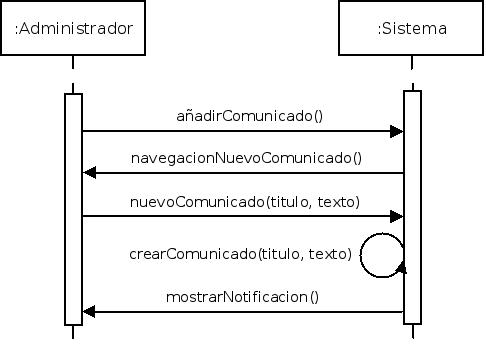
\includegraphics[scale=.55]{img/secuencias/nuevo-comunicado.jpeg}
  \caption{Diagrama de secuencia: Nuevo comunicado}
  \label{fig:secuencia-nuevo-comunicado}
\end{figure}

\textbf{Contrato de operación: añadirComunicado()}
\begin{itemize}
\item \textbf{Referencias cruzadas:} UC-40 (Cuadro \ref{tab:CU-nuevo-comunicado}).
\item \textbf{Responsabilidades:} Solicitar al sistema crear un nuevo comunicado.
\item \textbf{Precondiciones:} 
 \begin{itemize}
\item El administrador se ha identificado en el sistema previamente.
\end {itemize}
\item \textbf{Postcondiciones:} 
 \begin{itemize}
\item Se enviará al sistema la solicitud de crear un nuevo comunicado por parte del administrador.
\end {itemize}
\end {itemize}
\end{figure}

\textbf{Contrato de operación: navegacionNuevoComunicado()}
\begin{itemize}
\item \textbf{Referencias cruzadas:} UC-40 (Cuadro \ref{tab:CU-nuevo-comunicado}).
\item \textbf{Responsabilidades:} El sistema mostrará la página correspondiente a la creación de un nuevo comunicado.
\item \textbf{Precondiciones:} 
 \begin{itemize}
\item Se ha realizado la acción correspondiente para activar la navegación.
\end {itemize}
\item \textbf{Postcondiciones:} 
 \begin{itemize}
\item Se navegará a la página de creación de un comunicado nuevo en la interfaz del administrador.
\end {itemize}
\end {itemize}

\textbf{Contrato de operación: nuevoComunicado(titulo, texto)}
\begin{itemize}
\item \textbf{Referencias cruzadas:} UC-40 (Cuadro \ref{tab:CU-nuevo-comunicado}).
\item \textbf{Responsabilidades:} Se mandará al sistema los datos necesarios para la creación de un nuevo comunicado.
\item \textbf{Precondiciones:} 
 \begin{itemize}
\item El administrador se ha identificado en el sistema previamente.
\end {itemize}
\item \textbf{Postcondiciones:} 
 \begin{itemize}
\item Se envía al sistema el título y el texto del comunicado a añadir.
\end {itemize}
\end {itemize}
\end{figure}

\textbf{Contrato de operación: crearComunicado(titulo, texto)}
\begin{itemize}
\item \textbf{Referencias cruzadas:} UC-40 (Cuadro \ref{tab:CU-nuevo-comunicado}).
\item \textbf{Responsabilidades:} Creación de un nuevo comunicado con los datos recibidos.
\item \textbf{Precondiciones:} 
 \begin{itemize}
\item Se han recibido los datos de creación de un nuevo comunicado.
\end {itemize}
\item \textbf{Postcondiciones:} 
 \begin{itemize}
\item Se crea un nuevo comunicado y se introducen los datos en la base de datos.
\end {itemize}
\end {itemize}

\textbf{Contrato de operación: mostrarNotificacion()}
\begin{itemize}
\item \textbf{Referencias cruzadas:} UC-40 (Cuadro \ref{tab:CU-nuevo-comunicado}).
\item \textbf{Responsabilidades:} Se mostrará un mensaje de acción por pantalla.
\item \textbf{Precondiciones:} 
 \begin{itemize}
\item Se ha realizado la acción correspondiente para activar el mensaje.
\end {itemize}
\item \textbf{Postcondiciones:} 
 \begin{itemize}
\item Se muestra el mensaje correspondiente a la acción en la pantalla, a modo de notificación para el administrador. Este puede ser confirmación de la acción o algún tipo de error en la ejecución de la misma.
\end {itemize}
\end {itemize}


\vspace{10mm}

\begin{figure}[H]
\centering
  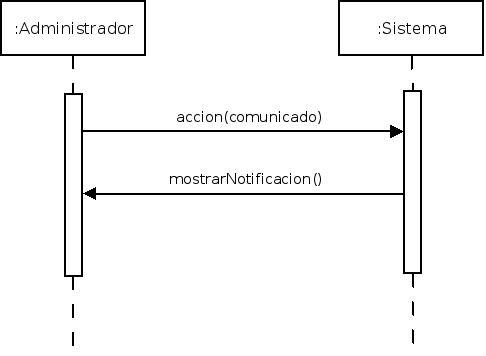
\includegraphics[scale=.55]{img/secuencias/suspender-activar-comunicado.jpeg}
  \caption{Diagrama de secuencia: Activar/Suspender comunicado}
  \label{fig:secuencia-suspender-activar-comunicado}
\end{figure}

\textbf{Contrato de operación: accion(comunicado)}
\begin{itemize}
\item \textbf{Referencias cruzadas:} UC-41 (Cuadro \ref{tab:CU-activar-suspender-comunicado}).
\item \textbf{Responsabilidades:} El administrador podrá activar o suspender el comunicado seleccionado.
\item \textbf{Precondiciones:} 
 \begin{itemize}
\item El administrador se ha identificado en el sistema previamente.
\item El comunicado seleccionado debe estar activo para ser suspendido o viceversa.
\end {itemize}
\item \textbf{Postcondiciones:} 
 \begin{itemize}
\item Se realizará la acción seleccionada por el administrador \textit{(activar, suspender)} referente a un comunicado específico.
\end {itemize}
\end {itemize}

\textbf{Contrato de operación: mostrarNotificacion()}
\begin{itemize}
\item \textbf{Referencias cruzadas:} UC-41 (Cuadro \ref{tab:CU-activar-suspender-comunicado}).
\item \textbf{Responsabilidades:} Se mostrará un mensaje de acción por pantalla.
\item \textbf{Precondiciones:} 
 \begin{itemize}
\item Se ha realizado la acción correspondiente para activar el mensaje.
\end {itemize}
\item \textbf{Postcondiciones:} 
 \begin{itemize}
\item Se muestra el mensaje correspondiente a la acción en la pantalla, a modo de notificación para el administrador. Este puede ser confirmación de la acción o algún tipo de error en la ejecución de la misma.
\end {itemize}
\end {itemize}


\vspace{10mm}

\begin{figure}[H]
\centering
  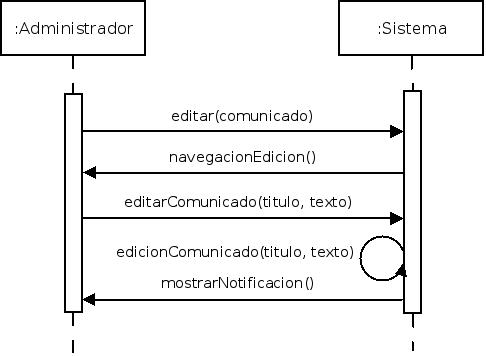
\includegraphics[scale=.55]{img/secuencias/editar-comunicado.jpeg}
  \caption{Diagrama de secuencia: Editar comunicado}
  \label{fig:secuencia-editar-comunicado}
\end{figure}

\textbf{Contrato de operación: editar(comunicado)}
\begin{itemize}
\item \textbf{Referencias cruzadas:} UC-42 (Cuadro \ref{tab:CU-editar-comunicado}).
\item \textbf{Responsabilidades:} Se solicitará al sistema la edición de un comunicado específico por parte del administrador.
\item \textbf{Precondiciones:} 
 \begin{itemize}
\item El administrador se ha identificado en el sistema previamente.
\end {itemize}
\item \textbf{Postcondiciones:} 
 \begin{itemize}
\item Se manda la solicitud de edición del comunicado seleccionado.
\end {itemize}
\end {itemize}

\textbf{Contrato de operación: navegacionEdicion()}
\begin{itemize}
\item \textbf{Referencias cruzadas:} UC-42 (Cuadro \ref{tab:CU-editar-comunicado}).
\item \textbf{Responsabilidades:} El sistema mostrará la página correspondiente a la edición del comunicado.
\item \textbf{Precondiciones:} 
 \begin{itemize}
\item Se ha realizado la acción correspondiente para activar la navegación.
\end {itemize}
\item \textbf{Postcondiciones:} 
 \begin{itemize}
\item Se navegará a la página de edición del comunicado seleccionado.
\end {itemize}
\end {itemize}

\textbf{Contrato de operación: editarComunicado(titulo, texto)}
\begin{itemize}
\item \textbf{Referencias cruzadas:} UC-42 (Cuadro \ref{tab:CU-editar-comunicado}).
\item \textbf{Responsabilidades:} Se mandará al sistema los datos del comunicado para que este sea editado.
\item \textbf{Precondiciones:} 
 \begin{itemize}
\item El administrador se ha identificado en el sistema previamente.
\end {itemize}
\item \textbf{Postcondiciones:} 
 \begin{itemize}
\item Se envía el nombre y la descripción del comunicado a editar al sistema.
\end {itemize}
\end {itemize}

\textbf{Contrato de operación: edicionComunicado(titulo, texto)}
\begin{itemize}
\item \textbf{Referencias cruzadas:} UC-42 (Cuadro \ref{tab:CU-editar-comunicado}).
\item \textbf{Responsabilidades:} Se realizará la edición de los datos del comunicado, guardándolos en el sistema.
\item \textbf{Precondiciones:} 
 \begin{itemize}
\item Se ha enviado el formulario con los datos a editar.
\end {itemize}
\item \textbf{Postcondiciones:} 
 \begin{itemize}
\item El sistema guarda los datos recibidos para el comunicado específico en la base de datos.
\end {itemize}
\end {itemize}

\textbf{Contrato de operación: mostrarNotificacion()}
\begin{itemize}
\item \textbf{Referencias cruzadas:} UC-42 (Cuadro \ref{tab:CU-editar-comunicado}).
\item \textbf{Responsabilidades:} Se mostrará un mensaje de acción por pantalla.
\item \textbf{Precondiciones:} 
 \begin{itemize}
\item Se ha realizado la acción correspondiente para activar el mensaje.
\end {itemize}
\item \textbf{Postcondiciones:} 
 \begin{itemize}
\item Se muestra el mensaje correspondiente a la acción en la pantalla, a modo de notificación para el administrador. Este puede ser confirmación de la acción o algún tipo de error en la ejecución de la misma.
\end {itemize}
\end {itemize}






\chapter{Diseño del Sistema}
% !TEX encoding = UTF-8 Unicode
% ------------------------------------------------------------------------------
% Este fichero es parte de la plantilla LaTeX para la realización de Proyectos
% Final de Grado, protegido bajo los términos de la licencia GFDL.
% Para más información, la licencia completa viene incluida en el
% fichero fdl-1.3.tex

% Copyright (C) 2012 SPI-FM. Universidad de Cádiz
% ------------------------------------------------------------------------------

A lo largo de este capítulo se detallará la arquitectura general del sistema de información, el diseño fí­sico de datos, el diseño detallado de componentes software y el diseño de la interfaz de usuario:

\section{Arquitectura del Sistema}

En esta sección se define la arquitectura general del sistema de información, especificando la infraestructura tecnológica necesaria para dar soporte al software y la estructura de los componentes que lo forman.


\subsection{Arquitectura Fí­sica} \label{sec:arquitectura-fisica}

El desarrollo de este proyecto no precisa de ningún elemento hardware adicional al equipo de trabajo del alumno. Se ha utilizado un portátil MacBook Pro de 15 pulgadas, con procesador Intel Core i7 de 2.2 GHz y 16GB de memoria RAM DDR3. Para la realización de pruebas, se usará tanto este equipo como otro portátil del propio alumno, donde se instalará todo el software requerido para comprobar que la instalación y ejecución de la aplicación responde adecuadamente en un equipo diferente. En este caso será un portátil Acer con procesador Dual Core, 4GB de memoria RAM y disco duro SSD. \\

Respecto al software, el MacBook trabaja bajo el sistema operativo macOS Sierra. Todo el proyecto se ha desarrollado utilizando el IDE NetBeans 8.0.2 y usando el servidor de aplicaciones GlassFish en un entorno local. Para la documentación, se ha utilizado TeXShop, como herramienta de edición para \LaTeX. Para las pruebas, el portátil a utilizar correrá bajo Windows 7, usando el mismo IDE y servidor de aplicaciones. \\

Respecto al entorno de producción, la aplicación web se alojará en un servidor que se contratará para tal fin. Por lo tanto, solo se requerirá acceso al servidor para la instalación de, en este caso, el servidor de aplicaciones Wildfly (JBoss) -habiendo sido probado previamente en entorno local de desarrollo-, siendo este similar a GlassFish, por lo que la aplicación apenas requerirá cambio alguno y aportará algo más de robustez y calidad. Los usuarios del sistema podrán hacer uso del mismo utilizando cualquier dispositivo con acceso a internet a través de un navegador web, como sus propios móviles, tablets o PCs. \\

En el apartado \ref{sec:entorno-construcción} se describirá detalladamente todo el software, lenguaje, frameworks, etc. utilizados para el desarrollo del sistema.


\subsection{Arquitectura Lógica} \label{sec:arquitectura-logica}

Para el desarrollo de esta aplicación web se ha utilizado una arquitectura de 3 capas, basada en el patrón de diseño Modelo-Vista-Controlador (MVC), donde la primera capa correspondería a la capa de usuario, la segunda la de negocio y por último la capa de datos.

\vspace{10mm}

\begin{figure}[H]
\centering
  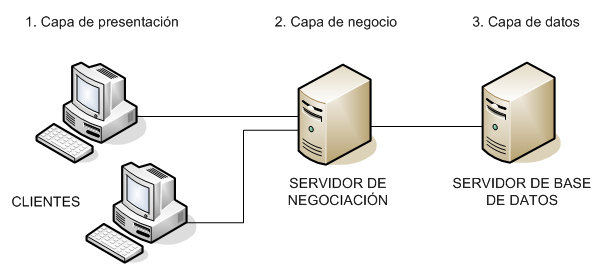
\includegraphics[scale=.55]{img/arquitectura-tres-capas.jpg}
  \caption{Representación de Arquitectura de 3 Capas}
  \label{fig:arquitectura-tres-capas}
\end{figure}

\vspace{10mm}

La programación por capas es un modelo de desarrollo software en el que el objetivo primordial es la separación (desacomplamiento) de las partes que componen un sistema software o también una arquitectura cliente-servidor: lógica de negocios, capa de presentación y capa de datos. De esta forma, por ejemplo, es sencillo y mantenible crear diferentes interfaces sobre un mismos sistema sin requerirse cambio alguno en la capa de datos o lógica.\\

La ventaja principal de este estilo es que el desarrollo se puede llevar a cabo en varios niveles y, en caso de que sobrevenga algún cambio, solo afectará al nivel requerido sin tener que revisar entre el código fuente de otros módulos (\ref{bio:wikipedia-programacion-por-capas}).

\paragraph*{Capa de presentación (frontend)}

Este grupo de artefactos software conforman la capa de presentación del sistema, incluyendo tanto los componentes de la vista como los elementos de control de la misma. \\

Es la capa que ve el usuario, denominada también \textit{capa de usuario}. Presenta el sistema al usuario, le comunica la información y captura la información del usuario en un mínimo de proceso (realiza un filtrado previo para comprobar que no hay errores de formato). También es conocida como interfaz gráfica y debe tener la característica de ser amigable (entendible y fácil de usar) para el usuario. Esta capa se comunica únicamente con la capa de negocio.

\paragraph*{Capa de negocio}

Esta capa recibe las peticiones del usuario y se envían las respuestas tras el proceso. Se denomina capa de negocio (o de lógica del negocio) porque es aquí donde se establecen todas las reglas que deben cumplirse. Esta capa se comunica con la capa de presentación, para recibir las solicitudes y presentar los resultados, y con la capa de datos, para solicitar al gestor de base de datos almacenar o recuperar datos de él. 

\paragraph*{Capa de persistencia}

Este grupo de artefactos software conforman la capa de integración del sistema, incluyendo las clases de abstracción para el acceso a datos.\\

Es donde residen los datos y es la encargada de acceder a los mismos. Está formada por un gestor de base de datos que realiza todo el almacenamiento de datos, recibe solicitudes de almacenamiento o recuperación de información desde la capa de negocio.\\

Es común que a la capa de negocio y de datos de los sistemas web se denomine conjuntamente como backend de la aplicación.\\

Como se ha comentado anteriormente, el patrón de diseño usado para el desarrollo del proyecto ha sido Modelo-Vista-Controlador, el cual separa los datos y la lógica de negocio de una aplicación de la interfaz de usuario y el módulo encargado de gestionar los eventos y las comunicaciones. Para ello MVC propone la construcción de tres componentes distintos que son el modelo, la vista y el controlador, es decir, por un lado define componentes para la representación de la información, y por otro lado para la interacción del usuario.​ Este patrón de arquitectura de software se basa en las ideas de reutilización de código y la separación de conceptos, características que buscan facilitar la tarea de desarrollo de aplicaciones y su posterior mantenimiento (\ref{bio:wikipedia-modelo-vista-controlador}).

\vspace{10mm}

\begin{figure}[H]
\centering
  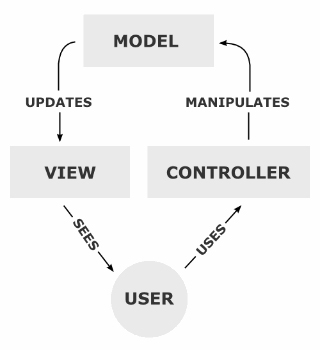
\includegraphics[scale=.55]{img/proceso-MVC.jpg}
  \caption{Proceso del Patrón MVC}
  \label{fig:proceso-MVC}
\end{figure}

\vspace{10mm}

\paragraph*{Modelo}

Es la representación de la información con la cual el sistema opera, por lo tanto gestiona todos los accesos a dicha información, tanto consultas como actualizaciones, implementando también los privilegios de acceso que se hayan descrito en las especificaciones de la aplicación (lógica de negocio). Envía a la \textit{vista} aquella parte de la información que en cada momento se le solicita para que sea mostrada al usuario. Las peticiones de acceso o manipulación de información llegan al \textit{modelo} a través del \textit{controlador}.

\paragraph*{Controlador}

Responde a eventos (acciones del usuario) e invoca peticiones al \textit{modelo} cuando se hace alguna solicitud sobre la información (por ejemplo, editar un documento o un registro en la base de datos). También puede enviar comandos a su \textit{vista} asociada si se solicita un cambio en la forma en que se presenta el \textit{modelo} (por ejemplo, desplazamiento o scroll por un documento o por los diferentes registros de una base de datos), por tanto se podría decir que el \textit{controlador} hace de intermediario entre la \textit{vista}  y el \textit{modelo}.

\paragraph*{Vista}

Presenta el \textit{modelo} (información y lógica de negocio) en un formato adecuado para interactuar (la interfaz de usuario), por tanto requiere de dicho \textit{modelo} la información que debe representar como salida.\\

Por tanto, aunque la arquitectura de 3 capas o niveles y el patrón MVC presenten sus similitudes y diferencias, cada uno tiene su función y son compatibles entre sí, de ahí el uso de ambos en el presente proyecto. A continuación, se presenta una gráfica comparativa de ambos modelos. 

\vspace{10mm}

\begin{figure}[H]
\centering
  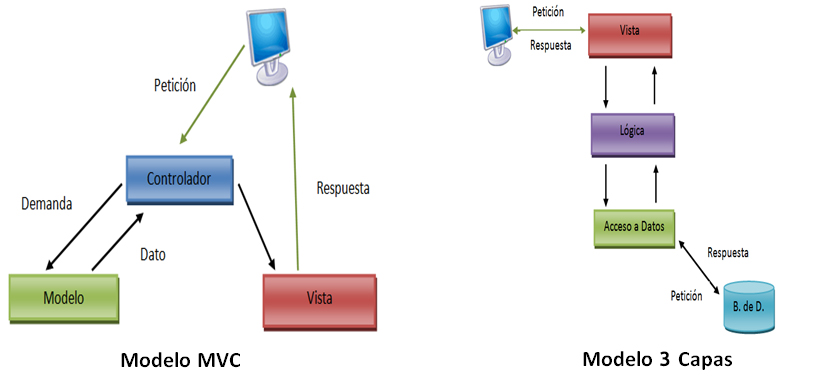
\includegraphics[scale=.50]{img/MVC-vs-3-capas.jpg}
  \caption{Comparativa entre modelo MVC y arquitectura de 3 capas}
  \label{fig:MVC-vs-3-capas}
\end{figure}

\vspace{10mm}


\section{Diseño Fí­sico de Datos}

Habiendo realizado previamente el modelo de conceptual de clases, detallado en la sección \ref{sec:modelo-conceptual}, se puede tener una idea de la estructura física que tendrá los datos en el sistema de gestión de base de datos (SGBD) a utilizar, en este caso PostgreSQL, teniendo en cuenta que aparecerán nuevas tablas en la BD provenientes de las relaciones entre las clases. Pero, por supuesto, hay que tener en cuenta que el acceso a los mismos se realice de una forma eficaz e independiente al resto de la implementación.\\ 

Y es por ello por lo que la arquitectura lógica del sistema se divide en 3 capas bien diferenciadas. La tercera de las capas contendrá el DAO (\textit{Data Access Object, Objeto de Acceso a Datos}), encargado del acceso a los datos físicos y única capa que realizará cambios en los mismos. Esto permite que si aflora la necesidad de cambios en la estructura de nuestros datos, o incluso cambiar de SGBD, las demás capas queden totalmente al margen de estos cambios, siendo un trámite independiente sin afectar -dependiendo del cambio, claro está- a la lógica de negocio o la interfaz de usuario. 


\section{Diseño de la Interfaz de Usuario} 

A continuación se muestra un prototipo de la interfaz de usuario del sistema para PC. Se mostrarán las páginas principales de la aplicación web de manera generalizada: Pantalla de registro de usuario, inicio de sesión, pantalla generalizada de la aplicación una vez iniciada la sesión y página con prototipo de tabla de datos (para listado de usuarios, servicios, clases, etc.). 


\vspace{10mm}

\begin{figure}[H]
\centering
  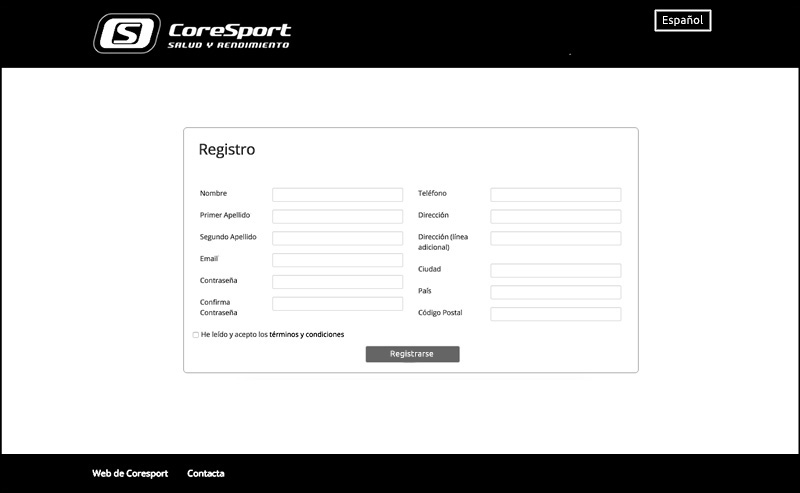
\includegraphics[scale=.40]{img/interfaz/registro.jpg}
  \caption{Interfaz de usuario: Registro}
  \label{fig:interfaz-registro}
\end{figure}

\begin{figure}[H]
\centering
  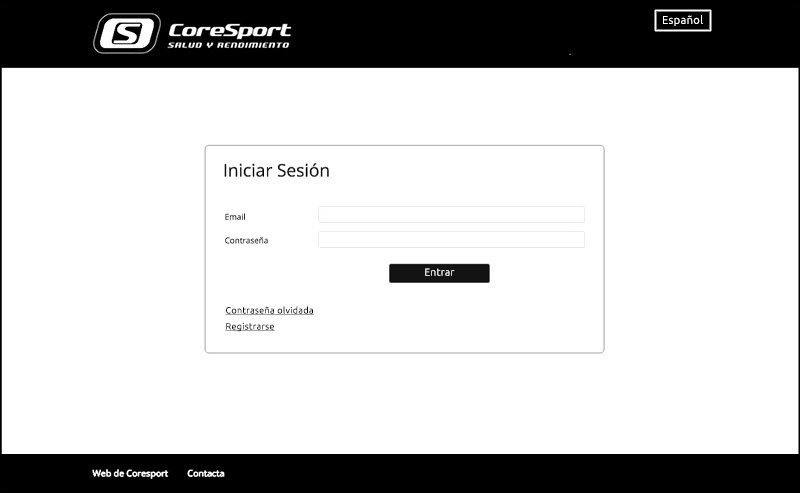
\includegraphics[scale=.40]{img/interfaz/inicio-sesion.jpg}
  \caption{Interfaz de usuario: Inicio de sesión}
  \label{fig:interfaz-inicio-sesion}
\end{figure}


\begin{figure}[H]
\centering
  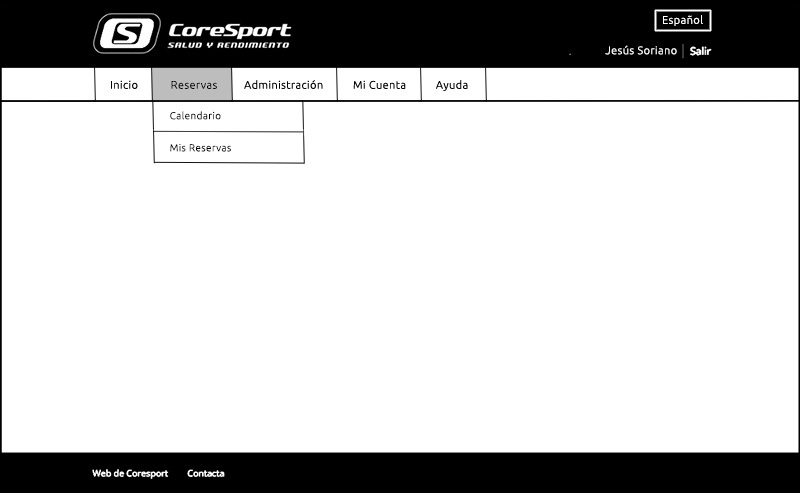
\includegraphics[scale=.40]{img/interfaz/pantalla-principal.jpg}
  \caption{Interfaz de usuario: Pantalla principal}
  \label{fig:interfaz-pantalla-principal}
\end{figure}

\begin{figure}[H]
\centering
  \includegraphics[scale=.40]{img/interfaz/cuadro-general.jpg}
  \caption{Interfaz de usuario: Pantalla con tabla de datos}
  \label{fig:interfaz-cuadro-general}
\end{figure}


Asimismo, se ha realizado el diseño de las pantallas para dispositivos de menor tamaño, al ser un diseño adaptativo dependiendo del mismo. A continuación se podrán visualizar los mockups realizados para la interfaz de dispositivos móviles. En este caso, las pantalla de inicio de sesión, pantalla general de usuario y menú desplegado.


\begin{figure}[H]
\centering
  \includegraphics[scale=.50]{img/interfaz/inicio-sesion-movil.jpg}
  \caption{Interfaz de usuario para dispositivos móviles: Inicio de sesión}
  \label{fig:interfaz-inicio-sesion-movil}
\end{figure}

\begin{figure}[H]
\centering
  \includegraphics[scale=.50]{img/interfaz/pantalla-principal-movil.jpg}
  \caption{Interfaz de usuario para dispositivos móviles: Pantalla principal}
  \label{fig:interfaz-pantalla-principal-movil}
\end{figure}

\begin{figure}[H]
\centering
  \includegraphics[scale=.50]{img/interfaz/menu-movil.jpg}
  \caption{Interfaz de usuario para dispositivos móviles: Menú desplegable}
  \label{fig:interfaz-menu-movil}
\end{figure}


Además, la figura \ref{fig:interfaz-navegacion} muestra el diagrama de navegación entre pantallas. Observamos que es una navegación sencilla; la página inicial sería la de registro de usuario, o inicio de sesión para usuarios registrados. A continuación, el sistema nos llevaría a la página de inicio, desde la que se podrá navegar, a través del menú y/o enlaces disponibles hasta las distintas vistas de la interfaz. En todo momento será posible cerrar la sesión del usuario, volviendo a la página de inicio de sesión, o cambiar el idioma de la interfaz mediante la opción destinada a ello en la parte superior derecha de la pantalla. 


Esta navegación ocurrirá de la misma manera en todo tipo de dispositivos, donde el único cambio sería el diseño de la pantalla, como hemos observado en los prototipos para PC y móvil.


\begin{figure}[H]
\centering
  \includegraphics[scale=.55]{img/interfaz/navegacion.jpg}
  \caption{Interfaz de usuario: Diagrama de navegación}
  \label{fig:interfaz-navegacion}
\end{figure}



\chapter{Construcción del Sistema}
% !TEX encoding = UTF-8 Unicode
% ------------------------------------------------------------------------------
% Este fichero es parte de la plantilla LaTeX para la realización de Proyectos
% Final de Grado, protegido bajo los términos de la licencia GFDL.
% Para más información, la licencia completa viene incluida en el
% fichero fdl-1.3.tex

% Copyright (C) 2012 SPI-FM. Universidad de Cádiz
% ------------------------------------------------------------------------------

En este capí­tulo tratarán los aspectos relacionados con la implementación del sistema, así como del entorno tecnológico usado para el desarrollo del mismo.

\section{Entorno de Construcción}\label{sec:entorno-construcción}

Como se ha especificado en la sección \ref{sec:arquitectura-fisica}, el desarrollo de este proyecto ha sido realizado haciendo uso del equipo del propio alumno, sin necesidad de alguna herramienta hardware extra. Para ello, se ha hecho uso de un marco tecnológico específico que se detallará a continuación: 

\paragraph*{Hardware}

Los elementos del hardware utilizados no son relevantes para el desarrollo del sistema, ya que no se requiere nada fuera de lo común en un equipo de trabajo convencional. En este caso, se ha utilizado un portátil MacBook Pro de 15 pulgadas, con procesador Intel Core i7 de 2.2 GHz y memoria RAM de 16GB 1333 MHz DDR3.

\paragraph*{IDE (Entorno de Desarrollo Integrado)}

NetBeans \cite{NetBeans} es un IDE libre y gratuito pensado especialmente en desarrollo de software bajo el uso del lenguaje de programación Java.

\paragraph*{Lenguaje de Programación} 

Para la realización de la aplicación web se ha utilizado el lenguaje de programación \textbf{Java}, en concreto la plataforma Java EE (Enterprise Edition), con la ayuda de varios frameworks para diferentes cometidos, como son JSF, PrimeFaces, EJB y JPA, que se describirán a continuación.

\paragraph*{Frameworks}

\begin{itemize}
\item \textbf{JSF (JavaServer Faces):} Framework MVC que proporciona un conjunto de componentes en forma de etiquetas definidas en páginas XHTML mediante el framework Facelets. Se utiliza para aplicaciones Java basadas en web simplificando el desarrollo de interfaces de usuario. 

\item \textbf{Facelets:} Framework basado que permite definir la estructura general de las páginas (su layout) mediante plantillas. Facelets se adapta perfectamente al enfoque de JSF y se incorpora a la especificación desde la revisión 2.1. La sustitución de JSP (JavaServer Pages) por Facelets como lenguaje básico para definir la disposición de las páginas permite separar perfectamente las responsabilidades de cada parte del framework. La estructura de la página se define utilizando las etiquetas Facelets y los componentes específicos que deben presentar los datos de la aplicación utilizando etiquetas JSF. Para más información sobre JSF y/o Facelets véase el enlace \cite{introduccionJSF} de la bibliografía.

\item \textbf{PrimeFaces:} Este framework es una extensión de JSF de código abierto que cuenta con un conjunto de componentes enriquecidos para facilitar la creación de interfaces de usuario \cite{PrimeFaces}.

\item \textbf{EJB (Enterprise JavaBeans):} Plataforma para construir aplicaciones empresariales portables, reusables y escalables, utilizando el lenguaje de programación java. EJB permite a los desarrolladores de aplicaciones enfocarse en construir la lógica de negocio sin la necesidad de gastar tiempo en la construcción de código de infraestructura \cite{EJB}. 

\item \textbf{JPA (Java Persistence API:} La persistencia dentro de EJB es administrada por JPA \cite{JPA}. Este framework permite persistir automáticamente los objetos Java utilizando una técnica denominada object-relational mapping (ORM). ORM es esencialmente el proceso de mapear la información contenida en los objetos Java hacia las tablas de base de datos utilizando una configuración.
JPA define un estándar para:

\begin{itemize}
\item La creación de configuración metadata del ORM para mapear entidades hacia tablas relacionales.
\item La EntityManager API, una API estándar para realizar las operaciones CRUD (create, read, update y delete) de las entidades.
\item El lenguaje Java Persistence Query Language (JPQL), para realizar búsquedas y obtener información persistida de la aplicación.
\end {itemize}

\end {itemize}

En la siguiente figura podemos ver una representación de la integración de los frameworks descritos en la arquitectura de 3 capas vista en la sección \ref{sec:arquitectura-logica}.

\vspace{10mm}

\begin{figure}[H]
\centering
  \includegraphics[scale=.60]{img/arquitectura-jee.jpg}
  \caption{\textit{Arquitectura de 3 Capas con Frameworks}}
  \label{fig:arquitectura-jee}
\end{figure}

\vspace{10mm}

\paragraph*{SGBD}

Se usará PostgreSQL, un sistema de gestión de bases de datos relacional orientado a objetos y libre. Como muchos otros proyectos de código abierto, el desarrollo de PostgreSQL no es manejado por una empresa o persona, sino que es dirigido por una comunidad de desarrolladores que trabajan de forma desinteresada, altruista, libre o apoyados por organizaciones comerciales \cite{PostgreSQL}.\\ 

Para administrar la base de datos PostgreSQL se ha utilizado la herramienta pgAdmin \cite{pgAdmin}.

\paragraph*{Control de Versiones}

De sobra es conocido que para la realización de grandes proyectos, o aquellos que sean de carácter importante, es casi obligatorio el uso de copias de seguridad. Comúnmente, se utiliza un sistema de control de versiones: cómodo, seguro y fácil de usar.\\

Para la realización de este proyecto se ha usado Git \cite{Git}, un sistema de control de versiones gratuito y de código abierto que garantiza confianza, eficacia y rapidez. Y en concreto, se ha usado la forja GitHub \cite{GitHub} para alojarlo.

\subsection{Entorno para la Web Pública}

No podemos olvidar que, aunque la documentación del proyecto se centre en la aplicación web del mismo, también se realiza un sitio web público para la empresa CoreSport \cite{CoreSport}.\\

Para la realización de esta web se ha utilizado el mismo equipo informático, pero distinto entorno software. En este caso, el IDE utilizado ha sido Brackets \cite{Brackets}, haciendo uso de HTML, CSS y JavaScript, como lenguajes para la realización de la web completa. Además, se ha usado el cliente FTP FileZilla \cite{FileZilla} para alojar la misma.


\section{Código Fuente}

El código del proyecto, llamado Booking, se ha estructurado principalmente en 2 módulos: uno de ellos, Booking-war, contendría todo lo relativo a la interfaz gráfica, incluyendo los controladores de páginas xhtml (JSF), y el otro, Booking-ejb, toda la parte EJB, incluyendo la persistencia JPA. La figura \ref{fig:estructura-ficheros} muestra la estructura general de los módulos y sus directorios principales. 

\begin{figure}
\centering
  \includegraphics[scale=.65]{img/ficheros/estructura-ficheros.jpg}
  \caption{\textit{Estructura de los ficheros}}
  \label{fig:estructura-ficheros}
\end{figure}


\subsection{Módulo Web}

Veamos con algo más de detalle el módulo \textit{Booking-war}. Observamos que se compone de 5 directorios bien diferenciados:
\\

\textit{\textbf{Web Pages}}
\\

El primero de ellos hace referencia a los archivos de la interfaz de usuario, donde podemos distinguir por un lado el directorio \textit{WEB-INF}, por otro \textit{resources} y el resto de directorios que contienen todas las páginas XHTML divididas por carpetas dependientes del rol que el usuario posea. 

\begin{figure}
\centering
  \includegraphics[scale=.60]{img/ficheros/web-pages.jpg}
  \caption{\textit{Directorio Web Pages}}
  \label{fig:ficheros-pages}
\end{figure}


\subparagraph{\textit{WEB-INF}}

Este directorio contiene, por una parte, todas las plantillas que se han creado para generar la interfaz de los distintos usuarios. Tendremos, por tanto, plantillas para los roles de superadministrador, administrador y usuario o cliente, además de las que estas usen por ser elementos en común, como pueden ser el footer (pie de página) o el selector de lenguaje. \\

Por otra parte, dentro de \textit{WEB-INF} cabe destacar dos ficheros: \textit{faces-config.xml} y \textit{web.xml}, accesibles también desde el directorio \textit{Configuration Files}. El primero de ellos se utiliza como fichero de configuración de idioma, donde se establece el idioma por defecto de la aplicación y aquellos que la misma soporta. En este caso se ha marcado el español como lenguaje por defecto, además de soportar el inglés, como vemos en su código: 

\lstinputlisting[language=XML]{ficheros/faces-config.xml} \label{file:faces-config}

\textit{web.xml} es un fichero de configuración donde podemos definir los parámetros principales de nuestra aplicación web, como pueden ser parámetros de autorización, redirecciones, tiempo máximo de sesión de usuario, gestión de errores, página de bienvenida por defecto, etc. \\

Así, podemos observar cómo se limita el acceso a los directorios dependiendo del rol del usuario: según la porción de código mostrada a continuación, ningún usuario estaría autorizado para acceder directamente a los archivos del directorio \textit{include}, y el superadministrador solo accedería a los de la carpeta con su nombre. Existe la misma regla para el resto de roles (administrador y usuario). Los archivos que permanecen en el directorio \textit{WEB-INF} sin incluirse en ningún subdirectorio sería accesible para todos los roles.

\lstinputlisting[language=XML, firstline=58, lastline=78]{ficheros/web.xml}

Vemos también a continuación un ejemplo de cómo se tratarían los errores, habiendo creado previamente una página XHTML pensada para tal fin (\textit{error-page.xhtml}):

\lstinputlisting[language=XML, firstline=120, lastline=134]{ficheros/web.xml}

O cómo se establece la página de expiración de sesión:

\lstinputlisting[language=XML, firstline=149, lastline=152]{ficheros/web.xml}

En esta última porción de código vemos que el archivo \textit{info.xhtml} acepta variables en la url, para indicar, en este caso, el tipo de información a mostrar. Así, el archivo nombrado mostrará información de sesión expirada, enlace expirado, o notificaciones del proceso para restablecer la contraseña olvidada. Este tipo de variables se usan en otras páginas de la aplicación, para consultar el perfil de algún usuario específico (siendo administrador para tener los permisos adecuados), ver los clases disponibles de un servicio o acciones de índole parecida donde se accede a los datos de una determinada instancia de una clase. 


\subparagraph{\textit{resources}}

Es el directorio que contiene todas las fuentes, imágenes, archivos JavaScript y hojas de estilo CSS de la aplicación. 


\subparagraph{\textit{admin, client, includes }y \textit{super-admin}}

Directorios que contienen todas las páginas xhtml de cada uno de los roles que su nombre indica, es decir, las páginas principales de la interfaz de usuario. La carpeta \textit{includes} contiene todas las páginas que son comunes a varios roles, accediendo a ella a través de algún archivo de su propia carpeta, como podemos ver en el siguiente ejemplo: 

\lstinputlisting[language=XML]{ficheros/services.xhtml}

Este archivo simplemente incluye la plantilla del cliente (menús y footer) y el archivo \textit{services-include.xhtml}, que contendrá el contenido del archivo para todos los roles.\\ 

Aquí podrían surgir dudas, ya que un superadministrador, un administrador y un cliente podrían tener distintas vistas en determinados ficheros, o simplemente tener más opciones disponibles en la vista de la tabla de clases de un determinado servicio, por ejemplo. Esto se gestionará dentro del archivo que se incluye limitando la vista de ciertos elementos a los roles que se autoricen: 

\lstinputlisting[language=XML, firstline=18, lastline=24]{ficheros/services-include.xhtml}

Siguiendo con el ejemplo de la vista de los servicios, el código anterior mostrará un botón para la creación de un nuevo servicio solo a los roles \textit{ADMIN} y \textit{SUPER\_ADMIN}, por lo que estará oculto cuando la vista sea destinada a un usuario del centro. \\

Además, puede llamar la atención el texto a mostrar en el botón: \textit{#\{txt['b\_new\_service']\}}. Como vimos anteriormente, en el fichero \textit{faces-config.xml} \ref{file:faces-config}, en el sistema se admiten dos idiomas, español e inglés. Pues bien, aquí está la clave para poder generar la interfaz en ambos idiomas -y los que se añadan en un futuro-. En la línea 14 del archivo mencionado se establece dónde encontrar los archivos de traducción: \textit{com.booking.language.text}. Mientras que la línea 15, muestra la variable a usar para realizar las traducciones: \textit{var}. Por lo que, cuando en los archivos XHTML encontramos código como el mostrado, el sistema tomará esa variable como una traducción e irá al directorio establecido en búsqueda del archivo del idioma seleccionado por el usuario, donde tomará el texto introducido para la variable en cuestión. En este caso, la variable sería \textit{b\_new\_service} y el texto equivalente para el idioma español \textit{Nuevo Servicio}, dado por la línea \textit{b\_new\_service=Nuevo Servicio} del fichero del lenguaje español de la ruta. Veremos estos archivos de idioma en unas líneas (\ref{lenguajes}).\\

Observamos en el código que el inicio de algunas etiquetas viene dado por una letra seguida de dos puntos. Esto indica qué tipo de elemento es el que le sigue a los dos puntos. Para ello, primeramente se incluye los paquetes necesarios: 

\lstinputlisting[language=XML, firstline=3, lastline=7]{ficheros/services-include.xhtml}

Por tanto, las opciones que se utilizan son: 

\begin{itemize}
\item h: elementos html convencionales.
\item ui: elementos del framework Facelets.
\item f: elementos propios de JSF.
\item p: elementos de PrimeFaces.
\end{itemize}
\\

\textbf{\textit{Source Packages}}
\\

\begin{figure}[H]
\centering
  \includegraphics[scale=.70]{img/ficheros/source-packages.jpg}
  \caption{\textit{Directorio Source Packages}}
  \label{fig:source-packages}
\end{figure}


\subparagraph{\textit{controllers}}

Este directorio contiene los archivos Java principales asociados a la interfaz de usuario, los controladores. Cuando hablamos de JSF, el controlador Java asociado a cada página se denomina bean manejado o \textit{managed bean}, como su nomenclatura muestra en el código. Por tanto, cada uno de esos archivos XHTML usará, al menos, un controlador, el cual transmite los datos necesarios a la interfaz, actuando de puente con la gestión de la base de datos a través de EJB.

\lstinputlisting[language=Java, firstline=20, lastline=71]{ficheros/ServicesController.java}

Podemos observar que este bean Java es un bean manejado de JSF por su especificación en la línea 6 de código. Y, justo en la siguiente línea, se especifica el alcance del mismo (scope). Hay distintas opciones de scope para los beans: 

\begin{itemize}
\item ApplicationScoped: La información de este bean se guarda durante toda la vida de la aplicación web, desde que se ejecuta por primera vez hasta que se elimina del servidor. 
\item SessionScoped: Se puede intuir por el nombre que son beans de sesión, es decir, la información se mantiene desde que un usuario comienza una sesión en la aplicación hasta que esta acaba.
\item ViewScoped: La información perdura el tiempo de vista de una página, o sea, desde que el usuario accede a la misma hasta que se navega a una distinta. Disponible desde JSF 2.0.
\item RequestScoped: La vida del bean empieza cuando se produce una petición al servidor y acaba cuando el usuario recibe la respuesta con la información pedida. Por tanto, se creará una instancia del bean en cada petición al servidor.
\item NoneScoped: Este bean se instancia cuando es invocado por otro bean, siendo eliminado cuando la necesidad acabe.
\item CustomScoped: Desde JSF 2.0 también es posible la creación de scopes personalizados, donde se podrá configurar el tiempo del mismo. 
\end{itemize}

Vemos también el uso de clases EJB en las líneas 10-17, clases que se encargarán de la consulta o edición de la información de nuestra base de datos. Por tanto, los controladores harán uso de las funciones de estas clases cada vez que se requiera hacer uso de la BD, como en la línea 36, donde se realiza una consulta de todos los servicios de la empresa, o en la 40, que se invoca a la función encargada de activar un servicio que estaba suspendido. 


\subparagraph{\textit{language}} \label{lenguajes}

Como su nombre indica, este directorio contendrá los archivos de los distintos lenguajes que el sistema soporta. Existirá un archivo de extension \textit{.properties} por cada lenguaje. Como se vio en \ref{file:faces-config}, se establece un nombre de archivo base para los ficheros de texto:

\lstinputlisting[language=XML, firstline=14, lastline=14]{ficheros/faces-config.xml}

Así, existirá un archivo con el nombre base \textit{text.properties} que el sistema consultará en caso de no encontrar la traducción en el archivo de idioma específico o algún otro error similar. En esta aplicación, por tanto, tendremos tres archivos en la carpeta: \textit{text.properties}, \textit{text\_en.properties} y \textit{text\_es.properties}, donde los dos últimos serían los archivos de traducción para inglés y español, donde observamos que toman el nombre base especificado añadiendo el código del idioma que representan. En la figura \ref{fig:comparacion-lenguajes} vemos un ejemplo de traducción para las mismas palabras, a las cuales se accederán en las vistas XHTML mediante la variable \textit{var} como vimos anteriormente.

\begin{figure}
\centering
  \includegraphics[scale=.60]{img/comparacion-lenguajes.jpg}
  \caption{\textit{Directorio Comparativa de Lenguajes}}
  \label{fig:comparacion-lenguajes}
\end{figure}


\subparagraph{\textit{util}}

El directorio \texit{util} se utiliza para almacenar todas aquellas clases que se han creado pensadas en ser una ayuda en cualquier parte de la aplicación, como por ejemplo, \texit{DateService}, mediante la cual se realizan gestiones de fechas (como devolver una fecha con hora 00:01, usada para búsquedas), \texit{Constant}, que incluye algunas variables constantes usadas en toda la aplicación, o \texit{FacesUtil}, que es la clase más usada de este directorio, mediante la cual podemos acceder a diversas funciones, como obtener o establecer atributos de sesión, obtener la dirección IP en uso, añadir mensajes en la vista actual, saber quién es el usuario haciendo uso de la aplicación o realizar redirecciones.\\
\\

\textbf{\textit{Libraries, Enterprise Beans} y \textit{Configuration Files}}
\\

\begin{figure}
\centering
  \includegraphics[scale=.70]{img/ficheros/otros-directorios-web.jpg}
  \caption{\textit{Directorios Libraries, Enterprise Beans y Configuration Files}}
  \label{fig:otros-directorios-web}
\end{figure}

\subparagraph{\textit{Libraries}}

Como su nombre indica, contiene todas las librerías/dependencias que este módulo usa, incluyendo el módulo \textit{Booking-ejb}. JDK (Java), PrimeFaces y GlassFish completarían la lista. \\

\subparagraph{\textit{Enterprise Beans}} 

Es simplemente una carpeta que contiene todas las clases EJB que utiliza el módulo \textit{Booking-war}, es decir, todas las \textit{Facades} de las que hace uso para acceso a la información de la BD. \\

\subparagraph{\textit{Configuration Files}} 

Posee los archivos de configuración de este módulo, como los ya vistos \textit{faces-config.xml} y \textit{web.xml} u otros destinados al servidor (\textit{glassfish-web.xml}).


\subsection{Módulo EJB}

\begin{figure}
\centering
  \includegraphics[scale=.70]{img/ficheros/ficheros-ejb.jpg}
  \caption{\textit{Directorios módulo Booking-ejb}}
  \label{fig:ficheros-ejb}
\end{figure}

Este módulo se centra en la gestión de las clases necesarias para la solución buscada para el proyecto, las cuales hemos visto en el diagrama conceptual de clases UML \ref{fig:modelo-conceptual}, así como su mapeo respecto a las clases creadas en la base de datos y la gestión de todo ello. La estructura del mismo es similar a la del módulo que acabamos de ver: 
\\

\textbf{\textit{Source Packages}}
\\

Este sería el directorio principal del módulo, donde se establecen los paquetes del mismo. Así, tendremos los siguientes paquetes que vamos a ir describiendo: 

\begin{itemize}
\item \textbf{\textit{entities}}: El cual contiene todas las clases utilizadas en el sistema, incluyendo las que surgen de las relaciones entre las clases del modelo conceptual UML, como puede ser el case de \textit{Booking}, una clase que aparece de la relación entre las clases \textit{ActivityClass} (Clase) y \textit{User} (Usuario), conteniendo la instancia de ambos cada vez que se realiza una reserva de la clase de un servicio (entrenamiento funcional, TRX, pilates, etc.). Veremos un ejemplo de entidad en la sección \ref{subsec:entities}.
\item \textbf{\textit{enums}}: Directorio con las clases \textit{enum} del sistema, como los estados, tipos de notificaciones o roles.
\item \textbf{\textit{exceptions}}: Conjunto de excepciones creadas para el manejo del programa.
\item \textbf{\textit{facades}}: Este directorio, junto con \textit{entities}, toma el protagonismo de los paquetes del módulo. Contiene todas las clases que realizan la gestión de los datos, tanto funciones CRUD (Crear, Leer, Actualizar y Borrar) como consultas. Por tanto, a cada una de las entidades creadas le corresponderá una clase \textit{Facade} para su gestión en la base de datos, como veremos a continuación en la sección \ref{subsec:facades}.
\item \textbf{\textit{security}}: Contiene el archivo de codificación de contraseñas con el algoritmo a usar en el momento de almacenar la misma en la BD y las funciones para las verificaciones oportunas en el inicio de sesión de los usuarios.
\end{itemize}
\\

\textbf{\textit{Libraries, Enterprise Beans, Configuration Files} y \textit{Server Resources}}
\\

El resto de directorios que componen el módulo EJB son los siguientes:

\subparagraph{\textit{Libraries}}

Librerías/dependencias que este módulo usa. En este caso, JDK (Java) y GlassFish. \\

\subparagraph{\textit{Enterprise Beans}} 

Es simplemente una carpeta que contiene todas las \textit{Facades} EJB generadas. \\

\subparagraph{\textit{Configuration Files}} 

Posee archivos de configuración de este módulo, como por ejemplo \textit{persistence.xml}, archivo de persistencia JDBC (framework usado por JPA).

\subparagraph{\textit{Server Resources}} 

Podemos destacar el único fichero que posee este directorio, \textit{glassfish-resources.xml}, a través del cual este módulo, y por tanto la aplicación, configura la conexión con el servidor GlassFish, indicando el puerto de conexión, la base de datos utilizada, datos de acceso, etc., como vemos en su código.

\lstinputlisting[language=XML]{ficheros/glassfish-resources.xml}


\section{Gestión de Base de Datos} \label{sec:gestion-bd}

\textit{Java Persistence API} (JPA) es el acceso estándar a bases de datos relacionales en Java EE. Provee una forma simple y eficiente de gestionar el ORM (\textit{object/relational mapping}) de objetos Java (\textit{POJO}) respecto a los datos de la BD. Hablamos de las entidades JPA, o nuestras \textit{entities} que acabamos de describir. \\

Cada entidad se asocia (aunque no en el 100\% de los casos) a una tabla relacional de la BD, por lo que cada instancia de una entidad quedará representada por una fila de esa tabla. Estas entidades establecen diferentes relaciones entre ellas: \textit{one-to-one, one-to-many, many-to-one} o \textit{many-to-many}. Por tanto, las aplicaciones Java que gestionan estas entidades se ven en la necesidad de acceder y navegar por las instancias y sus relaciones. Y esta necesidad se satisface con JPQL (\textit{Java Persistenece Query Language}).\\

Vayamos por partes; centrándonos en nuestro código, hemos comprobado que el módulo EJB contiene los ficheros responsables de la gestión de base de datos. De acuerdo a lo afirmado en los párrafos iniciales de esta sección, podemos centrarnos en los paquetes \textit{com.booking.entities} y \textit{com.booking.facades} del mismo. \\

\subsection{\textit{Entities}} \label{subsec:entities}

Empecemos con el ejemplo de la clase de java \textit{Service}.

\lstinputlisting[language=XML, firstline=25, lastline=48]{ficheros/Service.java}

Observamos cómo se establece la correspondencia de las entidades Java con las clases de la base de datos (ORM). De esta manera, la elección y uso del SGBD será independiente a nuestro código, simplemente habría que crear las clases y atributos con los nombres que definimos en las entidades. Así, para la clase \textit{Service} tendremos una tabla \textit{services} en la BD, con los atributos \textit{id, name, description, organisation, status} y \textit{created\_date}, correspondientes a los atributos \textit{id, name, description, organisation, status} y \textit{createdDate} de nuestra clase Java \textit{Service}. \\

Puede llamar la atención la estrategia de generación del atributo \textit{id}: \textit{@GeneratedValue(strategy = GenerationType.IDENTITY)}. Estos se crearán automáticamente en la BD, siguiendo un orden estándar, desde el número 1, por lo que no tendremos que gestionar los identificadores de las instancias de las clases. \\

Además, hemos observado que aparece una organización en el sistema. Puede parecer algo redundante al tratarse de una aplicación web para un centro de entrenamiento y empresa específicos. Aun siendo esto cierto, la programación del sistema se ha realizado pensando en la escalabilidad y teniendo en cuenta la posibilidad de que, en un futuro, otro centro similar puede hacer uso de la misma, incluso compartiendo el mismo servidor y la misma base de datos. De ahí que se gestione toda la información haciendo distinción de la organización a la que pertenece, así se podrán añadir otras empresas con pequeños adaptaciones en el sistema, teniendo cada una de ellas sus propias características, personalizando el logo o el estilo de la interfaz de usuario.

\subsection{\textit{Facades}}\label{subsec:facades}

Como se ha afirmado antes, a cada entidad le corresponderá un archivo \textit{Facade} para las funciones pertinentes. 

\lstinputlisting[language=XML, firstline=17, lastline=47]{ficheros/ServiceFacade.java}

Así, la 'fachada' \textit{ServiceFacade} contiene los métodos \textit{createNewService, updateService, activateService} y \textit{deactivateService} que los controladores (beans manejados) usarán para el acceso a la BD. \\

Aparte de estas funciones CRUD, también será la clase encargada de realizar las consultas SQL de cada entidad a través de JPQL, como vemos en los siguientes ejemplos: 

\lstinputlisting[language=XML, firstline=77, lastline=81]{ficheros/ServiceFacade.java}

\lstinputlisting[language=XML, firstline=89, lastline=93]{ficheros/ServiceFacade.java}

Gracias al uso de JPQL y al mapeo realizado, en la nomenclatura de las consultas se usa las clases y atributos Java, y no el nombre correspondiente de la base de datos. Este método de consulta facilita tanto la realización de las mismas por parte del programador como, de nuevo, la independencia del SGBD elegido o los cambios que puedan hacerse en el mismo. 


\subsection{Sistema de Gestión de Base de Datos (SGBD)}

Como ya se ha informado, el SGBD elegido para llevar a cabo este proyecto ha sido \textit{PostgreSQL}. \textit{PostgreSQL}, o simplemente Postgres, es un sistema de gestión de bases da datos relacional orientado a objetos dirigido por una comunidad de desarrolladores que la gestionan de forma libre y altruista o mediante organizaciones comerciales. Está considerado el SGBD de código abierto más potente del mercado. \textit{pgAdmin} es la herramienta oficial para administrar las bases de datos en PostgreSQL, y la que se ha usado en este caso. \\

Las característcas y ventajas del uso de PostgreSQL son las siguientes: 

\begin{itemize}
\item Ahorros considerables de costos de operación: Diseñado con las características, estabilidad y rendimiento de grandes proveedores comerciales con un menor mantenimiento.
\item Estabilidad y confiabilidad. 
\item Extensible: Debido a la disponibilidad de su código fuente aquel que lo requiera podría extender o personalizar el programa de acuerdo a sus necesidades.
\item Multiplataforma, incluyendo Linux, Windows, Unix, Solaris y MacOS X.
\item Estrategia de almacenamiento MVCC (Control de Concurrencias Multiversión): Consigue una mejor respuesta en grandes volúmenes de información, además de permitir acceso de solo lectura durante la edición de registros, dando la opción de realizar copias de seguridad en caliente.
\item Herramientas gráficas de diseño y administración de bases de datos.
\item Soporta tanto los tipos de datos, cláusulas, funciones y comandos estándar SQL92/SQL99 como los extendidos por el propio PostgreSQL.
\item Buen sistema de seguridad.
\item Gran capacidad de almacenamiento.
\item Buena escalabilidad, soportando mayor cantidad de peticiones simultáneas a BD ajustándose a la CPU y cantidad de memoria disponible de forma óptima.
\item Soporta claves ajenas (\tesxtit{foreign keys}), disparadores (\tesxtit{triggers}), vistas, integridad transacional, herencia de tablas, tipos de datos y operaciones geométricas, transacciones distribuidas, afirmaciones(\tesxtit{assertions}), etc.
\end{itemize}

Volviendo a nuestro sistema, un ejemplo de script de creación de una tabla de la BD sería: 

\begin{lstlisting}[language=SQL, showspaces=false]
CREATE TABLE schema_booking.services
(
  id serial NOT NULL,
  created_date timestamp without time zone,
  description character varying(255),
  name character varying(255),
  status character varying(255),
  organisation bigint,
  CONSTRAINT services_pkey PRIMARY KEY (id),
  CONSTRAINT fk_services_organisation FOREIGN KEY (organisation)
      REFERENCES schema_booking.organisations (id) MATCH SIMPLE
      ON UPDATE NO ACTION ON DELETE NO ACTION
)
WITH (
  OIDS=FALSE
);
ALTER TABLE schema_booking.services
  OWNER TO booking;
\end{lstlisting}

Y la representación de dos instancias de la entidad \tesxtit{Service} en la tabla \tesxtit{services}:

\begin{figure}[H]
\centering
  \includegraphics[scale=.50]{img/services-rows.jpg}
  \caption{\textit{Instancias de Service en la tabla Services}}
  \label{fig:services-rows}
\end{figure}














\chapter{Pruebas del Sistema}
% ------------------------------------------------------------------------------
% Este fichero es parte de la plantilla LaTeX para la realización de Proyectos
% Final de Grado, protegido bajo los términos de la licencia GFDL.
% Para más información, la licencia completa viene incluida en el
% fichero fdl-1.3.tex

% Copyright (C) 2012 SPI-FM. Universidad de Cádiz
% ------------------------------------------------------------------------------

En este capítulo se presenta el plan de pruebas del sistema de información, incluyendo los diferentes tipos de pruebas que se han llevado a cabo, ya sean manuales (mediante listas de comprobación) o automatizadas mediante algún software específico de pruebas.

\section{Estrategia}
En esta sección se debe incluir el alcance de las pruebas, hasta donde se pretende llegar con ellas, si se registrarán todas o sólo aquellas de un cierto tipo y cómo se interpretarán y evaluarán los resultados.
También, se incluirá el procedimiento a seguir para las pruebas de regresión, esto es, la repetición de ciertas pruebas para comprobar que nuevos cambios que se vayan introduciendo no originen errores en el software ya probado.

\section{Entorno de Pruebas}
Incluir en este apartado los requisitos de los entornos hardware/software donde se ejecutarán las pruebas.

\section{Roles}
Describir en esa sección cuáles serán los perfiles y participantes necesarios para la ejecución de cada uno de los niveles de prueba.

\section{Niveles de Pruebas}
En este sección se documentan los diferentes tipos de pruebas que se han llevado a cabo, ya sean manuales o automatizadas mediante algún software específico de pruebas.

\subsection{Pruebas Unitarias}
Las pruebas unitarias tienen por objetivo localizar errores en cada nuevo artefacto software desarrollado, antes que se produzca la integración con el resto de artefactos del sistema.

\subsection{Pruebas de Integración}
Este tipo de pruebas tienen por objetivo localizar errores en módulos o subsistemas completos, analizando la interacción entre varios artefactos software.

\subsection{Pruebas de Sistema}
En esta actividad se realizan las pruebas de sistema de modo que se asegure que el sistema cumple con todos los requisitos establecidos: funcionales, de almacenamiento, reglas de negocio y no funcionales. Se suelen desarrollar en un entorno específico para pruebas.

\subsubsection{Pruebas Funcionales}
Con estas pruebas se analiza el buen funcionamiento de la implementación de los flujos normales y alternativos de los distintos casos de uso del sistema.

\subsubsection{Pruebas No Funcionales}
Estas pruebas pretenden comprobar el funcionamiento del sistema, con respecto a los requisitos no funcionales identificados: eficiencia, seguridad, etc.

\subsection{Pruebas de Aceptación}
El objetivo de estas pruebas es demostrar que el producto está listo para el paso a producción. Suelen ser las mismas pruebas que se realizaron anteriormente pero en el entorno de producción. En estas pruebas, es importante la participación del cliente final.

% EPILOGO
\part{Epí­logo}
\null\vfill
\noindent En esta última parte quedarán recogidas las conclusiones y los manuales necesarios para el manejo de la aplicación resultado del desarrollo. 
\vfill

%\chapter{Manual de implantación y explotación}
%% ------------------------------------------------------------------------------
% Este fichero es parte de la plantilla LaTeX para la realización de Proyectos
% Final de Grado, protegido bajo los términos de la licencia GFDL.
% Para más información, la licencia completa viene incluida en el
% fichero fdl-1.3.tex

% Copyright (C) 2012 SPI-FM. Universidad de Cádiz
% ------------------------------------------------------------------------------

Las instrucciones de instalación y explotación del sistema se detallan a continuación.

\section{Introducción}
Resumen de los principales objetivos, ámbito y alcance del software desarrollado.

\section{Requisitos previos}
Requisitos hardware y software para la correcta instalación del sistema.

\section{Inventario de componentes}
Lista de los componentes hardware y software que se incluyen en la versión del producto.

\section{Procedimientos de instalación}
Procedimientos de instalación y configuración de cada componente hardware y software (base y desarrollado) para asegurar la correcta instalación y explotación del sistema, así como aquellos procedimientos necesarios de migración/carga de datos.

\section{Pruebas de implantación}
Descripción de las pruebas a realizar después de la instalación del sistema. 

\section{Procedimientos de operación y nivel de servicio}
Procedimientos necesarios para asegurar el correcto funcionamiento, rendimiento, disponibilidad y seguridad del sistema: back-ups, chequeo de logs, etc. También, es preciso indicar claramente aquellas actuaciones precisas necesarias para el mantenimiento preventivo del sistema y así prevenir posibles fallos en el mismo. 


%\chapter{Manual de usuario}
%% !TEX encoding = UTF-8 Unicode
% ------------------------------------------------------------------------------
% Este fichero es parte de la plantilla LaTeX para la realización de Proyectos
% Final de Grado, protegido bajo los términos de la licencia GFDL.
% Para más información, la licencia completa viene incluida en el
% fichero fdl-1.3.tex

% Copyright (C) 2012 SPI-FM. Universidad de Cádiz
% ------------------------------------------------------------------------------

Las instrucciones de uso del sistema se detallan a continuación.

\section{Introducción}

Este es un sistema de gestión para un centro deportivo, desarrollado concretamente para \textit{CoreSport}, centro para la mejora de la salud y el rendimiento. \\

La aplicación web será accesible desde cualquier dispositivo con conexión a internet y un navegador web, distinguiéndose 3 tipos de usuarios: superadministrador, administrador y usuario. Los socios de la empresa, y trabajadores si se estima oportuno, serán los administradores, mientras que los usuarios serán los clientes del centro. El rol de superadministrador será llevado a cabo por la persona encargada del sistema, en este caso el propio alumno desarrollador del proyecto. 


\section{Características}

Este sistema de gestión proporciona numerosas características que a continuación se detallan: 

\begin{itemize}
\item Los usuarios, administradores y superadministradores podrán realizar las siguientes acciones: 

\begin{itemize}
\item Seleccionar idioma.
\tiem Registrarse en el sistema\footnote{Todo nuevo registro se dará de alta como "usuario", si se tratase de un administrador, será asignado como tal por el superadministrador u otro administrador}.
\tiem Iniciar y cerrar sesión.
\tiem Recuperar la contraseña en caso de olvido.
\tiem Cambiar su contraseña y el resto de sus datos del perfil.
\tiem Mandar y leer correo interno.
\tiem Ver notificaciones del sistema.
\tiem Reservar plaza en una clase y cancelar las reservas.
\tiem Solicitar citas de algún servicio específico, así como cancelar la solicitud o reserva de cita.
\tiem Consultar las reservas realizadas.
\tiem Ver el calendario de actividades con todas las disponibles, las pasadas y las reservadas.
\tiem Ver el histórico de acciones realizadas en el sistema.
\tiem Ver los comunicados.
\tiem Descargarse los archivos a los que tenga acceso. 
\end{itemize}

\item Respecto a administradores y superadministardores, además de estas funcionalidades, podrán: 

\begin{itemize}
\item Responder a solicitudes de cita.
\item Cancelar la cita de un usuario.
\item Activar, suspender y editar usuarios.
\item Activar o suspender a otro administrador.
\item Ver el histórico de acciones de los usuarios del sistema y otros administradores.
\item Dar de alta, editar, suspender o activar servicios.
\item Dar de alta, editar, suspender o activar clase.
\item Dar de alta, editar, suspender o activar cita.
\item Crear nuevo, editar, asignar destinatarios o eliminar archivo.
\item Crear nuevo, editar, suspender o activar comunicado.
\end{itemize}

\item El superadministrador, además, podrá:

\begin{itemize}
\item Activar, suspender o editar administradores.
\end{itemize}

\end{itemize}


\section{Requisitos previos}

Para la utilización del sistema no se requiere ningún elemento hardware o software fuera de lo común. Cualquier dispositivo con conexión a internet y navegador web puede hacer uso de ella. 


\section{Uso del sistema}

El sistema no precisa de conocimiento fuera de lo común en un sistema de gestión. La interfaz es intuitiva y las funcionalidades están estructuradas de manera sencilla a través del menú. Se irá relatando cómo realizar las tareas disponibles, mostrando visualmente algunos ejemplos más representativos. \\

La interfaz del sistema aparecerá en el idioma por defecto de la organización, en este caso será el español. Si no hablamos castellano, se podrá \textbf{cambiar el lenguaje} haciendo uso del selector destinado a ello en la esquina superior derecha de la interfaz.

El primer paso para usar la aplicación web sería el \textit{registro de usuario}. Para ello, hacemos clic en el enlace "\textit{¿Todavía no tienes tu cuenta CoreSport? Click aquí}" que aparece bajo los campos de datos de inicio de sesión. En esta página de registro, introduciremos, al menos, los cambios obligatorios marcados con asterisco (*) y marcaremos la casilla de haber leído y aceptar los términos y condiciones, una vez hecho. Introduciendo las palabras del \textit{captcha} de seguridad podremos pasar a registrarnos haciendo clic en el botón de registro. En cuanto uno de los administradores acepte la solicitud de registro, el usuario quedará activo en el sistema y podrá hacer uso de él. \\

Para \textbf{identificarse en el sistema}, simplemente introduciremos nuestro correo electrónico y contraseña en los campos destinados a ello y pulsaremos el botón de inicio de sesión. Una vez verificados los datos el sistema nos redirigirá a la página de bienvenida. En esta página podremos ver los \textbf{comunicados} para usuarios. \\

Las posibles opciones principales para un usuario identificado, como se ha descrito en la sección anterior, serían: gestión de clases, citas, mensajes internos y datos del usuario, ver acciones realizadas, comunicados y notificaciones y consultar archivos si posee alguno para su descarga. El menú guiará al usuario por estas funcionalidades, dividiéndose en varios bloques: 

\begin{itemize}
\item Inicio
\item Reservas

\begin{itemize}
\item Calendario
\item Servicios
\item Clases
\item Citas
\item Mis Resevas
\end{itemize}

\item Mi Cuenta

\begin{itemize}
\item Perfil
\item Cambiar Contraseña
\item Correo Interno
\item Notificaciones
\item Archivos
\item Histórico de Acciones
\item Cerrar Sesión
\end{itemize}

\item Ayuda

\begin{itemize}
\item Contacto
\item Términos y Condiciones
\item About
\end{itemize}

\end{itemize}

La mayoría de las funciones son triviales y de fácil realización. Al acceder a páginas como \textbf{servicios, clases, citas, reservas, correo o archivos}, todas ellas mostrarán un cuadro con la lista de información que buscas, cada fila corresponderá a un/a servicio, clase, cita, reserva, correo o archivo, con la diferencia de que cada tabla te permitirá realizar distintas opciones con la información mostrada. \\

\begin{figure}
\centering
  \includegraphics[scale=.70]{img/manual/tabla-clases.jpg}
  \caption{\textit{Tabla de clases}}
  \label{fig:tabla-clases}
\end{figure}

En el caso de servicios, no se permite ninguna opción a realizar. \\

Las tablas de clases y citas mostrarán la opción de ver más información detallada o reservar la clase o cita: en el primer caso, se podrá ver las plazas disponibles restantes como muestra la figura \ref{fig:tabla-clases}; en el segundo caso, cada cita mostrará su estado, que podrá ser \texit{disponible, reservada, pendiente} o \texit{suspendido/a}, como vemos en la imagen \ref{fig:tabla-citas}. Además, los estados que se muestren de color verde (\textit{aceptada}) o naranja (\textit{pendiente}) indicarán que la cita está reservada o solicitada -respectivamente- por el usuario. En cuanto a las citas pendientes, el usuario recibirá una notificación en el momento que se responda a la misma, ya sea de aceptación o rechazo. \\

Las reservas mostrarían las clases y citas del usuario -con las mismas opciones citadas-, junto con un historial de las reservas anteriores. \\

En el caso de los archivos, la opción posible será la de descarga del mismo. 

\begin{figure}
\centering
  \includegraphics[scale=.70]{img/manual/tabla-citas.jpg}
  \caption{\textit{Tabla de citas}}
  \label{fig:tabla-citas}
\end{figure}

Finalizando con las páginas de tablas, el caso del correo interno sería algo diferente, ya que posee dos pestañas, una para el correo recibido (\textit{bandeja de entrada} y otra para el enviado. En este caso, y en ambas pestañas, clicando en el asunto de un correo específico se podrá acceder a la información del mismo. Se distinguirá entre nuevo correo y leído por el texto en negrita de los nuevos, como apreciamos en la imagen \ref{fig:correo-interno}. Observamos también que se da la opción a redactar un email, acción que redirigirá al usuario a la página de redacción de un nuevo email, donde elegirá el destinatario a través del desplegable que se facilita y podrá escribir el asunto y mensaje a enviar como vemos en la imagen. 

\begin{figure}
\centering
  \includegraphics[scale=.70]{img/manual/correo-interno.jpg}
  \caption{\textit{Correo interno}}
  \label{fig:correo-interno}
\end{figure}

\begin{figure}
\centering
  \includegraphics[scale=.50]{img/manual/redactar-email.jpg}
  \caption{\textit{Redactar email}}
  \label{fig:redactar-email}
\end{figure}

El caso de notificaciones e historial de acciones se diferencia del resto de tablas en que se eligen las fechas entre las que se desea ver la información. Las página de notificaciones mostrará todas las de la última semana, pudiendo elegir las fechas y el tipo de notificación que se desea consultar. Al igual que en el caso de los correos, las que no han sido leídas se mostrarán en negrita, quedando marcada como leída una vez vista. En cuanto al histórico de acciones, no se mostrará la tabla por defecto, sino que el usuario será el que elija las fechas y el tipo de acción a mostrar, obteniendo lo resultados definidos. \\

Otra de las opciones disponibles, y unas de las más importantes del sistema, sería el calendario de actividades. Este mostrará todas las clases y citas existentes, tanto pasadas como futuras, para una mayor facilidad de visión y ubicación en el tiempo. El calendario, como vemos en la figura \ref{calendario}, distinguirá entre citas y clases dependiendo del diseño del cuadro de información, como aclara la explicación de colores y formas que se facilita bajo el mismo. Así, vemos que las clases tendrán un fondo a color, mientras que las citas solo un borde. Los colores indicarán la misma información, si la clase o cita es pasada (gris), está disponible para reservar (azul), está reservada por el usuario (verde) o no está disponible (naranja). En este último caso, podría ser una cita en estado de \textit{pendiente}, ya sea del usuario en concreto o de cualquier otro usuario. 

\begin{figure}
\centering
  \includegraphics[scale=.60]{img/manual/calendario.jpg}
  \caption{\textit{Calendario de actividades}}
  \label{fig:calendario}
\end{figure}

Por último, la opción restante sería el perfil del usuario. Aquí, se podría ver la información del usuario junto con sus reservas. La página del perfil te permite navegar hasta la edición del mismo para modificar algunos de los datos, teniendo en cuenta que el correo electrónico es el único campo que no se podría editar. También se podrá cambiar la contraseña en la página destinada a ello.\\

No podemos olvidar que administrador y superdaministrador disponen de las mismas opciones que los clientes del centro. Por supuesto, posee muchas más, teniendo la posibilidad de crear, editar, activar y suspender servicios, clases, citas, usuarios... El menú de un administrador quedaría como sigue:

\begin{itemize}
\item Inicio
\item Reservas

\begin{itemize}
\item Calendario
\item Mis Resevas
\end{itemize}

\item Administración

\begin{itemize}
\item Usuarios
\item Administradores
\item Servicios
\item Clases
\item Citas
\item Archivos
\item Comunicados
\item Histórico de Acciones
\end{itemize}

\item Mi Cuenta

\begin{itemize}
\item Perfil
\item Cambiar Contraseña
\item Correo Interno
\item Cerrar Sesión
\end{itemize}

\item Ayuda

\begin{itemize}
\item Contacto
\item Términos y Condiciones
\item About
\end{itemize}

\end{itemize}

El del superadministrador sería prácticamente el mismo, con la diferencia de poseer una opción más en la administración, dedicada a las organizaciones, así como permisos para editar administradores.\\

A continuación vamos a ver cómo gestionar el sistema por parte los administradores. \\

Empezaremos por los servicios, que será lo primero que crearemos, necesario para clases y citas. Para ello, navegaremos hasta la página de servicios, donde vemos la opción de añadir un nuevo servicio. La gestión de estos es fácil, ya que solo tendremos que introducir el nombre (único de cada servicio) y una descripción opcional para crearlos, como vemos en la imagen \ref{fig:nuevo-servicio}. Una vez creado, se podrá editar o desactivar (y activar) el servicio. Hay que tener en cuenta que a la hora de desactivar un servicio, este puede tener clases o citas vigentes. Se suspenderá solo el servicio, y no las clases o citas vigentes; para lograr esto, se deberán suspender las mismas individualmente. 

\begin{figure}
\centering
  \includegraphics[scale=.70]{img/manual/crear-nuevo-servicio.jpg}
  \caption{\textit{Creación de un nuevo servicio}}
  \label{fig:nuevo-servicio}
\end{figure}

En cuanto a las clases y citas, al navegar a sus respectivas vistas, los administradores dispondrán de una tabla más que los usuarios, el historial de clases o citas. Esto puede ser valioso para consultar alguna clase o cita pasada o para crear nuevas a partir de ellas, con la opción de duplicar que ofrecen las tablas, que copiará la información de clase sin fechas o la cita asignándole la fecha del día siguiente al actual a la misma hora que la original; fechas que serán editables, claro está. En el caso de citas, existirá una opción extra en las filas de las citas que estén pendiente de respuesta de solicitud, que podremos aceptar o rechazar, como vemos en la imagen \ref{fig:tabla-citas-admin}. \\

\begin{figure}
\centering
  \includegraphics[scale=.70]{img/manual/tabla-citas-admin.jpg}
  \caption{\textit{Tabla de citas para el administrador}}
  \label{fig:tabla-citas-admin}
\end{figure}

Vamos observando en las tablas que cada vez aparecen más opciones en la columna de opciones y, por tanto, más iconos. La figura \ref{fig:explicacion-iconos} aporta una breve explicación de los posibles iconos que pueden aparecer en la columna de acciones de la aplicación. 

\begin{figure}
\centering
  \includegraphics[scale=.50]{img/manual/explicacion-iconos.jpg}
  \caption{\textit{Breve explicación de los iconos de acción}}
  \label{fig:explicacion-iconos}
\end{figure}

Para crear clases o citas, en cada una de sus correspondientes páginas aparece un botón con tal objetivo, que llevará al administrador a la página de creación de una nueva clase o cita. Se rellenarán los campos pedidos respecto a la clase (\textit{servicio, nombre, descripción (opcional), plazas totales} y \textit{precio}) o cita (\textit{servicio, descripción (opcional), precio, fecha, hora de inicio} y \textit{hora de fin}) y se pulsará en el botón para crearla. \\

En el caso de las clases, vemos que por el momento no tendría fecha. Una vez creada una clase, es el momento de asignarle al menos una fecha. Para ello, en la vista de la clase se observa una tabla llamada \textit{Horarios}. Justo debajo aparece la opción de \textit{+ Añadir Día}. Clicando, aparecerá una pequeña ventana para añadir la fecha y hora de inicio y fin, junto con una descripción opcional del día. Para una misma clase se pueden añadir tantos días como se desee. Lo lógico, en principio, sería que cada clase posea un solo día, pero es posible que tengan más, como puede ser el caso de cursos de varios días por ejemplo. El usuario reservará plaza para la clase completa, es decir, para todos los días, no para días individuales. En caso que se desee ofrecer esta opción, habría que crear diferentes clases, cada una con un día, las cuales podrán ser reservadas de forma independiente. \\

Al igual que la tabla de días, en la vista de cada clase individual aparece una tabla de usuarios con reserva de la clase. El administrador tiene la opción de añadir clientes a la tabla, asignándole una plaza, seleccionándolo de la lista que aparece bajo la tabla y haciendo uso de la opción \textit{+ Añadir Participante}. Podemos ver un ejemplo en la figura \ref{fig:horarios-y-usuarios-clase}. De igual modo, las vistas de citas tendrán una tabla con el historial de solicitudes y aparecerá la opción de asignarle la cita a un usuario de la misma forma, en caso que la cita esté disponible. \\

\begin{figure}
\centering
  \includegraphics[scale=.60]{img/manual/horarios-y-usuarios-clase.jpg}
  \caption{\textit{Horarios y usuarios con plaza en una clase.}}
  \label{fig:horarios-y-usuarios-clase}
\end{figure}

En cuanto a la gestión de usuarios, podremos ver o editar su perfil, suspender o activar al usuario o mandarle un mensaje interno. También aparecerá la opción de añadir nuevo usuario. En este caso, el registro lo realizará directamente el administrador y el usuario recibirá un email con la confirmación de cuenta. Será una opción socorrida cuando algún cliente no registrado quiera reservar una cita o clase personándose en el centro, así como para clientes que no tenga habilidades informáticas para tal fin. \\ 

Si hablamos de la gestión de otros administradores, un administrador podrá ver su perfil o enviarle un mensaje. \\

La gestión de archivos es sencilla e intuitiva... TODO: acabar según programación. \\

Respecto a los comunicados, su interfaz es prácticamente igual que la de los servicios. Se mostrará una lista de ellos, con la opción de crear nuevos o editar los existentes a través de una ventana emergente donde habrá que especificar el título del comunicado y el texto a mostrar. Estos aparecerán en la pantalla inicial, la primera que vemos al iniciar sesión en el sistema. Para dejar de mostrar un comunicado bastaría con suspenderlo. \\





\begin{figure}
\centering
  \includegraphics[scale=.70]{img/manual/.jpg}
  \caption{\textit{}}
  \label{fig:}
\end{figure}


\begin{figure}
\centering
  \includegraphics[scale=.70]{img/manual/.jpg}
  \caption{\textit{}}
  \label{fig:}
\end{figure}








\chapter{Conclusiones}
% ------------------------------------------------------------------------------
% Este fichero es parte de la plantilla LaTeX para la realización de Proyectos
% Final de Grado, protegido bajo los términos de la licencia GFDL.
% Para más información, la licencia completa viene incluida en el
% fichero fdl-1.3.tex

% Copyright (C) 2012 SPI-FM. Universidad de Cádiz
% ------------------------------------------------------------------------------

En este último capítulo se detallan las lecciones aprendidas tras el desarrollo del presente proyecto y se identifican las posibles oportunidades de mejora sobre el software desarrollado.

\section{Objetivos alcanzados}
Este apartado debe resumir los objetivos generales y específicos alcanzados, relacionándolos con todo lo descrito en el capítulo de introducción.\\

\section{Lecciones aprendidas}
A continuación, se detallan las buenas prácticas adquiridas, tanto tecnológicas como procedimentales, así como cualquier otro aspecto de interés.\\
Resumir cuantitativamente el tiempo y esfuerzo dedicados al proyecto a lo largo de su desarrollo que escribir un sencillo 'he trabajado mucho en este proyecto'.

\section{Trabajo futuro}
En esta sección, se presentan las diversas áreas u oportunidades de mejora detectadas durante el desarrollo del proyecto y que podrán ser abarcadas en futuras versiones del software.\\

Los elementos aquí descritos deben estar en relación con lo relatado en el apartado de objetivos y alcance del proyecto descritos en la introducción.




\chapter*{\bibname}
\addcontentsline{toc}{chapter}{\bibname}
\renewcommand{\bibname}{}

\input{./bibliografia}

\begingroup
  \def\chapter*#1{}
\renewcommand{\bibname}{}
% Bibliografí­a con BibTeX
\bibliographystyle{apalike}
\bibliography{bibliografia}

\backmatter

%% ------------------------------------------------------------------------------
% Este fichero es parte de la plantilla LaTeX para la realización de Proyectos
% Final de Grado, protegido bajo los términos de la licencia GFDL.
% Para más información, la licencia completa viene incluida en el
% fichero fdl-1.3.tex

% Copyright (C) 2012 SPI-FM. Universidad de Cádiz
% ------------------------------------------------------------------------------


\chapter*{\rlap{Información sobre Licencia}}
\phantomsection  % so hyperref creates bookmarks
\addcontentsline{toc}{chapter}{Información sobre Licencia}
%\label{label_fdl}

 \begin{center}

       Información sobre Licencia


\end{center}

Incluir aquí la información relativa a la licencia seleccionada para la documentación y software del presente proyecto.

%GNU % ------------------------------------------------------------------------------
% Este fichero es parte de la plantilla LaTeX para la realización de Proyectos
% Final de Grado, protegido bajo los términos de la licencia GFDL.
% Para más información, la licencia completa viene incluida en el
% fichero fdl-1.3.tex

% Copyright (C) 2012 SPI-FM. Universidad de Cádiz
% ------------------------------------------------------------------------------


\chapter*{\rlap{GNU Free Documentation License}}
\phantomsection  % so hyperref creates bookmarks
\addcontentsline{toc}{chapter}{GNU Free Documentation License}
%\label{label_fdl}

 \begin{center}

       Version 1.3, 3 November 2008


 Copyright \copyright{} 2000, 2001, 2002, 2007, 2008  Free Software Foundation, Inc.
 
 \bigskip
 
     <http://fsf.org/>
  
 \bigskip
 
 Everyone is permitted to copy and distribute verbatim copies
 of this license document, but changing it is not allowed.
\end{center}


\begin{center}
{\bf\large Preamble}
\end{center}

The purpose of this License is to make a manual, textbook, or other
functional and useful document ``free'' in the sense of freedom: to
assure everyone the effective freedom to copy and redistribute it,
with or without modifying it, either commercially or noncommercially.
Secondarily, this License preserves for the author and publisher a way
to get credit for their work, while not being considered responsible
for modifications made by others.

This License is a kind of ``copyleft'', which means that derivative
works of the document must themselves be free in the same sense.  It
complements the GNU General Public License, which is a copyleft
license designed for free software.

We have designed this License in order to use it for manuals for free
software, because free software needs free documentation: a free
program should come with manuals providing the same freedoms that the
software does.  But this License is not limited to software manuals;
it can be used for any textual work, regardless of subject matter or
whether it is published as a printed book.  We recommend this License
principally for works whose purpose is instruction or reference.


\begin{center}
{\Large\bf 1. APPLICABILITY AND DEFINITIONS\par}
\phantomsection
\addcontentsline{toc}{section}{1. APPLICABILITY AND DEFINITIONS}
\end{center}

This License applies to any manual or other work, in any medium, that
contains a notice placed by the copyright holder saying it can be
distributed under the terms of this License.  Such a notice grants a
world-wide, royalty-free license, unlimited in duration, to use that
work under the conditions stated herein.  The ``\textbf{Document}'', below,
refers to any such manual or work.  Any member of the public is a
licensee, and is addressed as ``\textbf{you}''.  You accept the license if you
copy, modify or distribute the work in a way requiring permission
under copyright law.

A ``\textbf{Modified Version}'' of the Document means any work containing the
Document or a portion of it, either copied verbatim, or with
modifications and/or translated into another language.

A ``\textbf{Secondary Section}'' is a named appendix or a front-matter section of
the Document that deals exclusively with the relationship of the
publishers or authors of the Document to the Document's overall subject
(or to related matters) and contains nothing that could fall directly
within that overall subject.  (Thus, if the Document is in part a
textbook of mathematics, a Secondary Section may not explain any
mathematics.)  The relationship could be a matter of historical
connection with the subject or with related matters, or of legal,
commercial, philosophical, ethical or political position regarding
them.

The ``\textbf{Invariant Sections}'' are certain Secondary Sections whose titles
are designated, as being those of Invariant Sections, in the notice
that says that the Document is released under this License.  If a
section does not fit the above definition of Secondary then it is not
allowed to be designated as Invariant.  The Document may contain zero
Invariant Sections.  If the Document does not identify any Invariant
Sections then there are none.

The ``\textbf{Cover Texts}'' are certain short passages of text that are listed,
as Front-Cover Texts or Back-Cover Texts, in the notice that says that
the Document is released under this License.  A Front-Cover Text may
be at most 5 words, and a Back-Cover Text may be at most 25 words.

A ``\textbf{Transparent}'' copy of the Document means a machine-readable copy,
represented in a format whose specification is available to the
general public, that is suitable for revising the document
straightforwardly with generic text editors or (for images composed of
pixels) generic paint programs or (for drawings) some widely available
drawing editor, and that is suitable for input to text formatters or
for automatic translation to a variety of formats suitable for input
to text formatters.  A copy made in an otherwise Transparent file
format whose markup, or absence of markup, has been arranged to thwart
or discourage subsequent modification by readers is not Transparent.
An image format is not Transparent if used for any substantial amount
of text.  A copy that is not ``Transparent'' is called ``\textbf{Opaque}''.

Examples of suitable formats for Transparent copies include plain
ASCII without markup, Texinfo input format, LaTeX input format, SGML
or XML using a publicly available DTD, and standard-conforming simple
HTML, PostScript or PDF designed for human modification.  Examples of
transparent image formats include PNG, XCF and JPG.  Opaque formats
include proprietary formats that can be read and edited only by
proprietary word processors, SGML or XML for which the DTD and/or
processing tools are not generally available, and the
machine-generated HTML, PostScript or PDF produced by some word
processors for output purposes only.

The ``\textbf{Title Page}'' means, for a printed book, the title page itself,
plus such following pages as are needed to hold, legibly, the material
this License requires to appear in the title page.  For works in
formats which do not have any title page as such, ``Title Page'' means
the text near the most prominent appearance of the work's title,
preceding the beginning of the body of the text.

The ``\textbf{publisher}'' means any person or entity that distributes
copies of the Document to the public.

A section ``\textbf{Entitled XYZ}'' means a named subunit of the Document whose
title either is precisely XYZ or contains XYZ in parentheses following
text that translates XYZ in another language.  (Here XYZ stands for a
specific section name mentioned below, such as ``\textbf{Acknowledgements}'',
``\textbf{Dedications}'', ``\textbf{Endorsements}'', or ``\textbf{History}''.)  
To ``\textbf{Preserve the Title}''
of such a section when you modify the Document means that it remains a
section ``Entitled XYZ'' according to this definition.

The Document may include Warranty Disclaimers next to the notice which
states that this License applies to the Document.  These Warranty
Disclaimers are considered to be included by reference in this
License, but only as regards disclaiming warranties: any other
implication that these Warranty Disclaimers may have is void and has
no effect on the meaning of this License.


\begin{center}
{\Large\bf 2. VERBATIM COPYING\par}
\phantomsection
\addcontentsline{toc}{section}{2. VERBATIM COPYING}
\end{center}

You may copy and distribute the Document in any medium, either
commercially or noncommercially, provided that this License, the
copyright notices, and the license notice saying this License applies
to the Document are reproduced in all copies, and that you add no other
conditions whatsoever to those of this License.  You may not use
technical measures to obstruct or control the reading or further
copying of the copies you make or distribute.  However, you may accept
compensation in exchange for copies.  If you distribute a large enough
number of copies you must also follow the conditions in section~3.

You may also lend copies, under the same conditions stated above, and
you may publicly display copies.


\begin{center}
{\Large\bf 3. COPYING IN QUANTITY\par}
\phantomsection
\addcontentsline{toc}{section}{3. COPYING IN QUANTITY}
\end{center}


If you publish printed copies (or copies in media that commonly have
printed covers) of the Document, numbering more than 100, and the
Document's license notice requires Cover Texts, you must enclose the
copies in covers that carry, clearly and legibly, all these Cover
Texts: Front-Cover Texts on the front cover, and Back-Cover Texts on
the back cover.  Both covers must also clearly and legibly identify
you as the publisher of these copies.  The front cover must present
the full title with all words of the title equally prominent and
visible.  You may add other material on the covers in addition.
Copying with changes limited to the covers, as long as they preserve
the title of the Document and satisfy these conditions, can be treated
as verbatim copying in other respects.

If the required texts for either cover are too voluminous to fit
legibly, you should put the first ones listed (as many as fit
reasonably) on the actual cover, and continue the rest onto adjacent
pages.

If you publish or distribute Opaque copies of the Document numbering
more than 100, you must either include a machine-readable Transparent
copy along with each Opaque copy, or state in or with each Opaque copy
a computer-network location from which the general network-using
public has access to download using public-standard network protocols
a complete Transparent copy of the Document, free of added material.
If you use the latter option, you must take reasonably prudent steps,
when you begin distribution of Opaque copies in quantity, to ensure
that this Transparent copy will remain thus accessible at the stated
location until at least one year after the last time you distribute an
Opaque copy (directly or through your agents or retailers) of that
edition to the public.

It is requested, but not required, that you contact the authors of the
Document well before redistributing any large number of copies, to give
them a chance to provide you with an updated version of the Document.


\begin{center}
{\Large\bf 4. MODIFICATIONS\par}
\phantomsection
\addcontentsline{toc}{section}{4. MODIFICATIONS}
\end{center}

You may copy and distribute a Modified Version of the Document under
the conditions of sections 2 and 3 above, provided that you release
the Modified Version under precisely this License, with the Modified
Version filling the role of the Document, thus licensing distribution
and modification of the Modified Version to whoever possesses a copy
of it.  In addition, you must do these things in the Modified Version:

\begin{itemize}
\item[A.] 
   Use in the Title Page (and on the covers, if any) a title distinct
   from that of the Document, and from those of previous versions
   (which should, if there were any, be listed in the History section
   of the Document).  You may use the same title as a previous version
   if the original publisher of that version gives permission.
   
\item[B.]
   List on the Title Page, as authors, one or more persons or entities
   responsible for authorship of the modifications in the Modified
   Version, together with at least five of the principal authors of the
   Document (all of its principal authors, if it has fewer than five),
   unless they release you from this requirement.
   
\item[C.]
   State on the Title page the name of the publisher of the
   Modified Version, as the publisher.
   
\item[D.]
   Preserve all the copyright notices of the Document.
   
\item[E.]
   Add an appropriate copyright notice for your modifications
   adjacent to the other copyright notices.
   
\item[F.]
   Include, immediately after the copyright notices, a license notice
   giving the public permission to use the Modified Version under the
   terms of this License, in the form shown in the Addendum below.
   
\item[G.]
   Preserve in that license notice the full lists of Invariant Sections
   and required Cover Texts given in the Document's license notice.
   
\item[H.]
   Include an unaltered copy of this License.
   
\item[I.]
   Preserve the section Entitled ``History'', Preserve its Title, and add
   to it an item stating at least the title, year, new authors, and
   publisher of the Modified Version as given on the Title Page.  If
   there is no section Entitled ``History'' in the Document, create one
   stating the title, year, authors, and publisher of the Document as
   given on its Title Page, then add an item describing the Modified
   Version as stated in the previous sentence.
   
\item[J.]
   Preserve the network location, if any, given in the Document for
   public access to a Transparent copy of the Document, and likewise
   the network locations given in the Document for previous versions
   it was based on.  These may be placed in the ``History'' section.
   You may omit a network location for a work that was published at
   least four years before the Document itself, or if the original
   publisher of the version it refers to gives permission.
   
\item[K.]
   For any section Entitled ``Acknowledgements'' or ``Dedications'',
   Preserve the Title of the section, and preserve in the section all
   the substance and tone of each of the contributor acknowledgements
   and/or dedications given therein.
   
\item[L.]
   Preserve all the Invariant Sections of the Document,
   unaltered in their text and in their titles.  Section numbers
   or the equivalent are not considered part of the section titles.
   
\item[M.]
   Delete any section Entitled ``Endorsements''.  Such a section
   may not be included in the Modified Version.
   
\item[N.]
   Do not retitle any existing section to be Entitled ``Endorsements''
   or to conflict in title with any Invariant Section.
   
\item[O.]
   Preserve any Warranty Disclaimers.
\end{itemize}

If the Modified Version includes new front-matter sections or
appendices that qualify as Secondary Sections and contain no material
copied from the Document, you may at your option designate some or all
of these sections as invariant.  To do this, add their titles to the
list of Invariant Sections in the Modified Version's license notice.
These titles must be distinct from any other section titles.

You may add a section Entitled ``Endorsements'', provided it contains
nothing but endorsements of your Modified Version by various
parties---for example, statements of peer review or that the text has
been approved by an organization as the authoritative definition of a
standard.

You may add a passage of up to five words as a Front-Cover Text, and a
passage of up to 25 words as a Back-Cover Text, to the end of the list
of Cover Texts in the Modified Version.  Only one passage of
Front-Cover Text and one of Back-Cover Text may be added by (or
through arrangements made by) any one entity.  If the Document already
includes a cover text for the same cover, previously added by you or
by arrangement made by the same entity you are acting on behalf of,
you may not add another; but you may replace the old one, on explicit
permission from the previous publisher that added the old one.

The author(s) and publisher(s) of the Document do not by this License
give permission to use their names for publicity for or to assert or
imply endorsement of any Modified Version.


\begin{center}
{\Large\bf 5. COMBINING DOCUMENTS\par}
\phantomsection
\addcontentsline{toc}{section}{5. COMBINING DOCUMENTS}
\end{center}


You may combine the Document with other documents released under this
License, under the terms defined in section~4 above for modified
versions, provided that you include in the combination all of the
Invariant Sections of all of the original documents, unmodified, and
list them all as Invariant Sections of your combined work in its
license notice, and that you preserve all their Warranty Disclaimers.

The combined work need only contain one copy of this License, and
multiple identical Invariant Sections may be replaced with a single
copy.  If there are multiple Invariant Sections with the same name but
different contents, make the title of each such section unique by
adding at the end of it, in parentheses, the name of the original
author or publisher of that section if known, or else a unique number.
Make the same adjustment to the section titles in the list of
Invariant Sections in the license notice of the combined work.

In the combination, you must combine any sections Entitled ``History''
in the various original documents, forming one section Entitled
``History''; likewise combine any sections Entitled ``Acknowledgements'',
and any sections Entitled ``Dedications''.  You must delete all sections
Entitled ``Endorsements''.

\begin{center}
{\Large\bf 6. COLLECTIONS OF DOCUMENTS\par}
\phantomsection
\addcontentsline{toc}{section}{6. COLLECTIONS OF DOCUMENTS}
\end{center}

You may make a collection consisting of the Document and other documents
released under this License, and replace the individual copies of this
License in the various documents with a single copy that is included in
the collection, provided that you follow the rules of this License for
verbatim copying of each of the documents in all other respects.

You may extract a single document from such a collection, and distribute
it individually under this License, provided you insert a copy of this
License into the extracted document, and follow this License in all
other respects regarding verbatim copying of that document.


\begin{center}
{\Large\bf 7. AGGREGATION WITH INDEPENDENT WORKS\par}
\phantomsection
\addcontentsline{toc}{section}{7. AGGREGATION WITH INDEPENDENT WORKS}
\end{center}


A compilation of the Document or its derivatives with other separate
and independent documents or works, in or on a volume of a storage or
distribution medium, is called an ``aggregate'' if the copyright
resulting from the compilation is not used to limit the legal rights
of the compilation's users beyond what the individual works permit.
When the Document is included in an aggregate, this License does not
apply to the other works in the aggregate which are not themselves
derivative works of the Document.

If the Cover Text requirement of section~3 is applicable to these
copies of the Document, then if the Document is less than one half of
the entire aggregate, the Document's Cover Texts may be placed on
covers that bracket the Document within the aggregate, or the
electronic equivalent of covers if the Document is in electronic form.
Otherwise they must appear on printed covers that bracket the whole
aggregate.


\begin{center}
{\Large\bf 8. TRANSLATION\par}
\phantomsection
\addcontentsline{toc}{section}{8. TRANSLATION}
\end{center}


Translation is considered a kind of modification, so you may
distribute translations of the Document under the terms of section~4.
Replacing Invariant Sections with translations requires special
permission from their copyright holders, but you may include
translations of some or all Invariant Sections in addition to the
original versions of these Invariant Sections.  You may include a
translation of this License, and all the license notices in the
Document, and any Warranty Disclaimers, provided that you also include
the original English version of this License and the original versions
of those notices and disclaimers.  In case of a disagreement between
the translation and the original version of this License or a notice
or disclaimer, the original version will prevail.

If a section in the Document is Entitled ``Acknowledgements'',
``Dedications'', or ``History'', the requirement (section~4) to Preserve
its Title (section~1) will typically require changing the actual
title.


\begin{center}
{\Large\bf 9. TERMINATION\par}
\phantomsection
\addcontentsline{toc}{section}{9. TERMINATION}
\end{center}


You may not copy, modify, sublicense, or distribute the Document
except as expressly provided under this License.  Any attempt
otherwise to copy, modify, sublicense, or distribute it is void, and
will automatically terminate your rights under this License.

However, if you cease all violation of this License, then your license
from a particular copyright holder is reinstated (a) provisionally,
unless and until the copyright holder explicitly and finally
terminates your license, and (b) permanently, if the copyright holder
fails to notify you of the violation by some reasonable means prior to
60 days after the cessation.

Moreover, your license from a particular copyright holder is
reinstated permanently if the copyright holder notifies you of the
violation by some reasonable means, this is the first time you have
received notice of violation of this License (for any work) from that
copyright holder, and you cure the violation prior to 30 days after
your receipt of the notice.

Termination of your rights under this section does not terminate the
licenses of parties who have received copies or rights from you under
this License.  If your rights have been terminated and not permanently
reinstated, receipt of a copy of some or all of the same material does
not give you any rights to use it.


\begin{center}
{\Large\bf 10. FUTURE REVISIONS OF THIS LICENSE\par}
\phantomsection
\addcontentsline{toc}{section}{10. FUTURE REVISIONS OF THIS LICENSE}
\end{center}


The Free Software Foundation may publish new, revised versions
of the GNU Free Documentation License from time to time.  Such new
versions will be similar in spirit to the present version, but may
differ in detail to address new problems or concerns.  See
http://www.gnu.org/copyleft/.

Each version of the License is given a distinguishing version number.
If the Document specifies that a particular numbered version of this
License ``or any later version'' applies to it, you have the option of
following the terms and conditions either of that specified version or
of any later version that has been published (not as a draft) by the
Free Software Foundation.  If the Document does not specify a version
number of this License, you may choose any version ever published (not
as a draft) by the Free Software Foundation.  If the Document
specifies that a proxy can decide which future versions of this
License can be used, that proxy's public statement of acceptance of a
version permanently authorizes you to choose that version for the
Document.


\begin{center}
{\Large\bf 11. RELICENSING\par}
\phantomsection
\addcontentsline{toc}{section}{11. RELICENSING}
\end{center}


``Massive Multiauthor Collaboration Site'' (or ``MMC Site'') means any
World Wide Web server that publishes copyrightable works and also
provides prominent facilities for anybody to edit those works.  A
public wiki that anybody can edit is an example of such a server.  A
``Massive Multiauthor Collaboration'' (or ``MMC'') contained in the
site means any set of copyrightable works thus published on the MMC
site.

``CC-BY-SA'' means the Creative Commons Attribution-Share Alike 3.0
license published by Creative Commons Corporation, a not-for-profit
corporation with a principal place of business in San Francisco,
California, as well as future copyleft versions of that license
published by that same organization.

``Incorporate'' means to publish or republish a Document, in whole or
in part, as part of another Document.

An MMC is ``eligible for relicensing'' if it is licensed under this
License, and if all works that were first published under this License
somewhere other than this MMC, and subsequently incorporated in whole
or in part into the MMC, (1) had no cover texts or invariant sections,
and (2) were thus incorporated prior to November 1, 2008.

The operator of an MMC Site may republish an MMC contained in the site
under CC-BY-SA on the same site at any time before August 1, 2009,
provided the MMC is eligible for relicensing.


\begin{center}
{\Large\bf ADDENDUM: How to use this License for your documents\par}
\phantomsection
\addcontentsline{toc}{section}{ADDENDUM: How to use this License for your documents}
\end{center}

To use this License in a document you have written, include a copy of
the License in the document and put the following copyright and
license notices just after the title page:

\bigskip
\begin{quote}
    Copyright \copyright{}  YEAR  YOUR NAME.
    Permission is granted to copy, distribute and/or modify this document
    under the terms of the GNU Free Documentation License, Version 1.3
    or any later version published by the Free Software Foundation;
    with no Invariant Sections, no Front-Cover Texts, and no Back-Cover Texts.
    A copy of the license is included in the section entitled ``GNU
    Free Documentation License''.
\end{quote}
\bigskip
    
If you have Invariant Sections, Front-Cover Texts and Back-Cover Texts,
replace the ``with \dots\ Texts.'' line with this:

\bigskip
\begin{quote}
    with the Invariant Sections being LIST THEIR TITLES, with the
    Front-Cover Texts being LIST, and with the Back-Cover Texts being LIST.
\end{quote}
\bigskip
    
If you have Invariant Sections without Cover Texts, or some other
combination of the three, merge those two alternatives to suit the
situation.

If your document contains nontrivial examples of program code, we
recommend releasing these examples in parallel under your choice of
free software license, such as the GNU General Public License,
to permit their use in free software.

%---------------------------------------------------------------------


\end{document}
